\documentclass[a4paper,12pt]{book}

\usepackage{polski}
\usepackage[utf8]{inputenc}
\usepackage[polish]{babel}
\usepackage[unicode]{hyperref}
\usepackage{tabto}
\usepackage{graphicx}
\usepackage{pythonhighlight}
\usepackage{amsmath}
\usepackage{float}
\usepackage[margin=1.5cm]{geometry}

\hypersetup{
	colorlinks=true,
	linkcolor=blue,
	filecolor=magenta,      
	urlcolor=cyan,
}
\graphicspath{ {./images/} }

\title{\Large{\textbf{Przetwarzanie Obrazów: Sprawozdanie}}}
\author{
	Damian Ubowski
	\and
	Maciej Tarach
}
\date{Warszawa, 2019}

\begin{document}
\maketitle
\tableofcontents
\chapter{Wstęp}
\section{Format obrazu}
Wybranym przez nas formatem obrazów cyfrowych jest DjVu, który jest oparty na zaawansowanej metodzie segmentacji obrazu. Tworzenie pliku DjVu polega na rozdzieleniu dowolnie skomplikowanego obrazu na odrębne warstwy, a następnie poddaniu warst odrębnym optymalizacjom i kompresjom. Format ten stosuje ładowanie progresywne, kodowanie arytmetyczne, oraz kompresję stratną dzięki czemu przy minimalnej ilości przestrzeni dyskowej można delektować się obrazami i dokumentami w wysokiej jakości. 
\subsection{Struktura formatu}
Pliki DjVu rozpoczynają się od swojej ``Magic number'' potwierdzającej rodzaj pliku i mającej wartość \textit{0x41 0x54 0x26 0x54}. Następnie czerpiąc inspirację ze struktury IFF \textbf{(Interchange File Format)} plik dzieli się na kawałki (\textit{ang. chunks}) zawierające interesujące nas cenne dane. Takie jak szerokość lub wysokość obrazu, dpi, informacje o kolorach, rozmieszczeniu pikseli, etc. Każdy kawałek składając się z ID typu, długości zawartości i samej zawartości tworzy zwarty format. Identyfikator typu określa rolę w jakiej przyjdzie służyć kawałkowi. Do dyspozycji ma ich całkiem sporo, ale uwzględniając najbardziej przydatne w naszym kontekście to ograniczymy liczbę do: 
\renewcommand{\labelitemi}{$*$}
\begin{itemize}
	\item BGjp - warstwa tylna przechowywana przy użyciu kodowania JPEG. 
	\item BFjp - warstwa przednia w formacie JPEG. 
	\item INFO - opisuje wysokość, szerokość, rozdzielczość, wersję kodera, oraz flagi wskazujące na obrót obrazu. 
\end{itemize}
\subsection{Przykładowa struktura IFF}
FORM:DJVU [14260] \newline
\tabto{5mm} INFO [10] \newline
\tabto{5mm} Sjbz [13133] \newline
\tabto{5mm} FG44 [181] \newline
\tabto{5mm} BG44 [935] \newline
\newline
Powyższa struktura przedstawia dokument składający się z jednej strony, na co wskazuje \textit{FORM:DJVU}, wraz z grafiką. Ten znacznik informuje, że mamy do czynienia z kontenerem o długości 14260 bajtów, który może zawierać inne kawałki dokumentu. Zgodnie z konwencją, po identyfikatorze typu i informacji o długości znajduje się zawartość kawałka. W tym wypadku jak i w każdym innym po \textit{FORM:DJVU} powinno znaleźć się \textit{INFO} z podstawowymi informacjami. Jeśli konwencji i wymagań specyfikacyjnych stało się zadość wtedy czas nastał na jakieś wizualne atrakcje takie jak \textit{Sjbz}, czyli masce wyboru pomiędzy kolorami z warstwy przedniej (\textit{FG44}) i tylnej (\textit{BG44}). 
\subsection{Instrukcja obsługi programu}
W celu uruchomienia kodu źródłowego będzie niezbędny: 
\begin{itemize}
	\item \href{http://djvu.sourceforge.net/}{DjVuLibre} ($\geq$ 3.5.21)
	\item \href{https://www.python.org/}{Python} ($\geq$ 2.6 lub 3.X)
	\item \href{https://cython.org/}{Cython} ($\geq$ 0.19, lub $\geq$ 0.20 dla Python 3)
	\item \href{https://wiki.freedesktop.org/www/Software/pkg-config/}{pkg-config} (POSIX)
\end{itemize}

\chapter{Operacje ujednolicania obrazów}
Ujednolicanie obrazów oznacza sprowadzenie ich do wspólnego gruntu pod względem określonego parametru. W tym wypadku będziemy ujednolicać obrazy pod względem geometrycznym (ilości kolumn i wierszy pikseli) i następnie rozdzielczościowym (wypełnienia pikselami). Sekwencyjność tych operacji jak i one same nie są w stanie spowodować spadku jakości obrazu. 
\section{Ujednolicenie obrazów szarych geometryczne}
\subsection*{Algorytm}
\subsubsection*{Opis}
Algorytm geometrycznego ujednolicenia obrazów ma za zadanie sprowadzić oba obrazy do tej samej liczby pikseli w każdym wierszu i każdej kolumnie. 
\subsubsection*{Kroki}
\begin{enumerate}
	\item Porównaj szerokości i wysokości obu obrazów i wybierz największe. 
	\item Jeśli pierwszy lub drugi obraz mają szerokość lub wysokość mniejszą od największej dostępnej to:
	\begin{enumerate}
		\item Utwórz czarne tło
		\item Przenieś z wyśrodkowaniem piksle na czarne tło
	\end{enumerate}
	\item Jeśli żaden z warunków jest niespełniony to nie rób nic
\end{enumerate}
\begin{figure}
	\caption{Przed uruchomieniem algorytmu (od lewej): obraz 1 (1067x1067, 300dpi), obraz 2 (2133x2133, 300dpi)}
	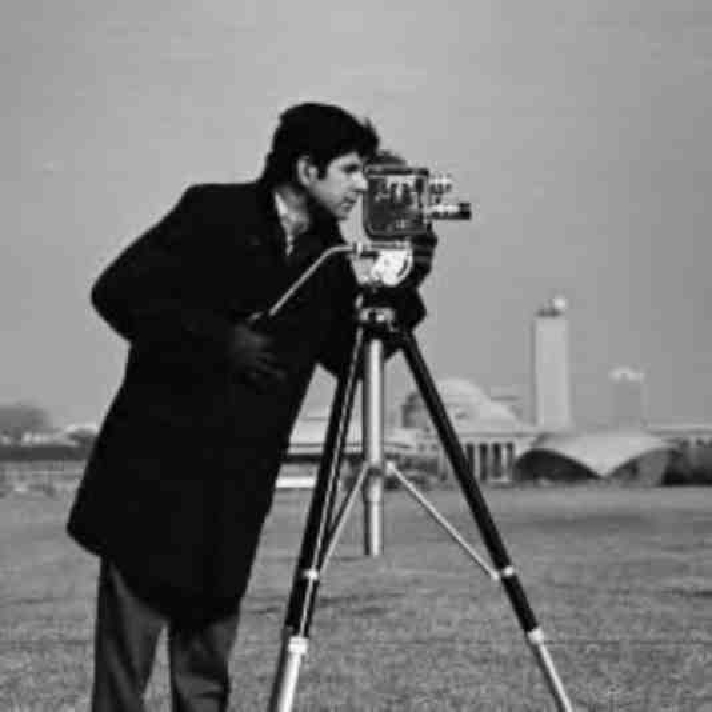
\includegraphics[width=8cm, height=8cm]{man-unmodified.jpg}
	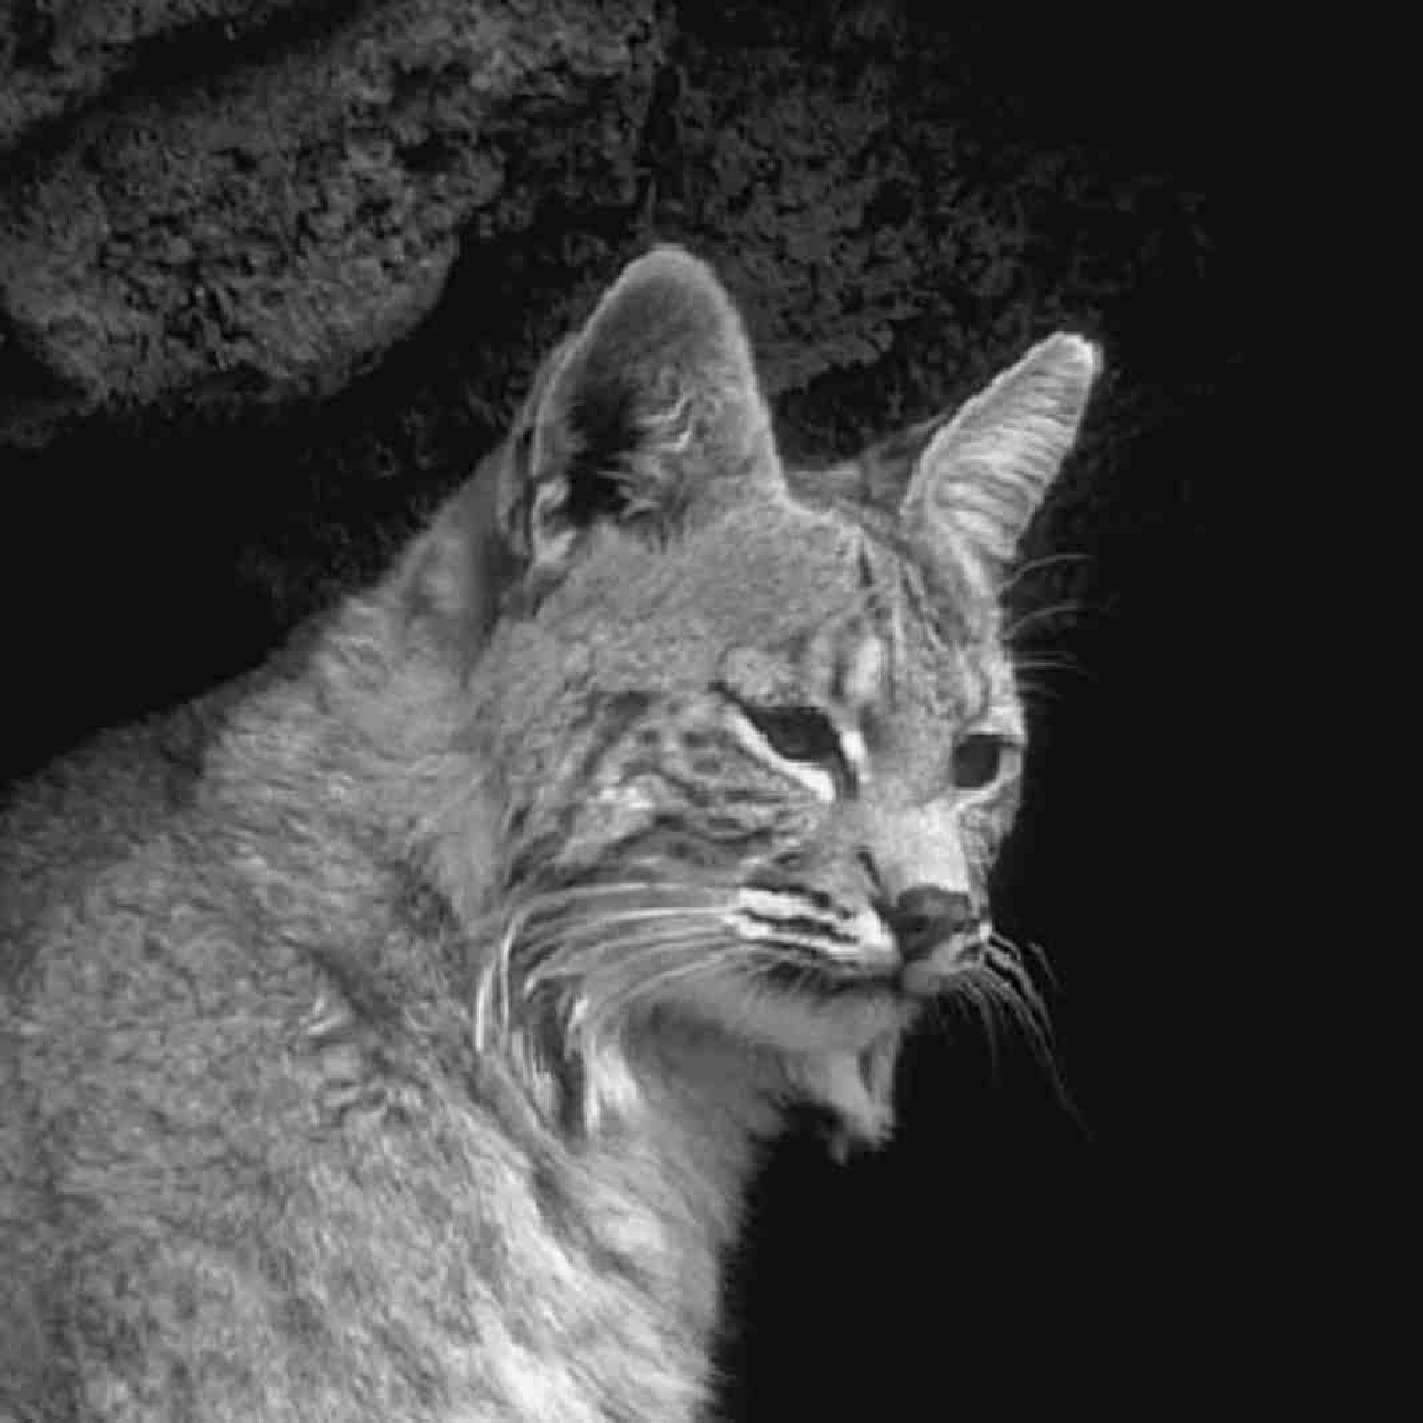
\includegraphics[width=8cm, height=8cm]{cat-unmodified.jpg}
\end{figure}
\begin{figure}
	\caption{Po uruchomieniem algorytmu (od lewej): obraz 1 (2133x2133, 300dpi), obraz 2 (2133x2133, 300dpi)}
	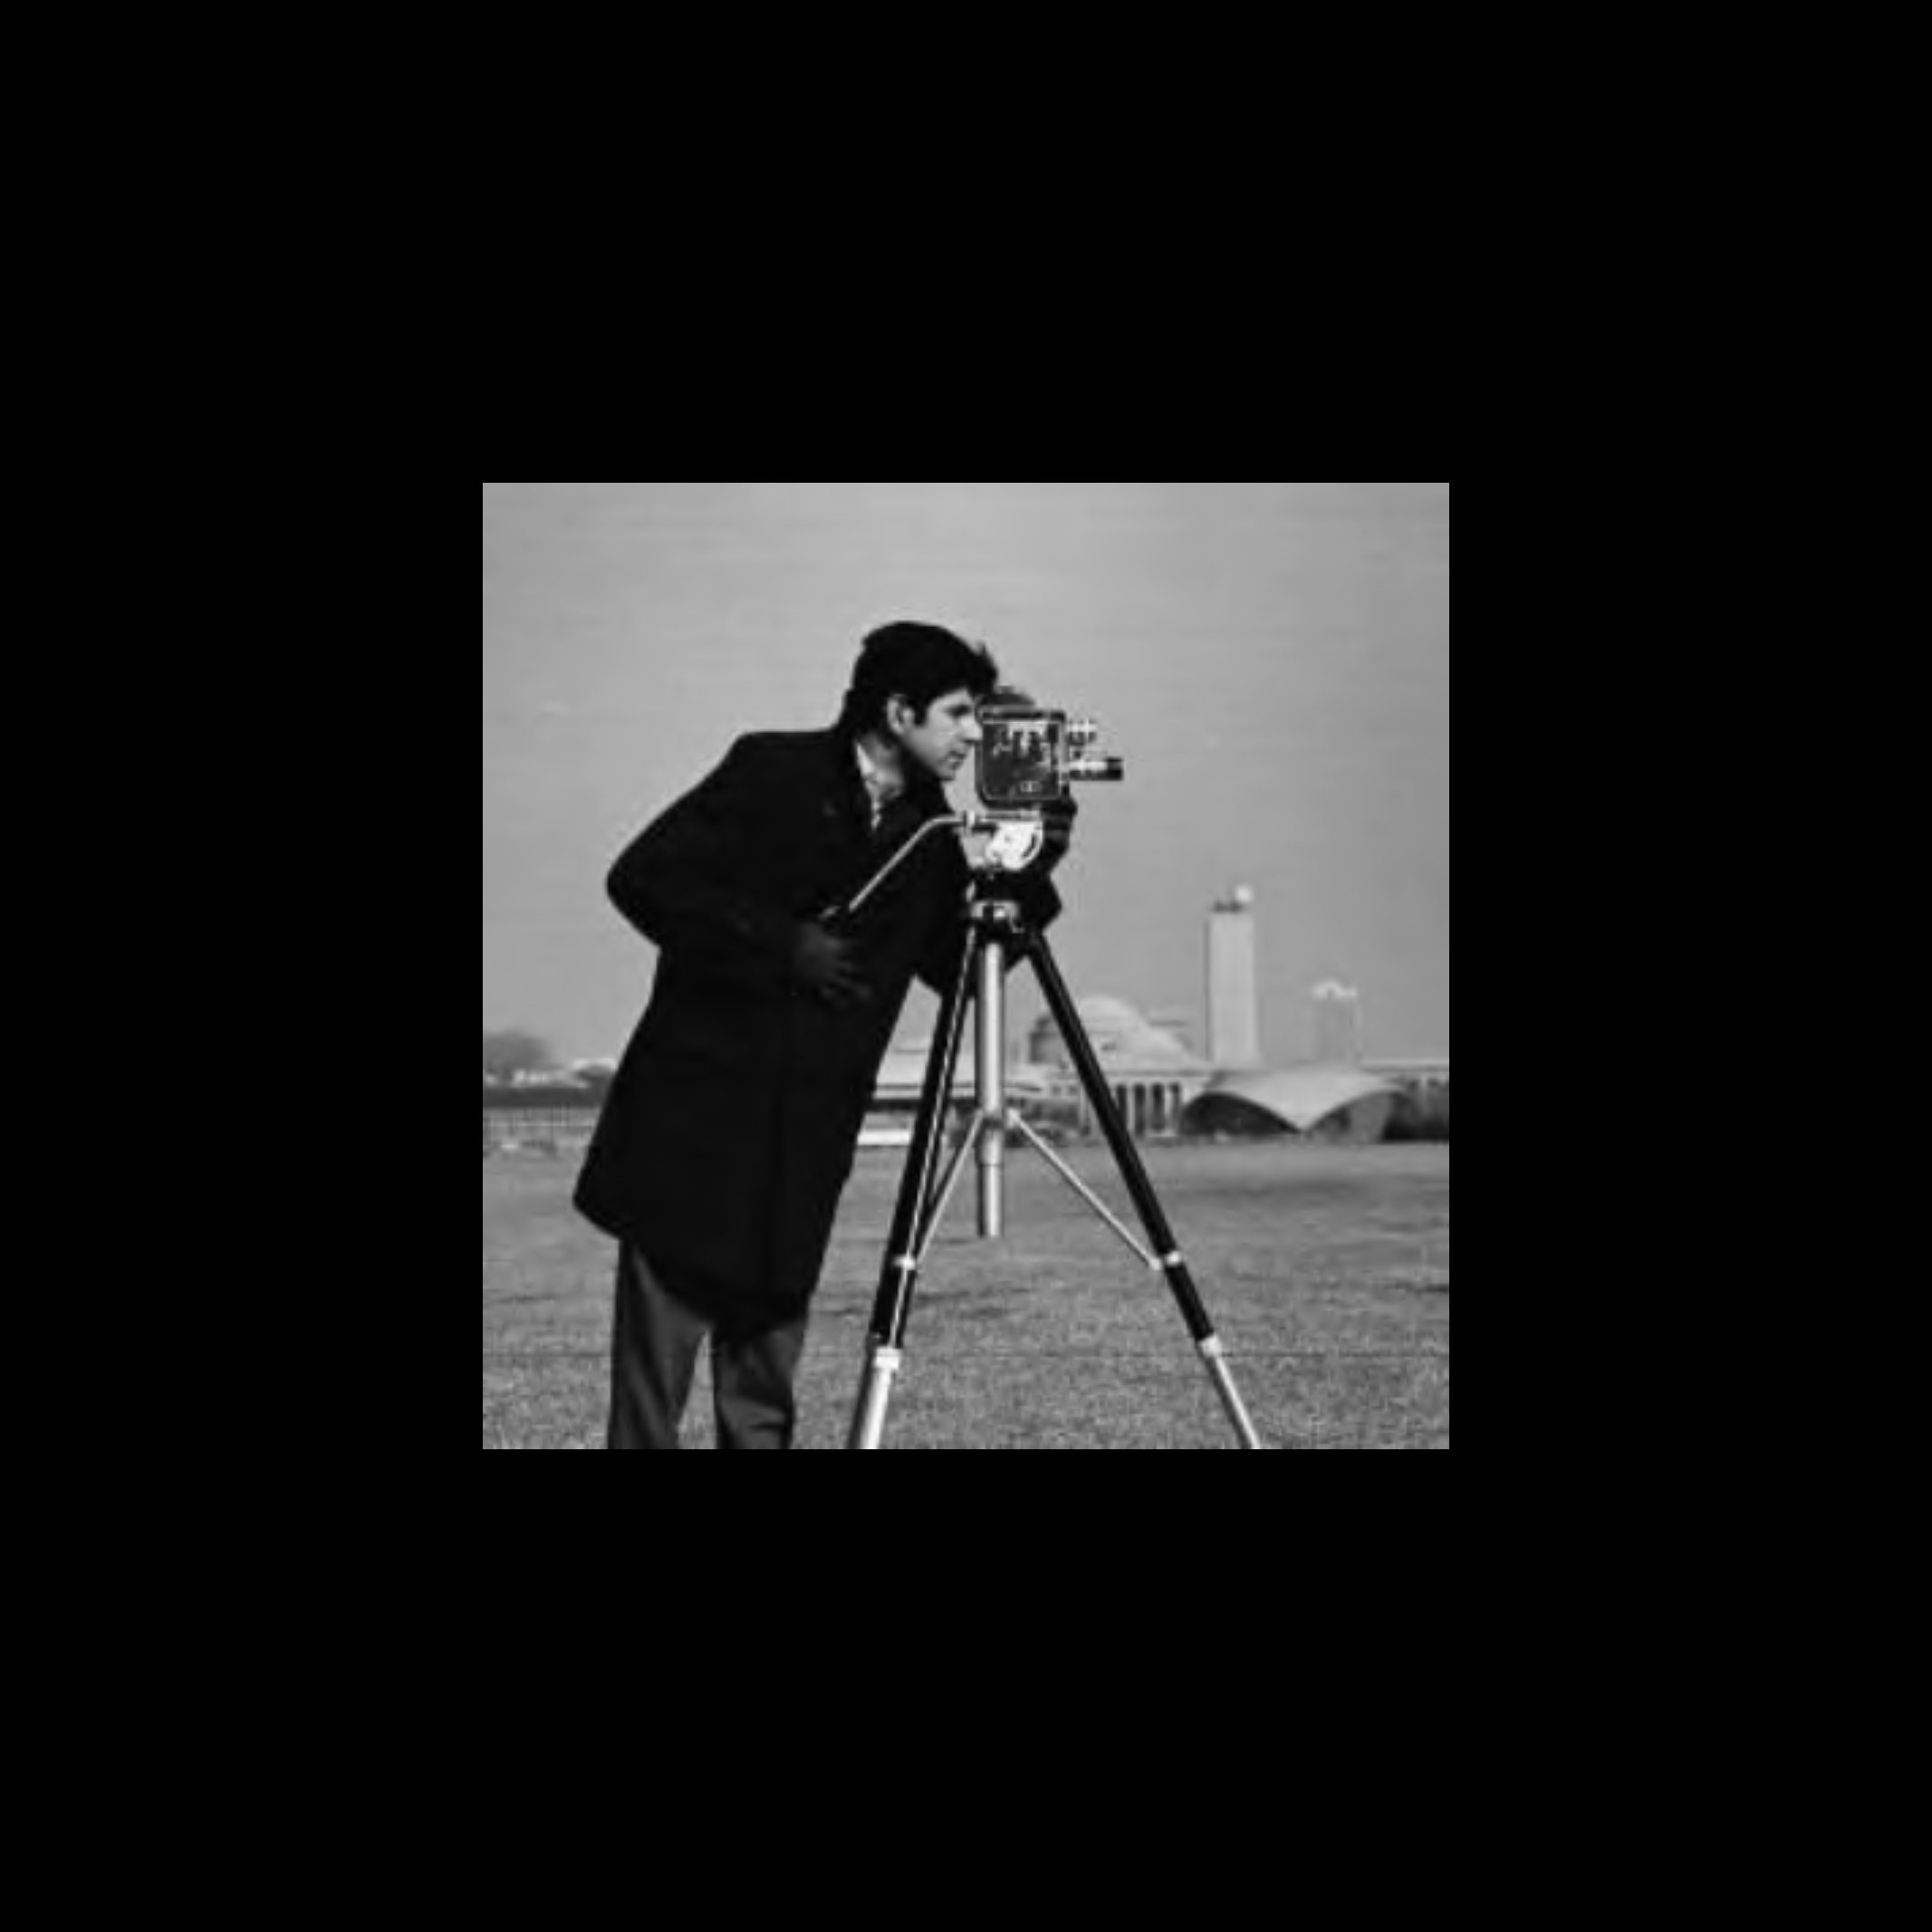
\includegraphics[width=8cm, height=8cm]{man-modified.png}
	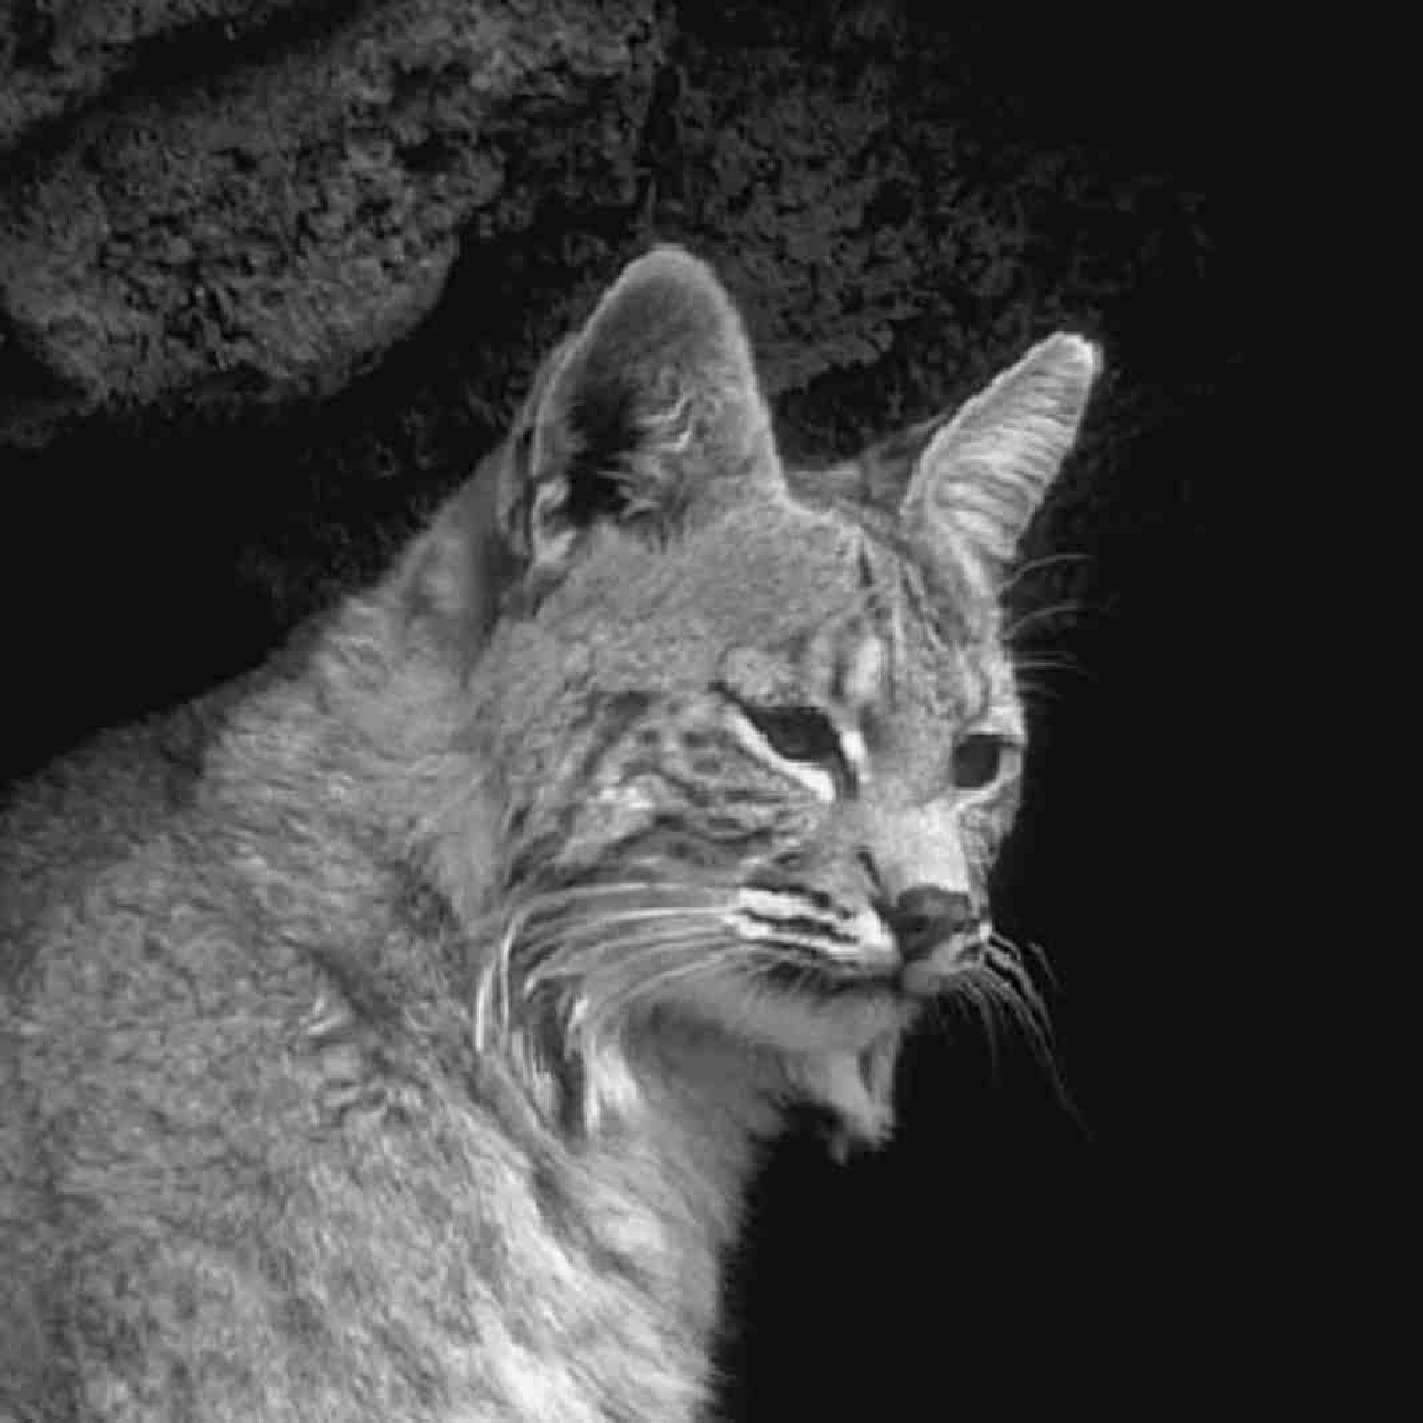
\includegraphics[width=8cm, height=8cm]{cat-unmodified.jpg}
\end{figure}
\subsection*{Kod źródłowy algorytmu}
\begin{python}
def geometricGray(self):
	print('geometric gray unificaiton start')
	width, height = self.firstDecoder.width, self.firstDecoder.height
	if width < self.maxWidth or height < self.maxHeight:
		# Create black background
		firstResult = numpy.zeros((self.maxHeight, self.maxWidth), numpy.uint8)
		# Copy smaller image to bigger
		startWidthIndex = int(round((self.maxWidth - width) / 2))
		startHeightIndex = int(round((self.maxHeight - height) / 2))
		pixelsBuffer = self.firstDecoder.getPixels()
		for h in range (0, height):
		for w in range (0, width):
		firstResult[h + startHeightIndex, w + startWidthIndex] = pixelsBuffer[h, w]
		img = Image.fromarray(firstResult, mode='L')
		img.save('Resources/ggUnification_1.png')
		print('first image done')
	
	width, height = self.secondDecoder.width, self.secondDecoder.height
	if width < self.maxWidth or height < self.maxHeight:
		# Create black background
		secondResult = numpy.zeros((self.maxHeight, self.maxWidth), numpy.uint8)
		# Copy smaller image to bigger
		startWidthIndex = int(round((self.maxWidth - width) / 2))
		startHeightIndex = int(round((self.maxHeight - height) / 2))
		pixelsBuffer = self.secondDecoder.getPixels()
		for h in range (0, height):
		for w in range (0, width):
		secondResult[h + startHeightIndex, w + startWidthIndex] = pixelsBuffer[h, w]
		img = Image.fromarray(secondResult, mode='L')
		img.save('Resources/ggUnification_2.png')
		print('second image done')
	print('geometric gray unification done')
\end{python}
\section{Ujednolicenie obrazów szarych rozdzielczościowe}
\subsection*{Algorytm}
\subsubsection*{Opis}
Po użyciu ujednolicenia geometrycznego można użyć ujednolicenia rozdzielczościowego, które przeskaluje obraz z mniejszej postaci do większej dzięki czemu nie zostanie nam czarna ramka wokół obrazu. Wynikiem będzie większy obraz niż początkowo bez czarnego obwodu wokół. 
Mniejszy obraz można przeskalować do większych wymiarów przenosząc wszystkie piksele z uwzględnieniem luk pomiędzy nimi i następnie użycia interpolacji do zamazania tych luk. 
Interpolacja działa na zasadzie pobierania wartości z okolicznych pikseli i wyciągania z nich średniej, która posłuży jako baza koloru dla nowego piksela. 
\subsubsection*{Kroki}
\begin{enumerate}
	\item Ustalenie nowych wymiarów obrazu
	\item Obliczenie odległości pomiędzy pikselami (\textit{scaleFactoryH, scaleFactoryW})
	\item Naniesienie pikseli z mniejszego obrazu na większy z uwzględnieniem luk
	\item Interpolacja
\end{enumerate}
\begin{figure}
	\caption{Skutki braku interpolacji}
	\begin{center}
		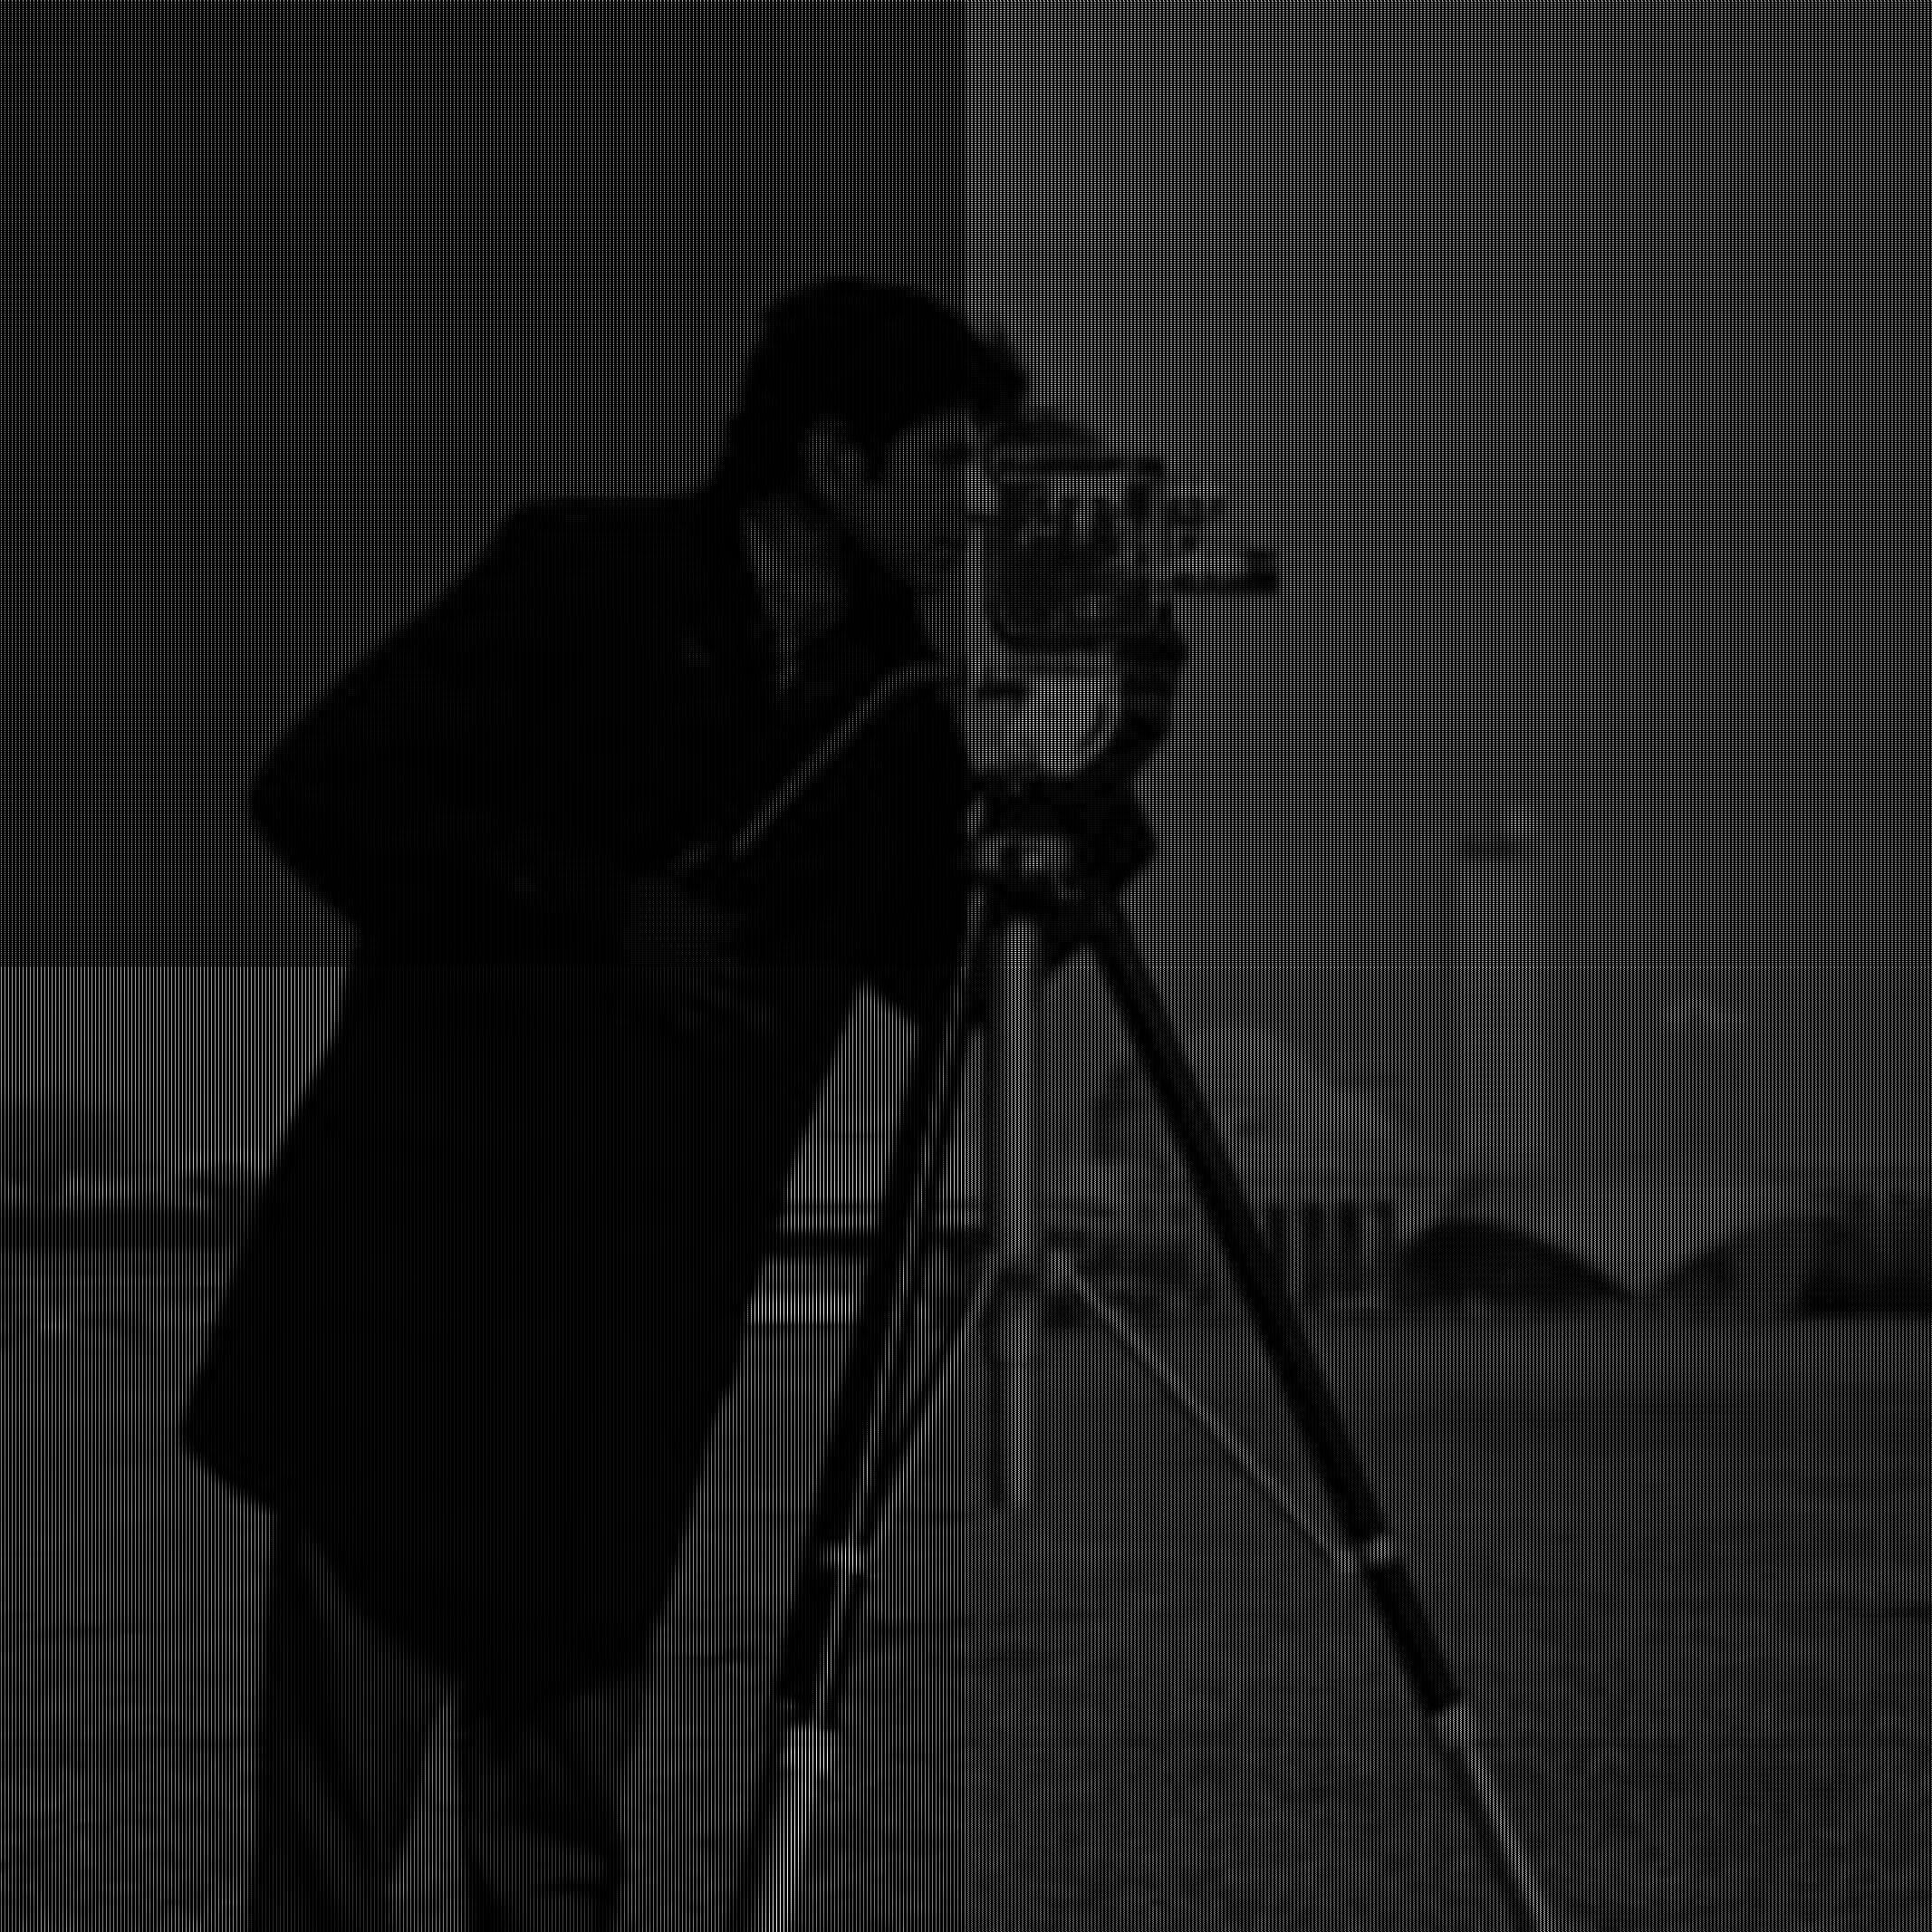
\includegraphics[width=8cm, height=8cm]{man-without-interpolation.png}
	\end{center}
\end{figure}
\begin{figure}
	\caption{Przed uruchomieniem algorytmu (od lewej): obraz 1 (2133x2133, 300dpi), obraz 2 (2133x2133, 300dpi)}
	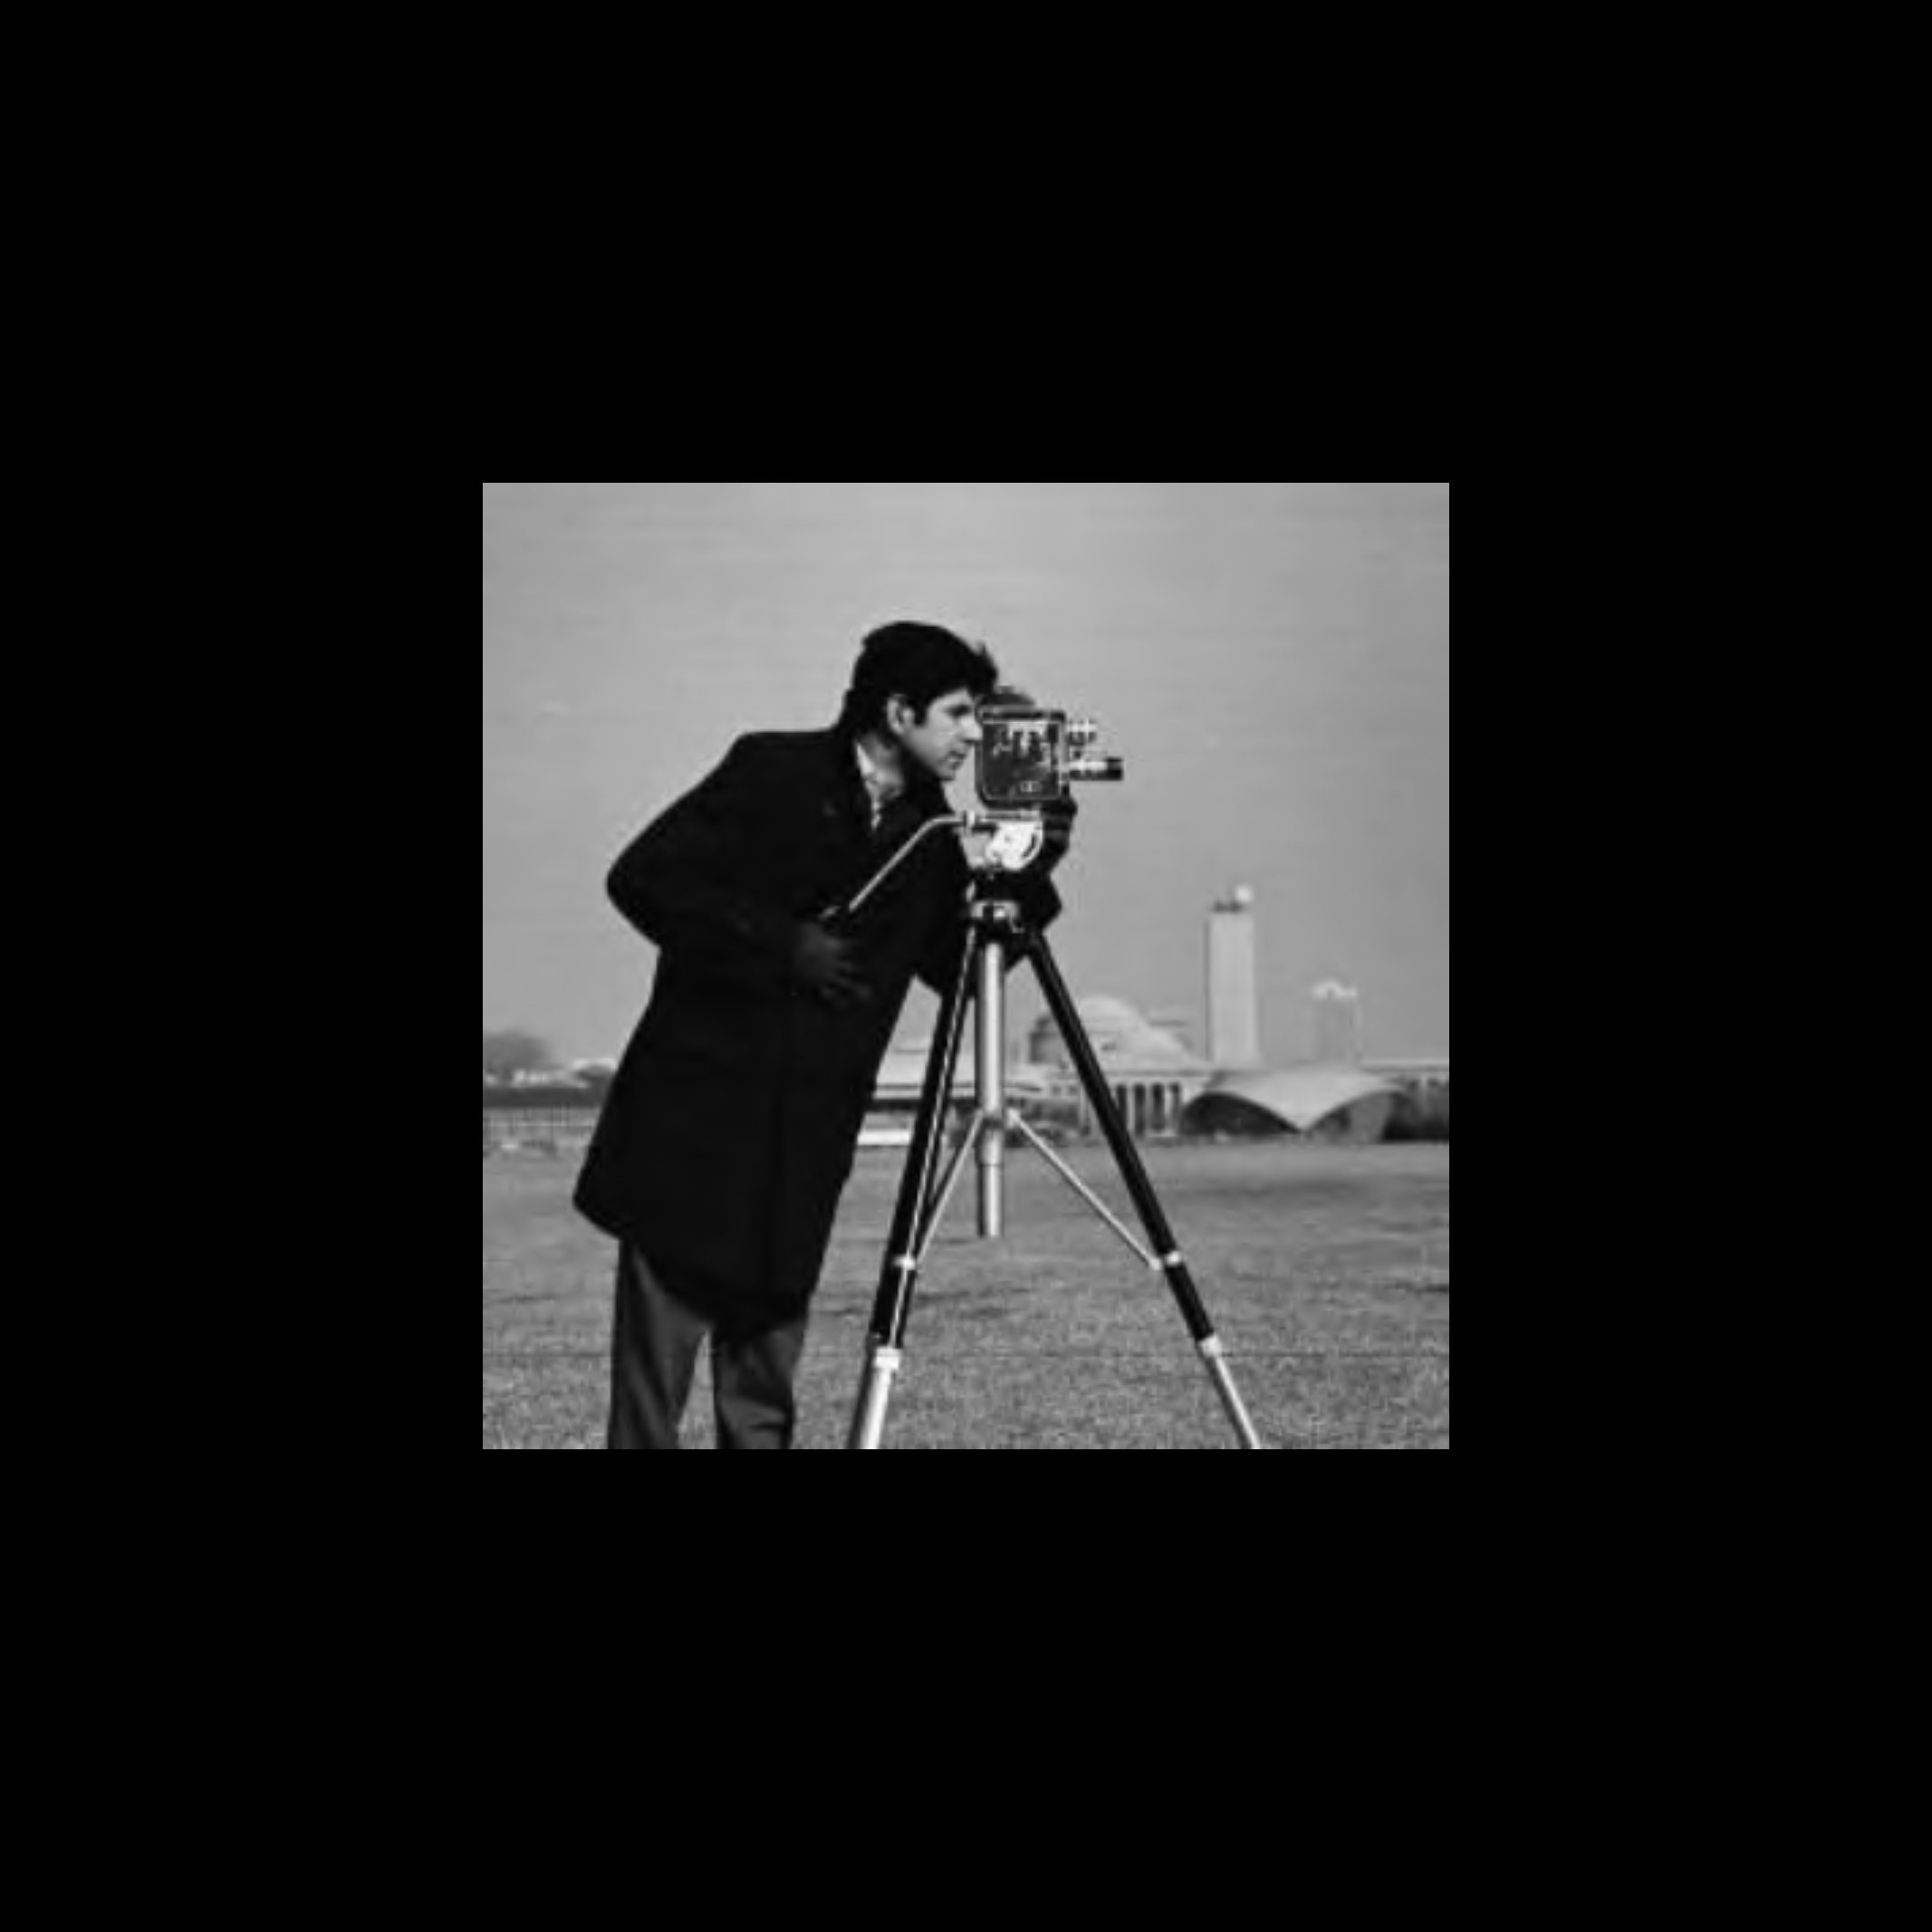
\includegraphics[width=8cm, height=8cm]{man-modified.png}
	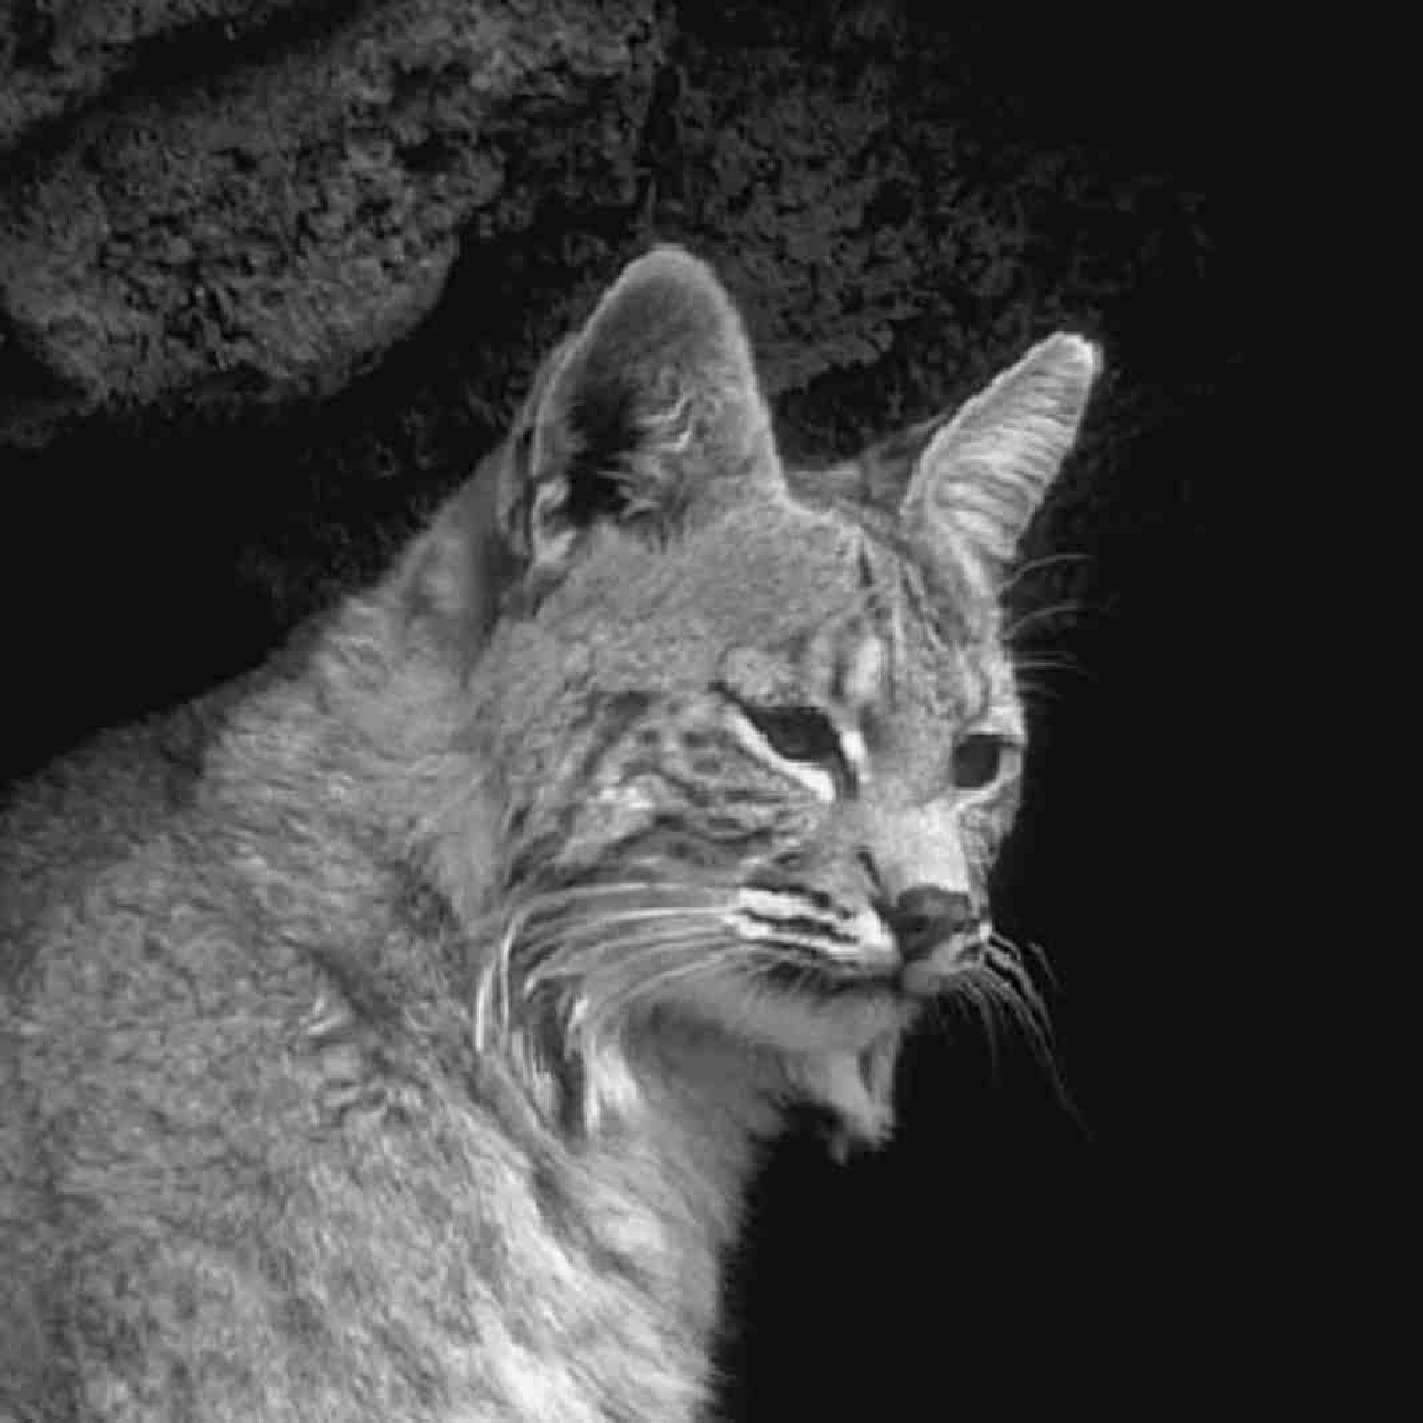
\includegraphics[width=8cm, height=8cm]{cat-unmodified.jpg}
\end{figure}
\begin{figure}
	\caption{Po uruchomieniem algorytmu (od lewej): obraz 1 (2133x2133, 300dpi), obraz 2 (2133x2133, 300dpi)}
	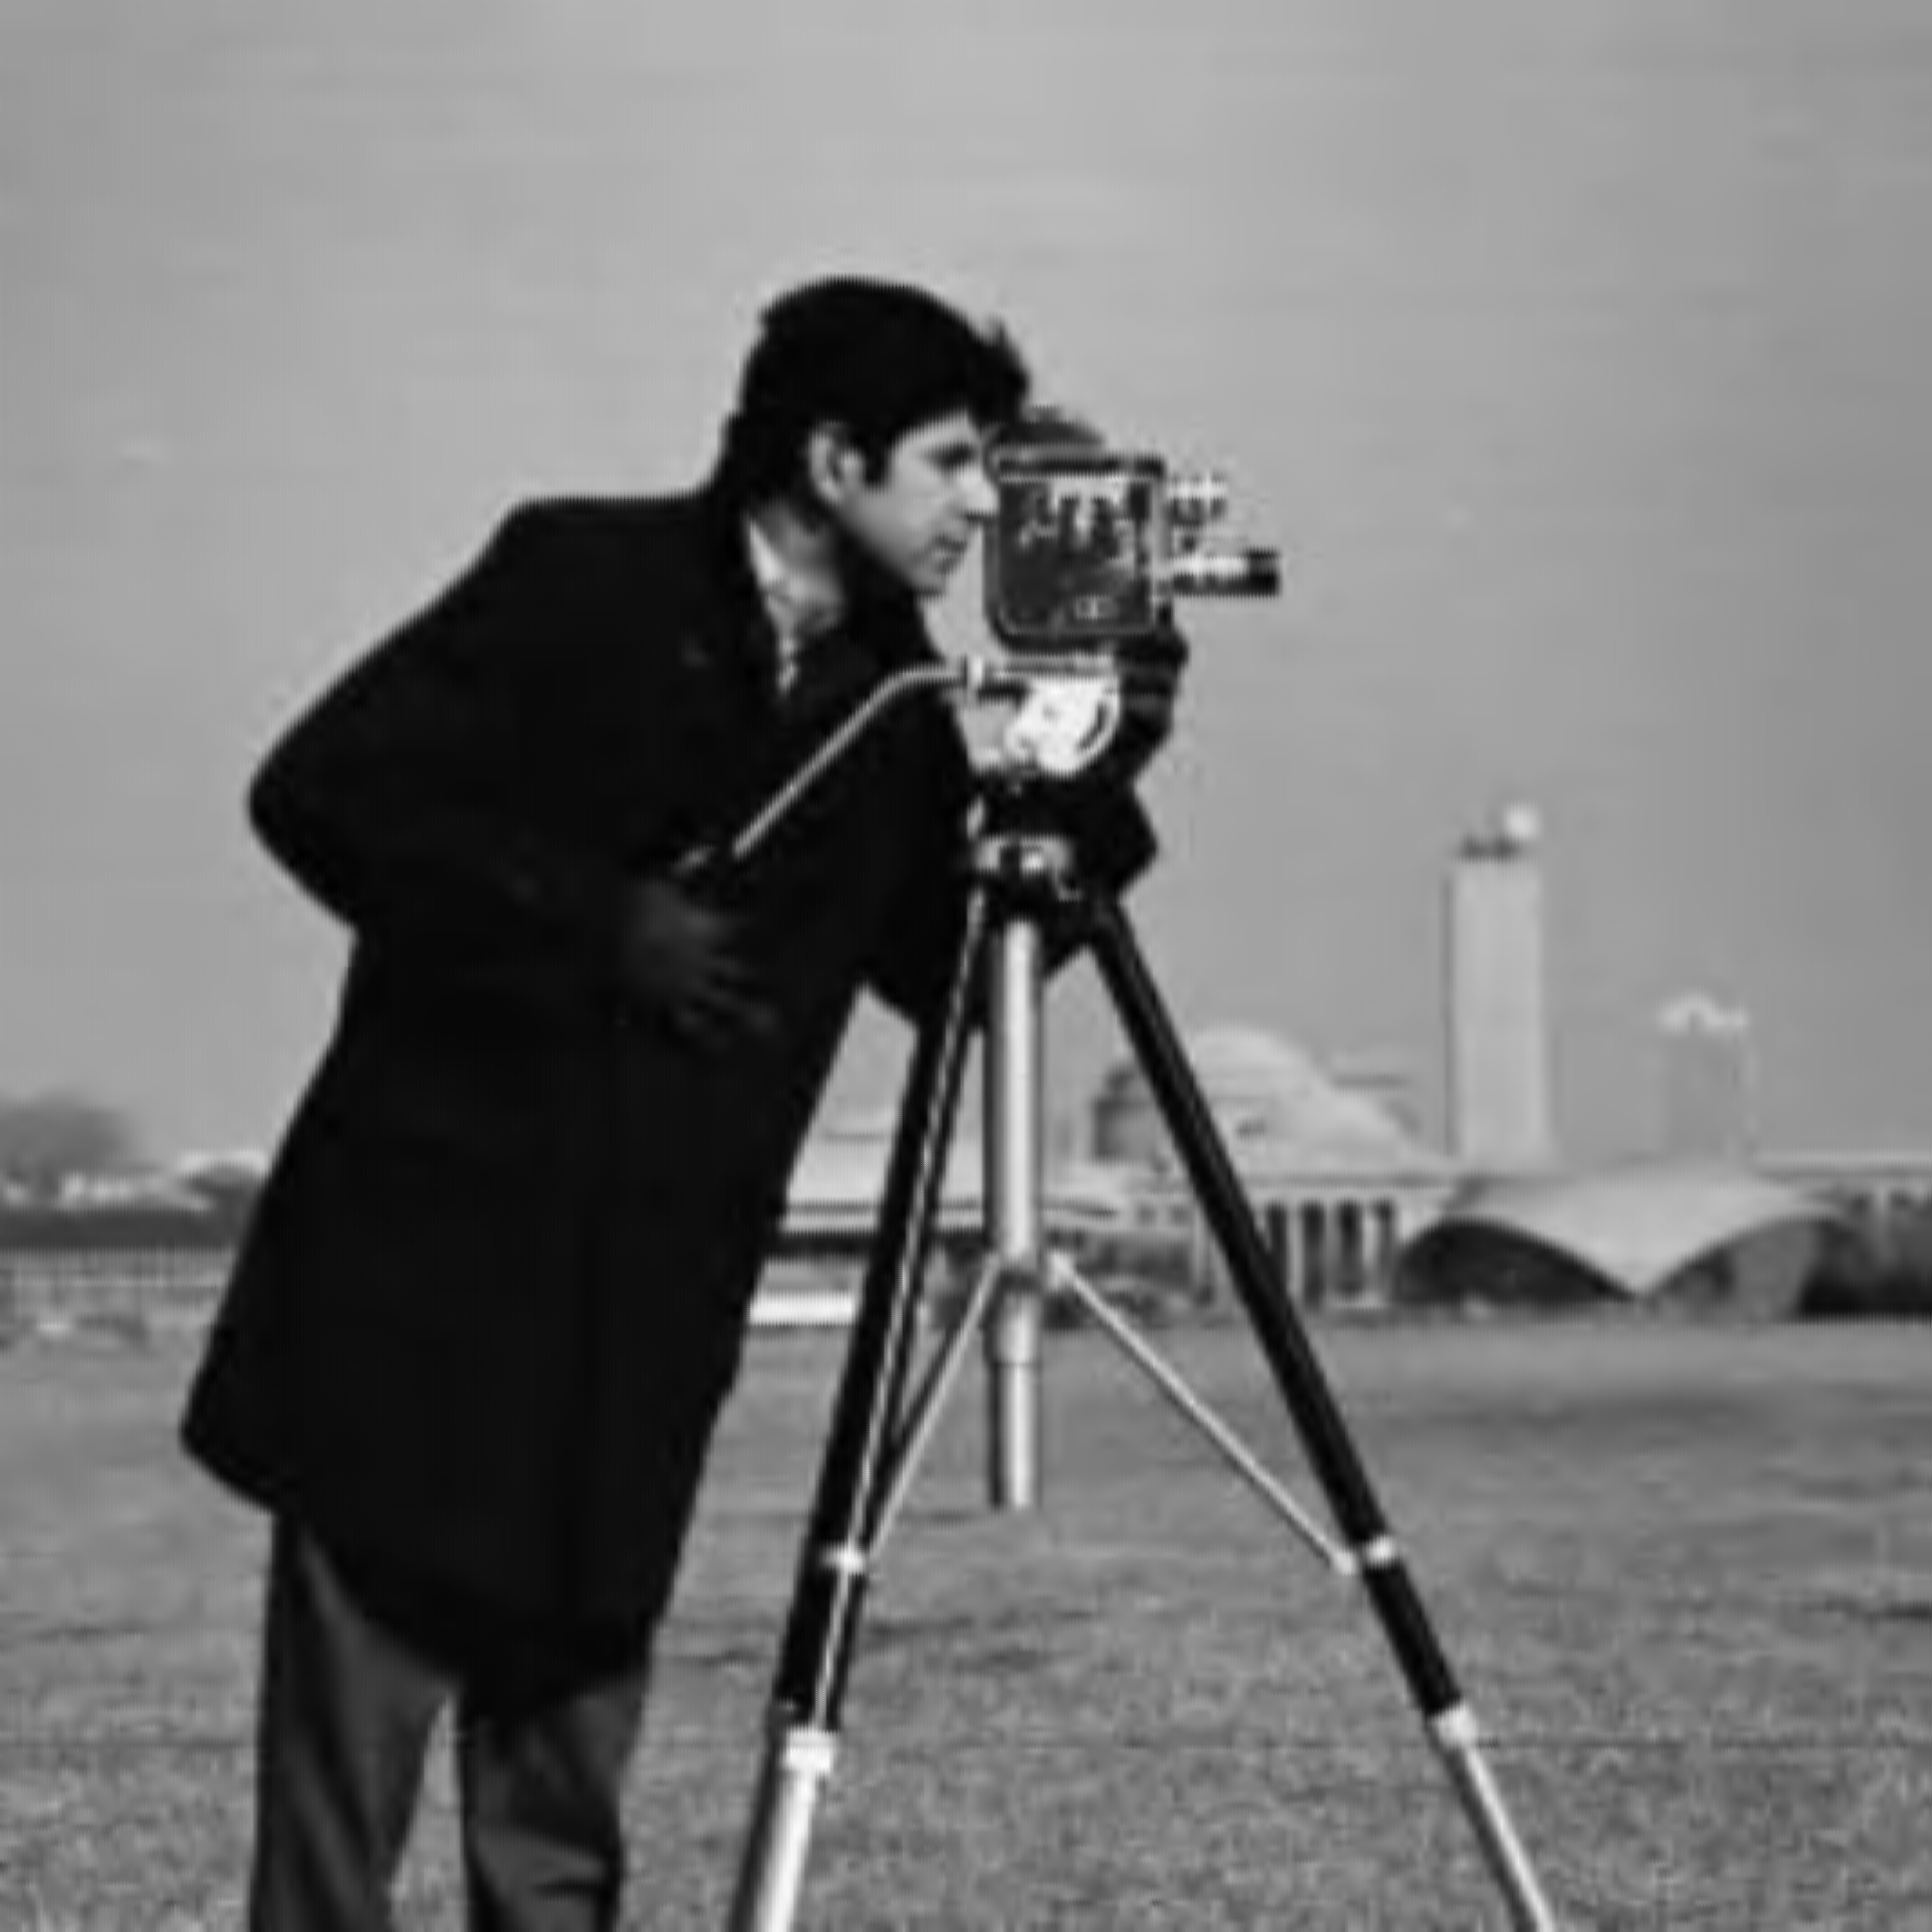
\includegraphics[width=8cm, height=8cm]{man-rastar-unification.png}
	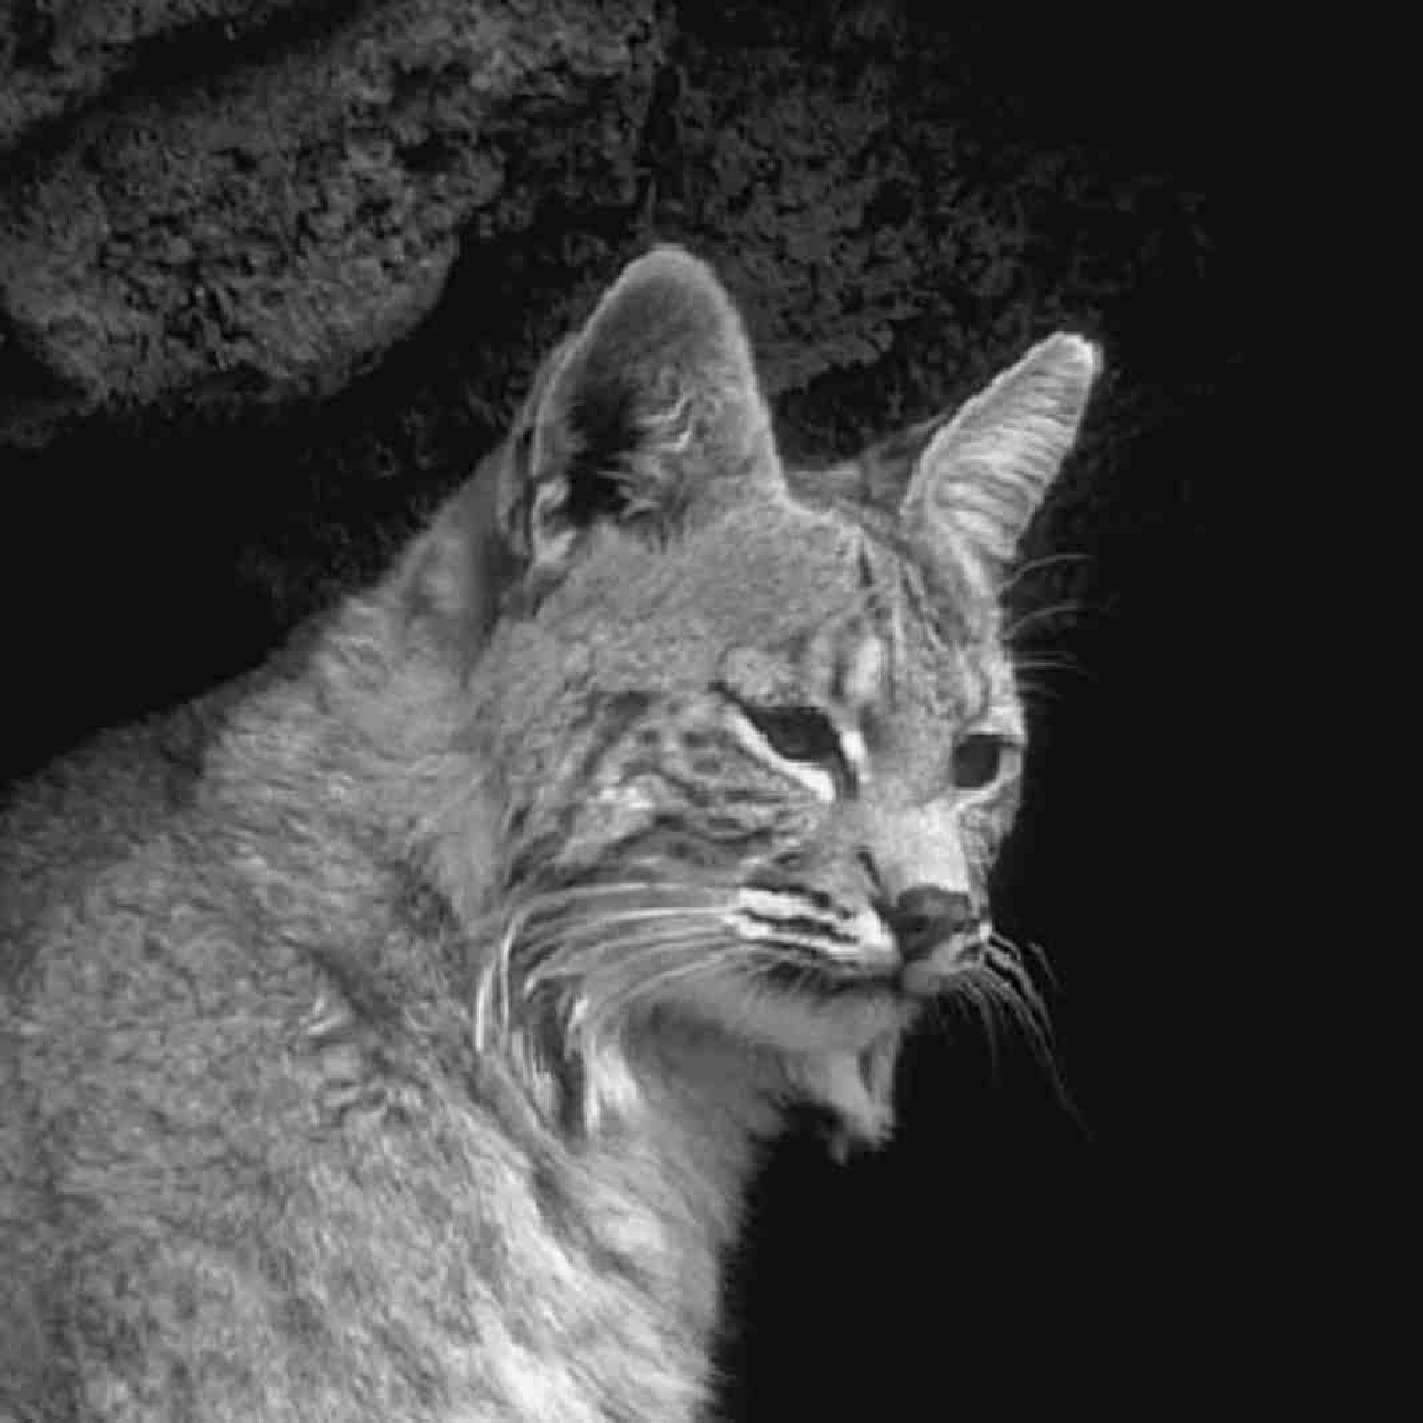
\includegraphics[width=8cm, height=8cm]{cat-unmodified.jpg}
\end{figure}
\subsection*{Kod źródłowy algorytmu}
\begin{python}
def rasterGray(self):
	print('raster gray unification start')
	self._scaleUpGray(self.firstDecoder, 'Resources/rgUnification_1.png')
	print('first image done')
	self._scaleUpGray(self.secondDecoder, 'Resources/rgUnification_2.png')
	print('second image done')
	print('raster gray unification done')

def _scaleUpGray(self, decoder, outputPath):
	width, height = decoder.width, decoder.height
	scaleFactoryW = float(self.maxWidth) / width
	scaleFactoryH = float(self.maxHeight) / height
	if width < self.maxWidth or height < self.maxHeight:
		pixelsBuffer = decoder.getPixels()
		result = numpy.zeros((self.maxHeight, self.maxWidth), numpy.uint8)
		# Fill values
		for h in range(height):
			for w in range(width):
				if w%2 == 0:
					result[int(scaleFactoryH * h), int(round(scaleFactoryW * w)) + 1] = pixelsBuffer[h, w]
				if w%2 == 1:
					result[int(round(scaleFactoryH * h)) + 1, int(scaleFactoryW * w)] = pixelsBuffer[h, w]
		# Interpolate
		self._interpolateGray(result)
		img = Image.fromarray(result, mode='L')
		img.save(outputPath)

def _interpolateGray(self, result):
	for h in range(self.maxHeight):
		for w in range(self.maxWidth):
			value = 0
			count = 0
			if result[h, w] == 0:
				for hOff in range(-1, 2):
					for wOff in range(-1, 2):
						hSafe = h if ((h + hOff) > (self.maxHeight - 2)) | ((h + hOff) < 0) else (h + hOff)
						wSafe = w if ((w + wOff) > (self.maxWidth - 2)) | ((w + wOff) < 0) else (w + wOff)
						if result[hSafe, wSafe] != 0:
							value += result[hSafe, wSafe]
							count += 1
				result[h, w] = value / count
\end{python}
\section{Ujednolicenie obrazów RGB geometryczne}
\subsection*{Algorytm}
\subsubsection*{Opis}
Algorytm geometrycznego ujednolicenia obrazów ma za zadanie sprowadzić oba obrazy do tej samej liczby pikseli w każdym wierszu i każdej kolumnie. 
Różnica pomiędzy tym przypadkiem a szarym sprawia, że ważne jest użycie odpowiednich struktur danych w taki sposób aby każdy z kanałów RGB był w stanie się pomieścić. Niewątpliwie ważne jest struktura danych uwzględniała kolejność w jakim kolory są przechowywane, inaczej może dojść do sytuacji w której nie dostaniemy oczekiwanego rezultatu. 
\subsubsection*{Kroki}
\begin{enumerate}
	\item Porównaj szerokości i wysokości obu obrazów i wybierz największe. 
	\item Jeśli pierwszy lub drugi obraz mają szerokość lub wysokość mniejszą od największej dostępnej to:
	\begin{enumerate}
		\item Utwórz czarne tło
		\item Przenieś z wyśrodkowaniem piksle na czarne tło z uwzględnieniem każdego z kanałów RGB
	\end{enumerate}
	\item Jeśli żaden z warunków jest niespełniony to nie rób nic
\end{enumerate}
\begin{figure}
	\caption{Przed uruchomieniem algorytmu (od lewej): obraz 1 (512x512, 300dpi), obraz 2 (1024x1024, 300dpi)}
	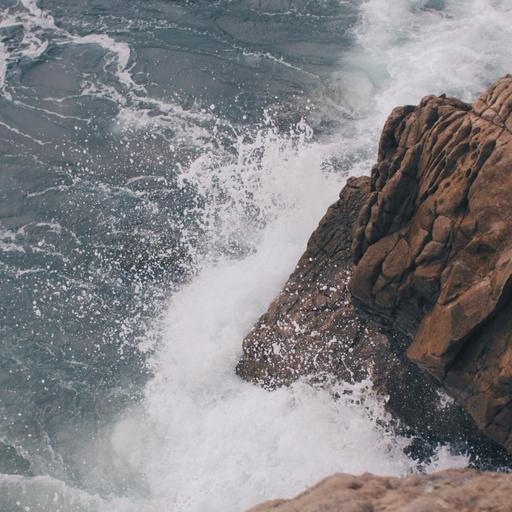
\includegraphics[width=8cm, height=8cm]{sea-unmodified.jpg}
	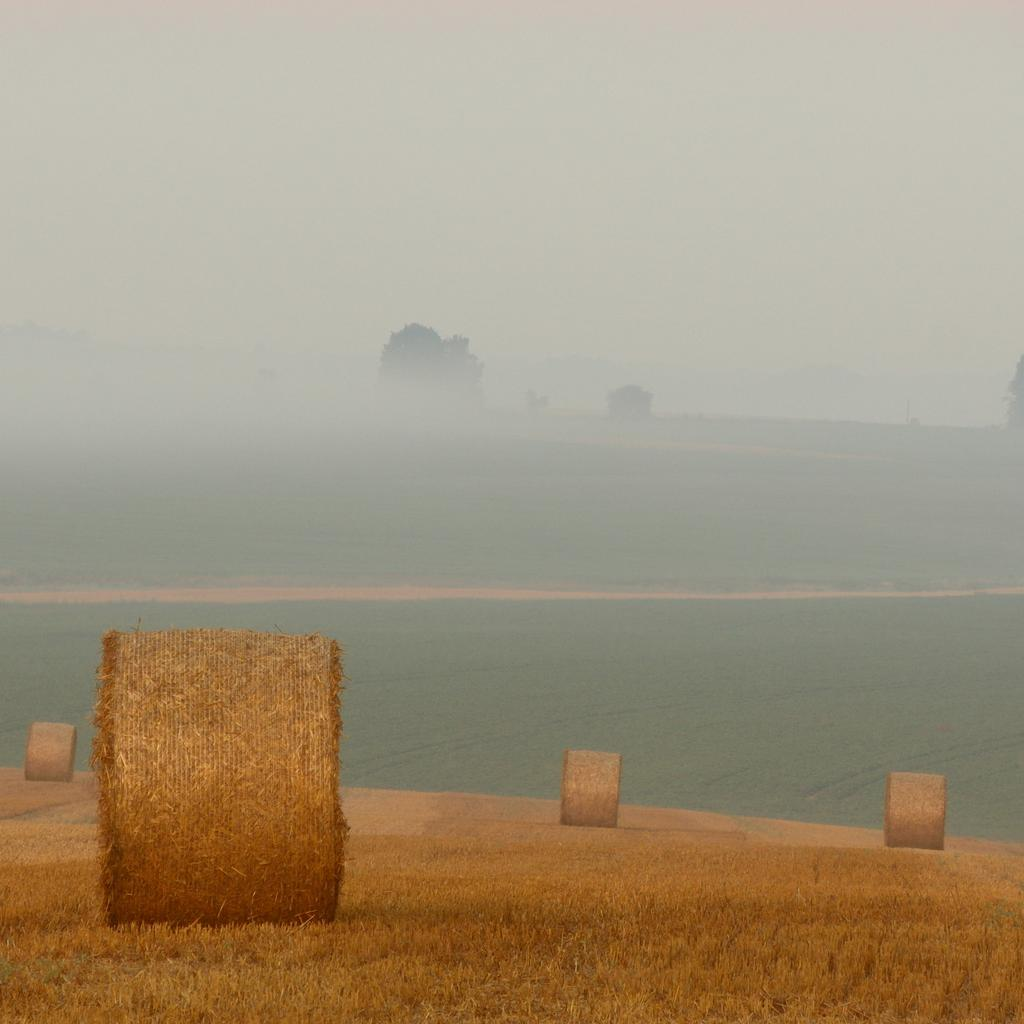
\includegraphics[width=8cm, height=8cm]{field-unmodified.jpg}
\end{figure}
\begin{figure}
	\caption{Po uruchomieniem algorytmu (od lewej): obraz 1 (1024x1024, 300dpi), obraz 2 (1024x1024, 300dpi)}
	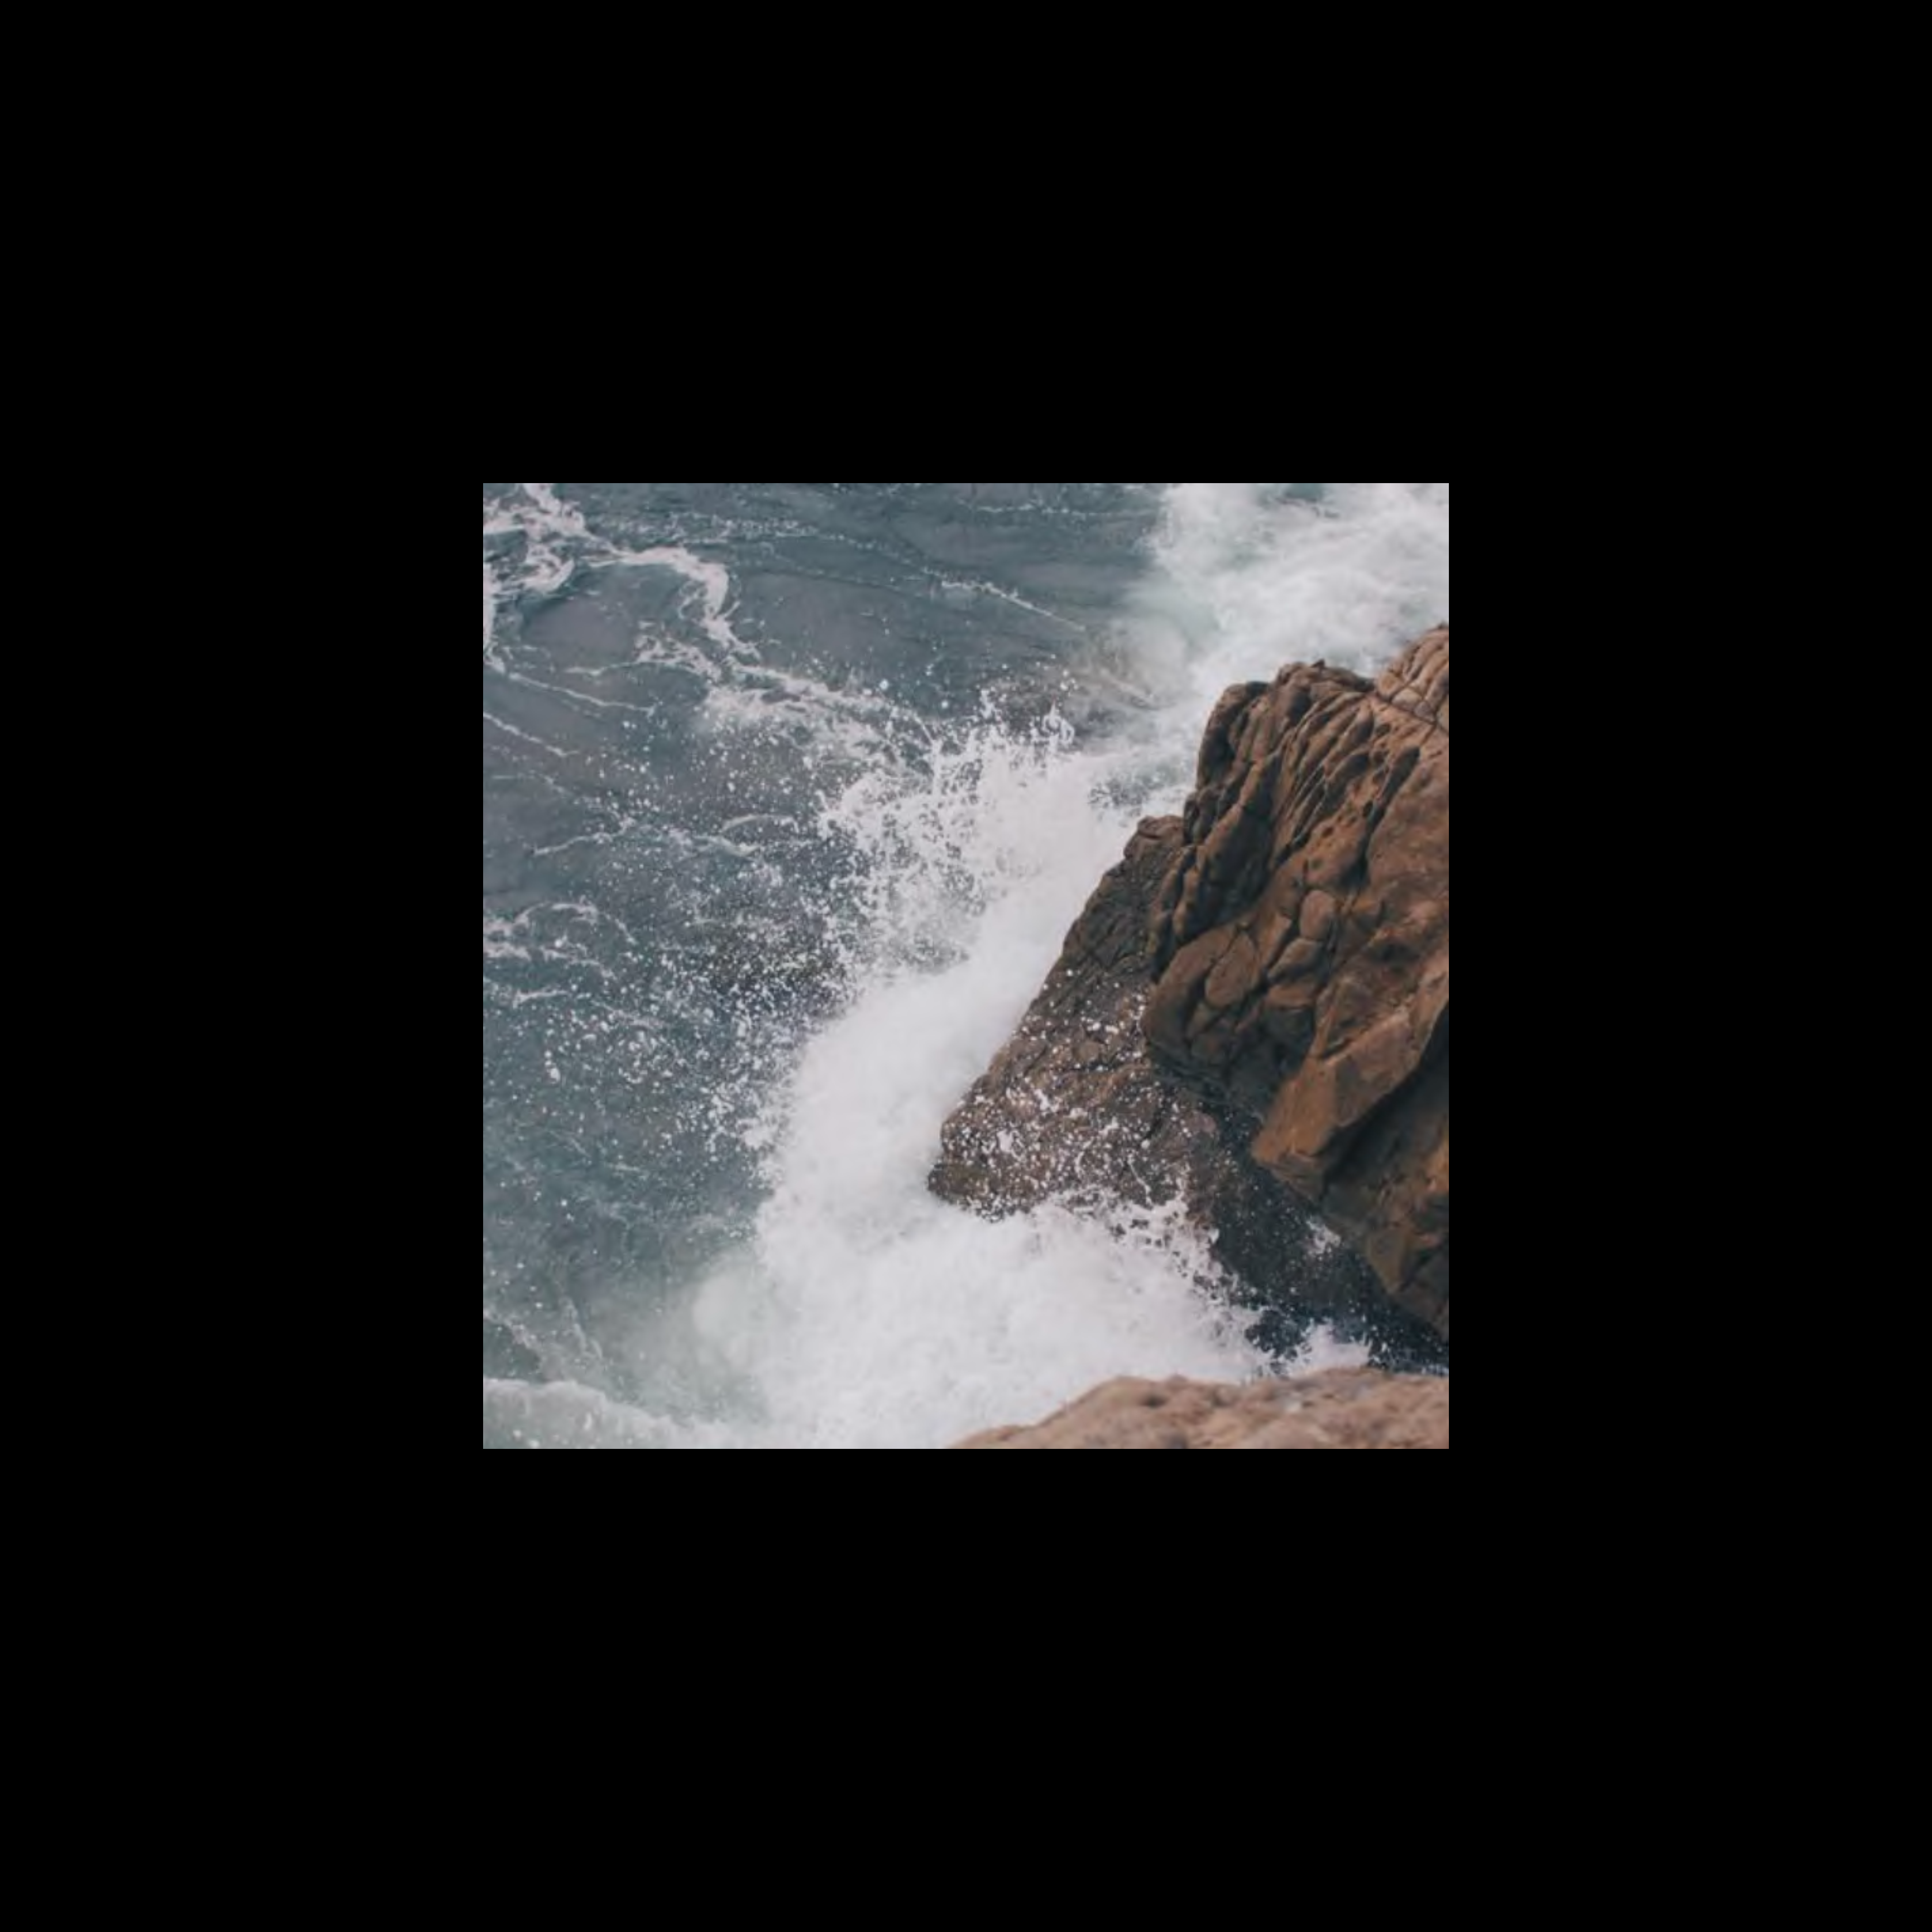
\includegraphics[width=8cm, height=8cm]{sea-geo-modified.png}
	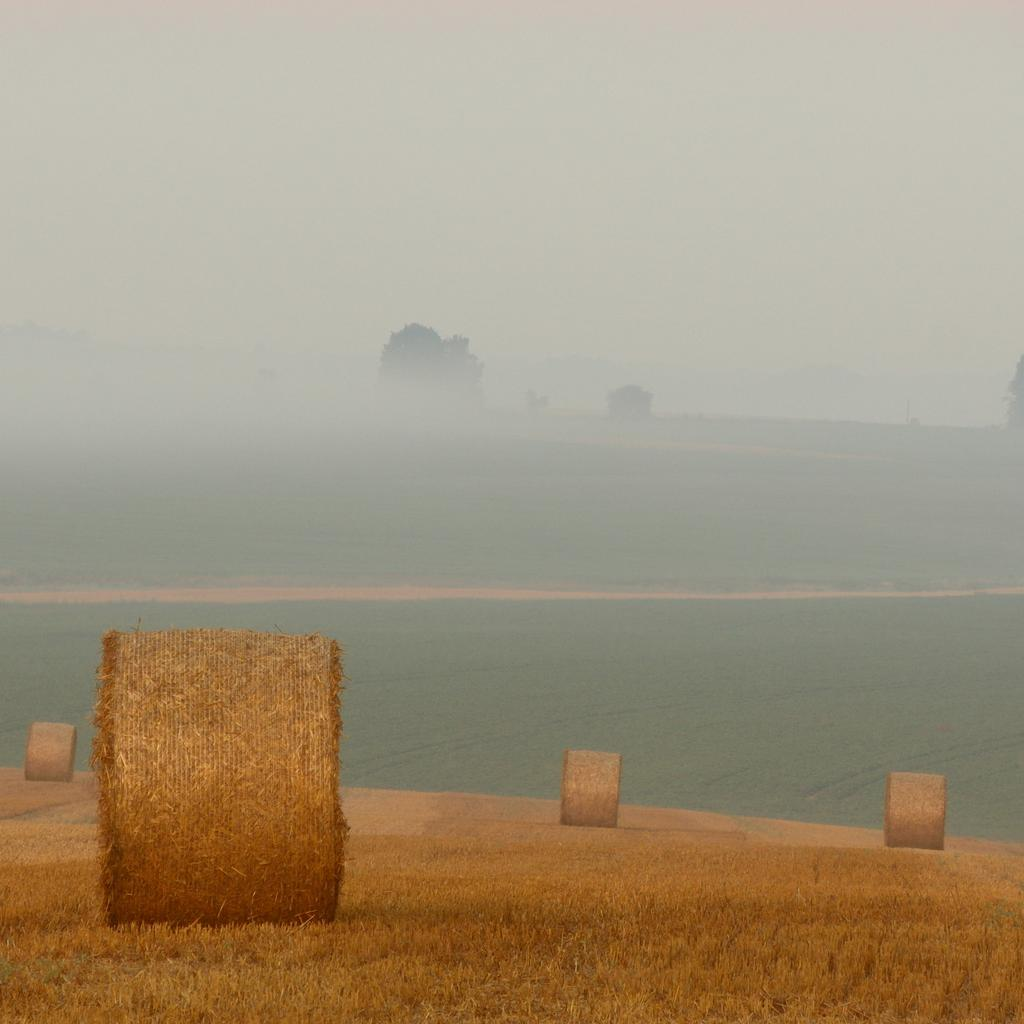
\includegraphics[width=8cm, height=8cm]{field-unmodified.jpg}
\end{figure}
\begin{figure}
	\caption{Przed uruchomieniem algorytmu (od lewej): obraz 3 (126x126, 300dpi), obraz 4 (256x256, 300dpi)}
	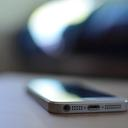
\includegraphics[width=8cm, height=8cm]{phone-unmodified.jpg}
	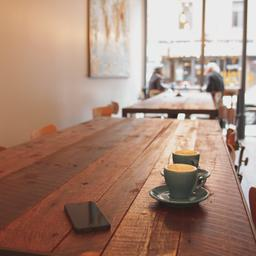
\includegraphics[width=8cm, height=8cm]{coffee-unmodified.jpg}
\end{figure}
\begin{figure}
	\caption{Po uruchomieniem algorytmu (od lewej): obraz 3 (126x126, 300dpi), obraz 4 (256x256, 300dpi)}
	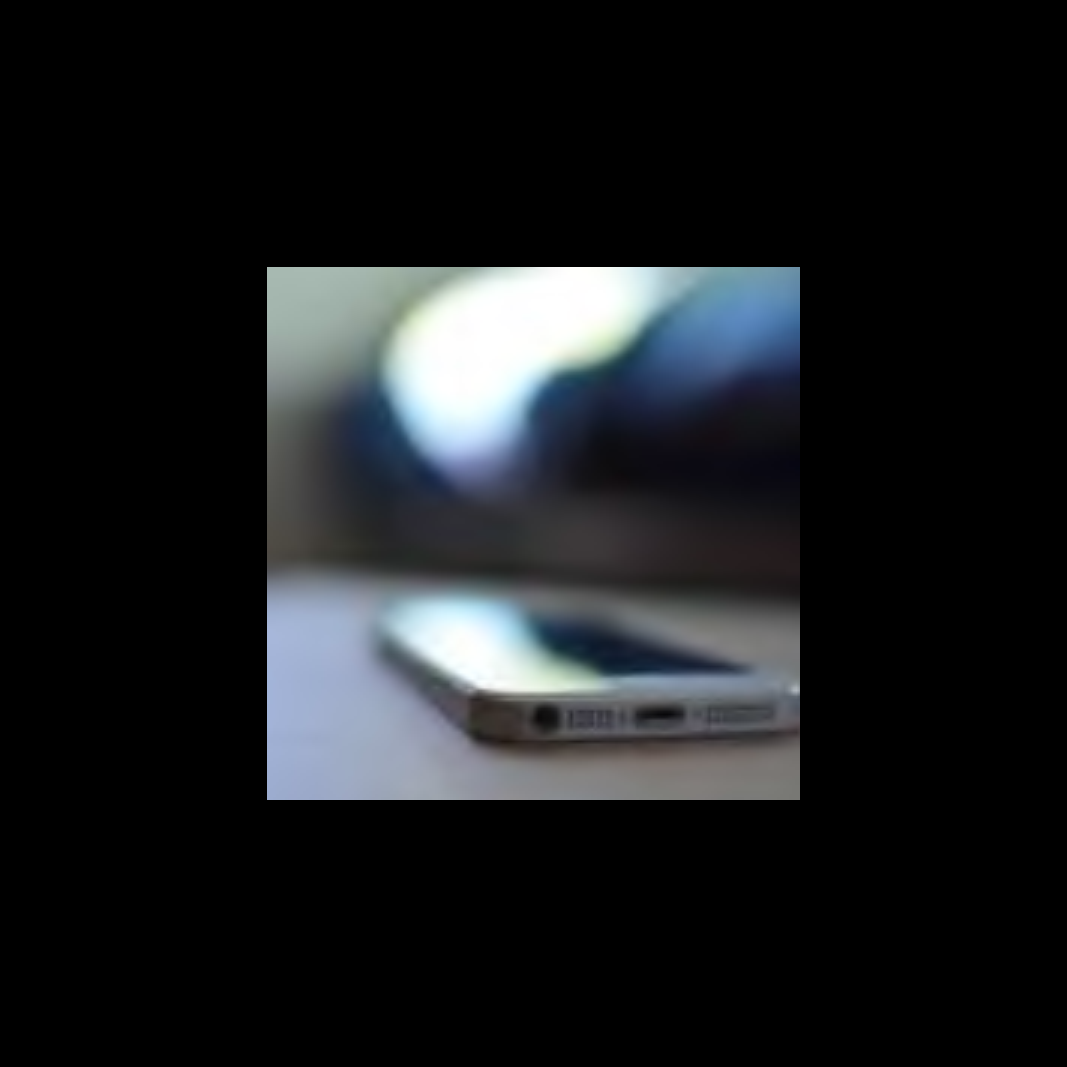
\includegraphics[width=8cm, height=8cm]{phone-geo-modified.png}
	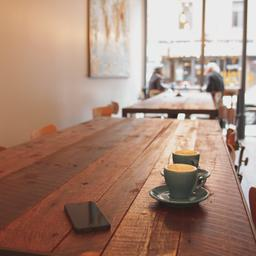
\includegraphics[width=8cm, height=8cm]{coffee-unmodified.jpg}
\end{figure}
\newpage
\subsection*{Kod źródłowy algorytmu}
\begin{python}
def geometricColor(self):
	print('geometric color unificaiton start')
	self.firstDecoder.setColor()
	width, height = self.firstDecoder.width, self.firstDecoder.height
	if width < self.maxWidth or height < self.maxHeight:
		result = self._paintInMiddleColor(self.firstDecoder)
		img = Image.fromarray(result, 'RGB')
		img.save('Resources/gcUnification_1.png')
		print('first image done')
	
	self.secondDecoder.setColor()
	width, height = self.secondDecoder.width, self.secondDecoder.height
	if width < self.maxWidth or height < self.maxHeight:
		result = self._paintInMiddleColor(self.secondDecoder)
		img = Image.fromarray(result, 'RGB')
		img.save('Resources/gcUnification_2.png')
		print('second image done')
	print('geometric color unification done')
	
def _paintInMiddleColor(self, decoder):
	# Create black background
	result = numpy.full((self.maxHeight, self.maxWidth, 3), 0, numpy.uint8)
	# Copy smaller image to bigger
	width, height = decoder.width, decoder.height
	startWidthIndex = int(round((self.maxWidth - width) / 2))
	startHeightIndex = int(round((self.maxHeight - height) / 2))
	pixelsBuffer = decoder.getPixels24Bits()
	for h in range (0, height):
		for w in range (0, width):
			result[h + startHeightIndex, w + startWidthIndex] = pixelsBuffer[h, w]
	return result
\end{python}
\section{Ujednolicenie obrazów RGB rozdzielczościowe}
\subsection*{Algorytm}
\subsubsection*{Opis}
Po użyciu ujednolicenia geometrycznego można użyć ujednolicenia rozdzielczościowego, które przeskaluje obraz z mniejszej postaci do większej dzięki czemu nie zostanie nam czarna ramka wokół obrazu. Wynikiem będzie większy obraz niż początkowo bez czarnego obwodu wokół. 
Mniejszy obraz można przeskalować do większych wymiarów przenosząc wszystkie piksele z uwzględnieniem luk pomiędzy nimi i następnie użycia interpolacji do zamazania tych luk. 
Interpolacja działa na zasadzie pobierania wartości z okolicznych pikseli i wyciągania z nich średniej, która posłuży jako baza koloru dla nowego piksela. 
\subsubsection*{Kroki}
\begin{enumerate}
	\item Ustalenie nowych wymiarów obrazu
	\item Obliczenie odległości pomiędzy pikselami (\textit{scaleFactoryH, scaleFactoryW})
	\item Naniesienie pikseli z mniejszego obrazu na większy z uwzględnieniem luk
	\item Interpolacja
\end{enumerate}
\begin{figure}
	\caption{Skutki braku interpolacji}
	\begin{center}
		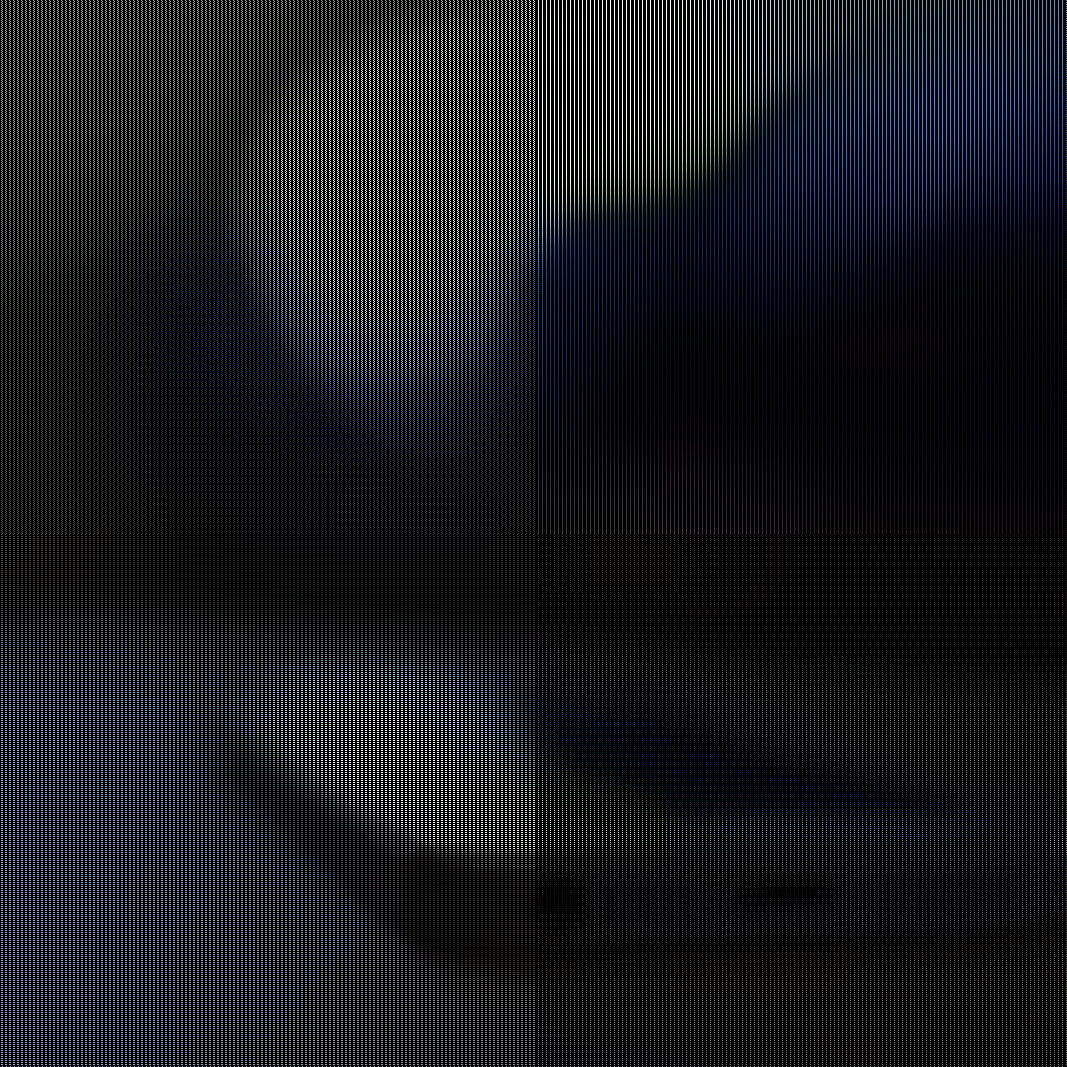
\includegraphics[width=8cm, height=8cm]{phone-without-interpolation.png}
	\end{center}
\end{figure}
\begin{figure}
	\caption{Przed uruchomieniem algorytmu (od lewej): obraz 1 (256x256, 300dpi), obraz 2 (256x256, 300dpi)}
	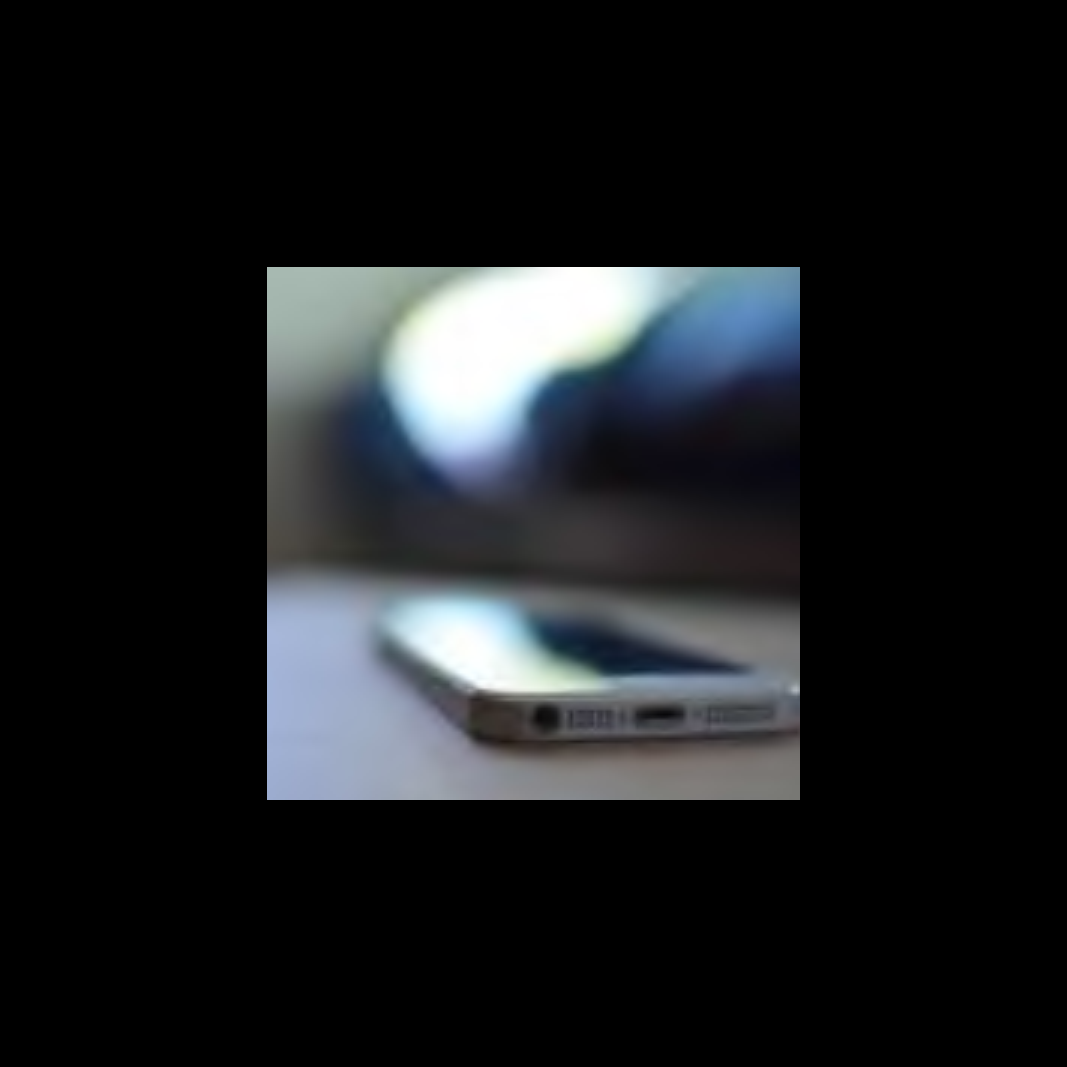
\includegraphics[width=8cm, height=8cm]{phone-geo-modified.png}
	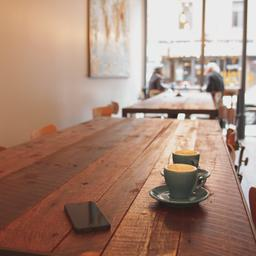
\includegraphics[width=8cm, height=8cm]{coffee-unmodified.jpg}
\end{figure}
\begin{figure}
	\caption{Po uruchomieniem algorytmu (od lewej): obraz 1 (256x256, 300dpi), obraz 2 (256x256, 300dpi)}
	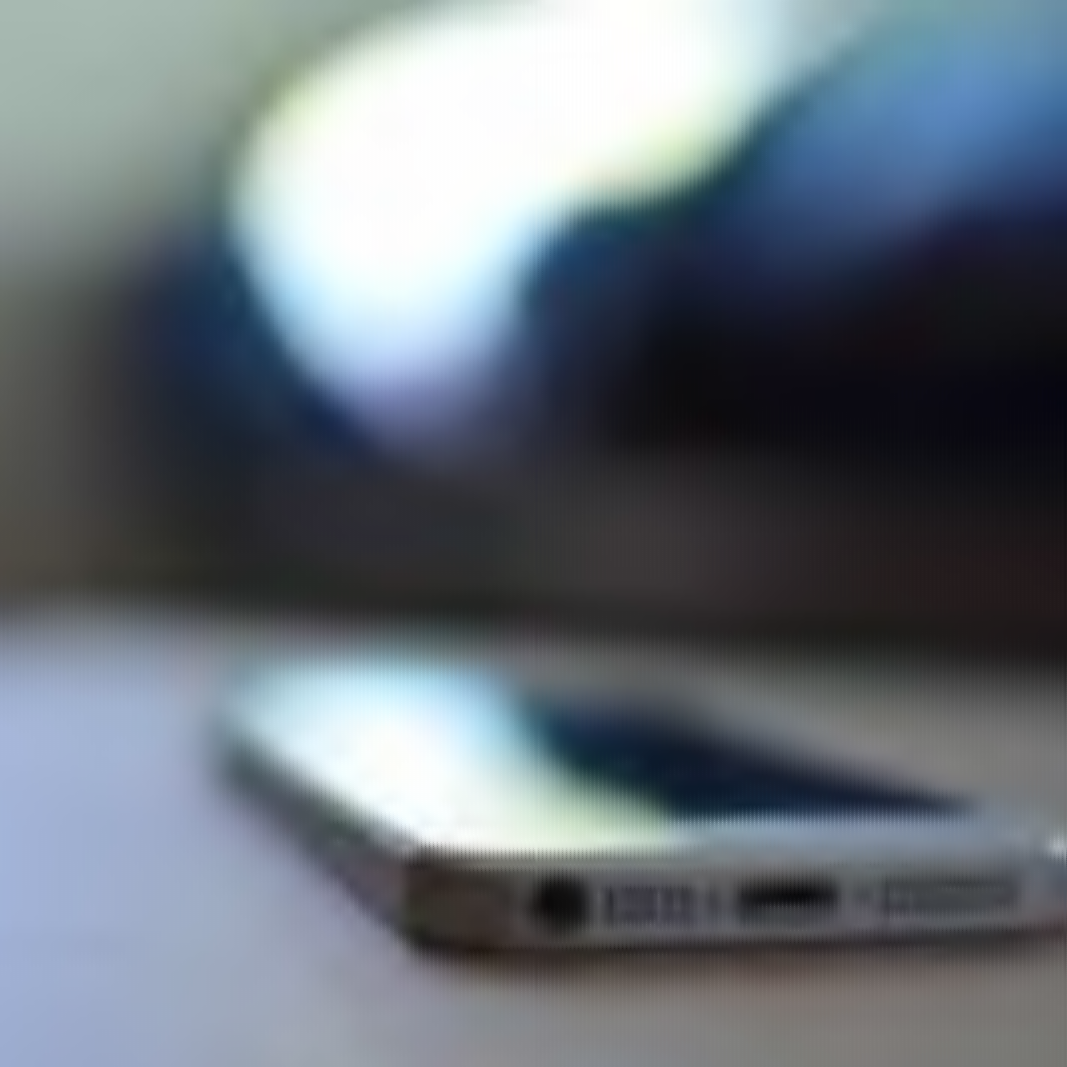
\includegraphics[width=8cm, height=8cm]{phone-rastar-unification.png}
	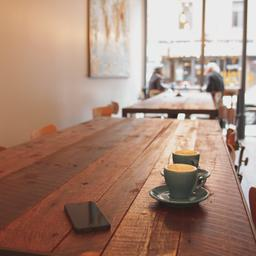
\includegraphics[width=8cm, height=8cm]{coffee-unmodified.jpg}
\end{figure}
\newpage
\subsection*{Kod źródłowy algorytmu}
\begin{python}
def rasterColor(self):
	print('rastar color unification start')
	self.firstDecoder.setColor()
	self._scaleUpColor(self.firstDecoder, 'Resources/rcUnification_1.png')
	print('first image done')
	self.secondDecoder.setColor()
	self._scaleUpColor(self.secondDecoder, 'Resources/rcUnification_2.png')
	print('second image done')
	print('rastar color unification done')

def _scaleUpColor(self, decoder, outputPath):
	width, height = decoder.width, decoder.height
	scaleFactoryW = float(self.maxWidth) / width
	scaleFactoryH = float(self.maxHeight) / height
	if width < self.maxWidth or height < self.maxHeight:
		pixelsBuffer = decoder.getPixels24Bits()
		result = numpy.full((self.maxHeight, self.maxWidth, 3), 1, numpy.uint8)
		# Fill values
		for h in range(height):
			for w in range(width):
				if w%2 == 0:
					result[int(scaleFactoryH * h), int(round(scaleFactoryW * w)) + 1] = pixelsBuffer[h, w]
				if w%2 == 1:
					result[int(round(scaleFactoryH * h)) + 1, int(scaleFactoryW * w)] = pixelsBuffer[h, w]
			# Interpolate
			self._interpolateColor(result)
			img = Image.fromarray(result, mode='RGB')
			img.save(outputPath)

def _interpolateColor(self, result):
	for h in range(self.maxHeight):
		for w in range(self.maxWidth):
			r, g, b = 0, 0, 0
			n = 0
			if (result[h, w][0] == 1) & (result[h, w][1] == 1) & (result[h, w][2] == 1):
				for hOff in range(-1, 2):
					for wOff in range(-1, 2):
						hSafe = h if ((h + hOff) > (self.maxHeight - 2)) | ((h + hOff) < 0) else (h + hOff)
						wSafe = w if ((w + wOff) > (self.maxWidth - 2)) | ((w + wOff) < 0) else (w + wOff)
						if (result[hSafe, wSafe][0] > 1) | (result[hSafe, wSafe][1] > 1) | (result[hSafe, wSafe][2] > 1):
							r += result[hSafe, wSafe][0]
							g += result[hSafe, wSafe][1]
							b += result[hSafe, wSafe][2]
							n += 1
				result[h, w] = (r/n, g/n, b/n)
\end{python}

\chapter{Operacje sumowania arytmetycznego obrazów szarych}
\section{Sumowanie (określonej) stałej z obrazem}
\section{Sumowanie dwóch obrazów}
\section{Mnożenie obrazu przez zadaną liczbę}
\section{Mnożenie obrazu przez inny obraz}
\section{Mieszanie obrazów z określonym współczynnikiem}
\section{Potęgowanie obrazu (z zadaną potęgą)}
\section{Dzielenie obrazu przez (zadaną) liczbę}
\section{Dzielenie obrazu przez przez inny obraz}
\section{Pierwiastkowanie obrazu}
\section{Logarytmowanie obrazu}

\chapter{Operacje sumowania arytmetycznego obrazów barwowych}
\section{Sumowanie (określonej) stałej z obrazem}
\section{Sumowanie dwóch obrazów}
\section{Mnożenie obrazu przez zadaną liczbę}
\section{Mnożenie obrazu przez inny obraz}
\section{Mieszanie obrazów z określonym współczynnikiem}
\section{Potęgowanie obrazu (z zadaną potęgą)}
\section{Dzielenie obrazu przez (zadaną) liczbę}
\section{Dzielenie obrazu przez przez inny obraz}
\section{Pierwiastkowanie obrazu}
\section{Logarytmowanie obrazu}

\chapter{Operacje geometryczne na obrazie}
Operacje geometryczne przekształcają położenie pikseli \textit{(x1, y1)} w obrazie wejściowym do nowej lokacji \textit{(x2, y2)} w obrazie wynikowym. Dzięki temu możemy dopasować obraz do odpowiedniego układu współrzędnych lub użyć tych operacji do eliminacji geometrycznych zakłóceń obrazu (dystorsji). 
\section{Przemieszczenie obrazu o zadany wektor}
\subsection*{Opis}
Operacja translacji wykonuje transformację geometryczną polegającą na przeniesieniu każdego z punktów obrazu wejściowego w nowe miejsce na obrazie wynikowym. Pod wpływem translacji element obrazu zlokalizowany na \textit{(x1, y1)} zostanie przesunięty na nową pozycję \textit{(x2, y2)}. Różnicą pomiędzy \textit{(x1, y1)} i \textit{(x2, y2)} jest wektor \textit{(bx, by)}, który jest określony przez użytkownika. 
\newline
Operacja przemieszczenia przybiera postać: 
\begin{gather}
	x_2 = x_1 + b_x \\
	y_2 = y_1 + b_y
\end{gather}
\begin{figure}[H]
	\caption{Przed uruchomieniem algorytmu (lewy obraz), po przesunięciu o wektor [100, 100] (prawy obraz)}
	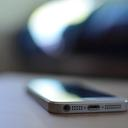
\includegraphics[width=8cm, height=8cm]{phone-unmodified.jpg}
	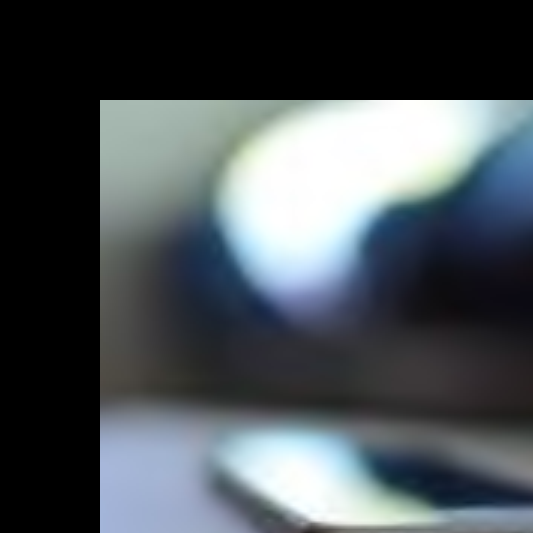
\includegraphics[width=8cm, height=8cm]{phone-translate.png}
\end{figure}
\begin{figure}[H]
	\caption{Przed uruchomieniem algorytmu (lewy obraz), po przesunięciu o wektor [100, -100] (prawy obraz)}
	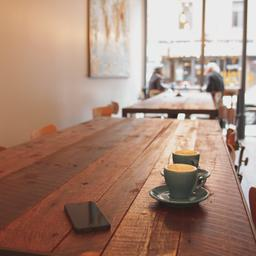
\includegraphics[width=8cm, height=8cm]{coffee-unmodified.jpg}
	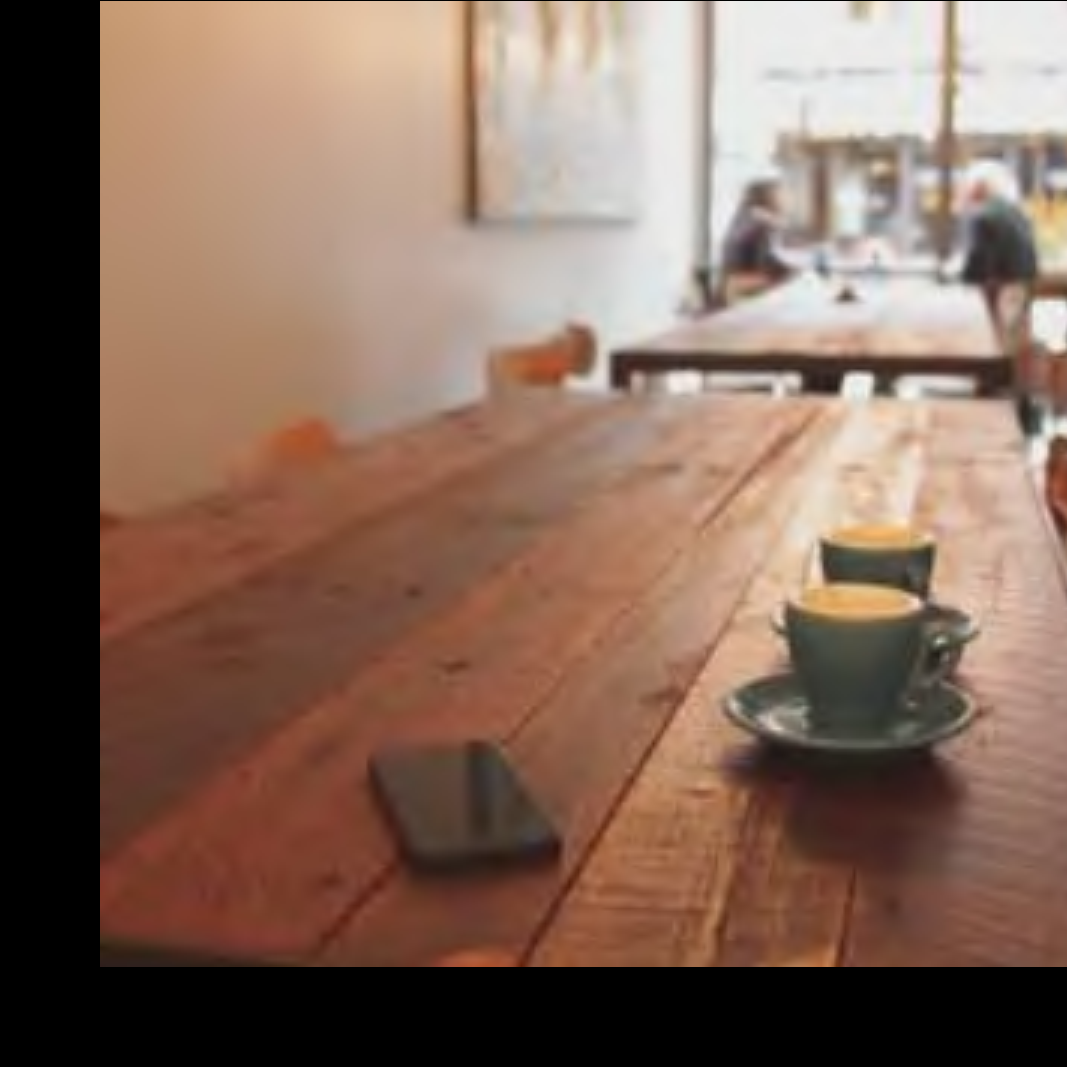
\includegraphics[width=8cm, height=8cm]{coffee-translate.png}
\end{figure}
\subsection*{Kod źródłowy algorytmu}
\begin{python}
def translate(self, deltaX = 0, deltaY = 0):
	print('translation start')
	height, width = self.decoder.height, self.decoder.width
	image = self.decoder.getPixels24Bits()
	result = numpy.zeros((height, width, 3), numpy.uint8)
	
	for y in range(height):
		for x in range(width):  
			if 0 < y + deltaY < height and 0 < x + deltaX < width:
				result[y + deltaY][x + deltaX] = image[y][x]
	
	img = Image.fromarray(result, mode='RGB')
	img.save('Resources/tGeometric.png')
print('translation done')
\end{python}
\section{Jednorodne skalowanie obrazu}
\subsection*{Opis}
Skalowanie jednorodne obrazu składa się na pomnożenie współrzędnych każdego piksela przez określoną wartość. 
\begin{gather}
x_2 = S_x * x_1 \\
y_2 = S_y * y_1
\end{gather}
Przy czym skalowanie jednorodne oznacza, że po zmianie wartości współrzędnych nasz obraz zachowa dawne proporcje. Czyli: 
\begin{gather}
S_x = S_y
\end{gather}
\begin{figure}[H]
	\caption{Przed uruchomieniem algorytmu (lewy obraz), po skalowaniu jednorodnym o współczynnik 2 (prawy obraz)}
	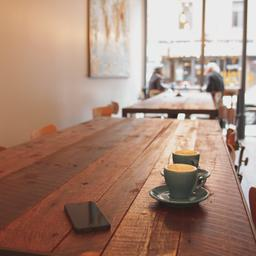
\includegraphics[width=4cm, height=4cm]{coffee-unmodified.jpg}
	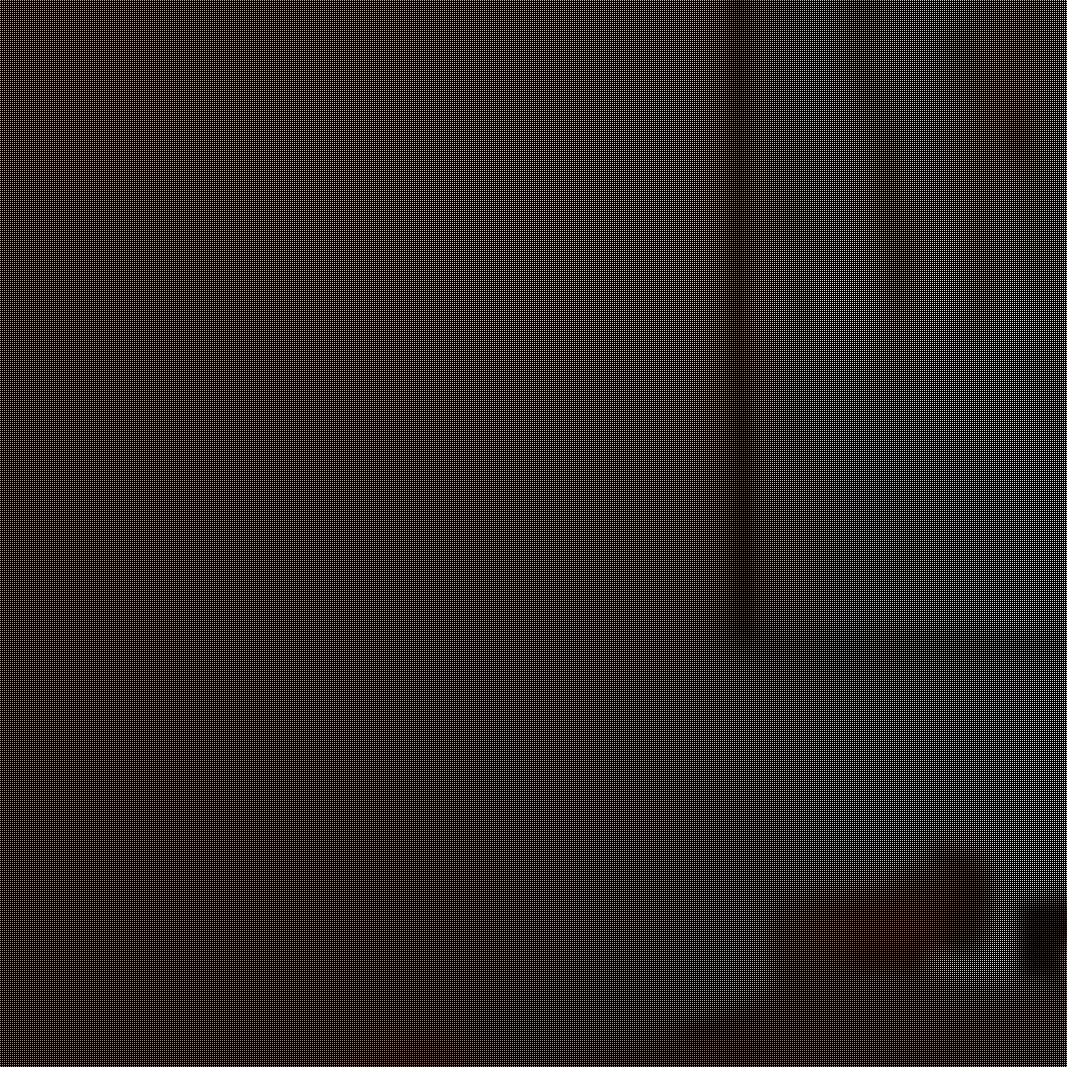
\includegraphics[width=4cm, height=4cm]{coffee-hscaling-without-interpolation.png}
	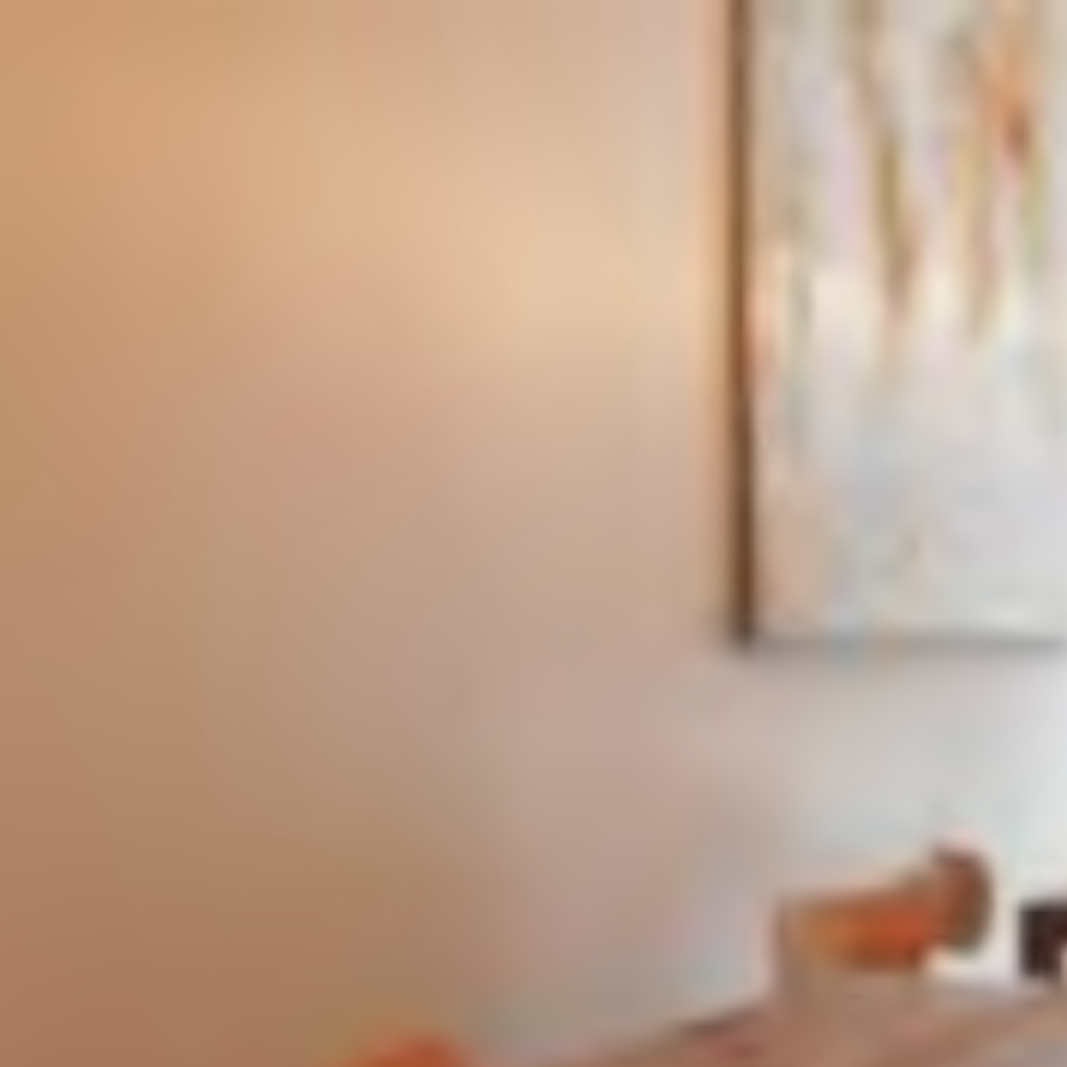
\includegraphics[width=4cm, height=4cm]{coffee-hscaling.png}
\end{figure}
\subsection*{Kod źródłowy algorytmu}
\begin{python}
def homogeneousScaling(self, scale = 1.0):
	print('homogeneous scaling start')
	image = self.decoder.getPixels24Bits()
	
	print('scaling')
	result = self._scaleXY(image, scale)
	print('interpolation')
	self._interpolateColor(result)
	
	img = Image.fromarray(result, mode='RGB')
	img.save('Resources/hsGeometric.png')
	print('homogeneous scaling done')

def _scaleXY(self, matrix, scale):
	height, width = self.decoder.height, self.decoder.width
	result = numpy.full((height, width, 3), 1, numpy.uint8)
	for y in range(height):
		for x in range(width):  
			if scale * y < height and scale * x < width:
				result[int(scale * y)][int(scale * x)] = matrix[y][x]
	return result

def _interpolateColor(self, result):
	height, width = self.decoder.height, self.decoder.width
	for h in range(height):
		for w in range(width):
			r, g, b = 0, 0, 0
			n = 0
			if (result[h, w][0] == 1) & (result[h, w][1] == 1) & (result[h, w][2] == 1):
				for hOff in range(-1, 2):
					for wOff in range(-1, 2):
						hSafe = h if ((h + hOff) > (height - 2)) | ((h + hOff) < 0) else (h + hOff)
						wSafe = w if ((w + wOff) > (width - 2)) | ((w + wOff) < 0) else (w + wOff)
						if (result[hSafe, wSafe][0] > 1) | (result[hSafe, wSafe][1] > 1) | (result[hSafe, wSafe][2] > 1):
							r += result[hSafe, wSafe][0]
							g += result[hSafe, wSafe][1]
							b += result[hSafe, wSafe][2]
							n += 1
				result[h, w] = (r/n, g/n, b/n)
\end{python}
\section{Niejednorodne skalowanie obrazu}
\subsection*{Opis}
Skalowanie niejednorodne obrazu składa się na pomnożenie współrzędnych każdego piksela przez określoną wartość. 
\begin{gather}
x_2 = S_x * x_1 \\
y_2 = S_y * y_1
\end{gather}
Przy czym skalowanie niejednorodne oznacza, że po zmianie wartości współrzędnych nasz obraz będzie miał zachwiane proporcje. Czyli: 
\begin{gather}
S_x \neq S_y
\end{gather}
\begin{figure}[H]
	\caption{Przed uruchomieniem algorytmu (lewy obraz), po skalowaniu jednorodnym o współczynnik x = 2.0, y = 1.0 (prawy obraz)}
	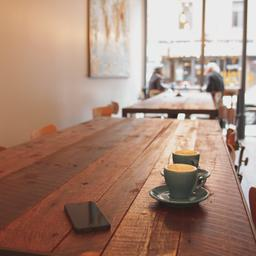
\includegraphics[width=4cm, height=4cm]{coffee-unmodified.jpg}
	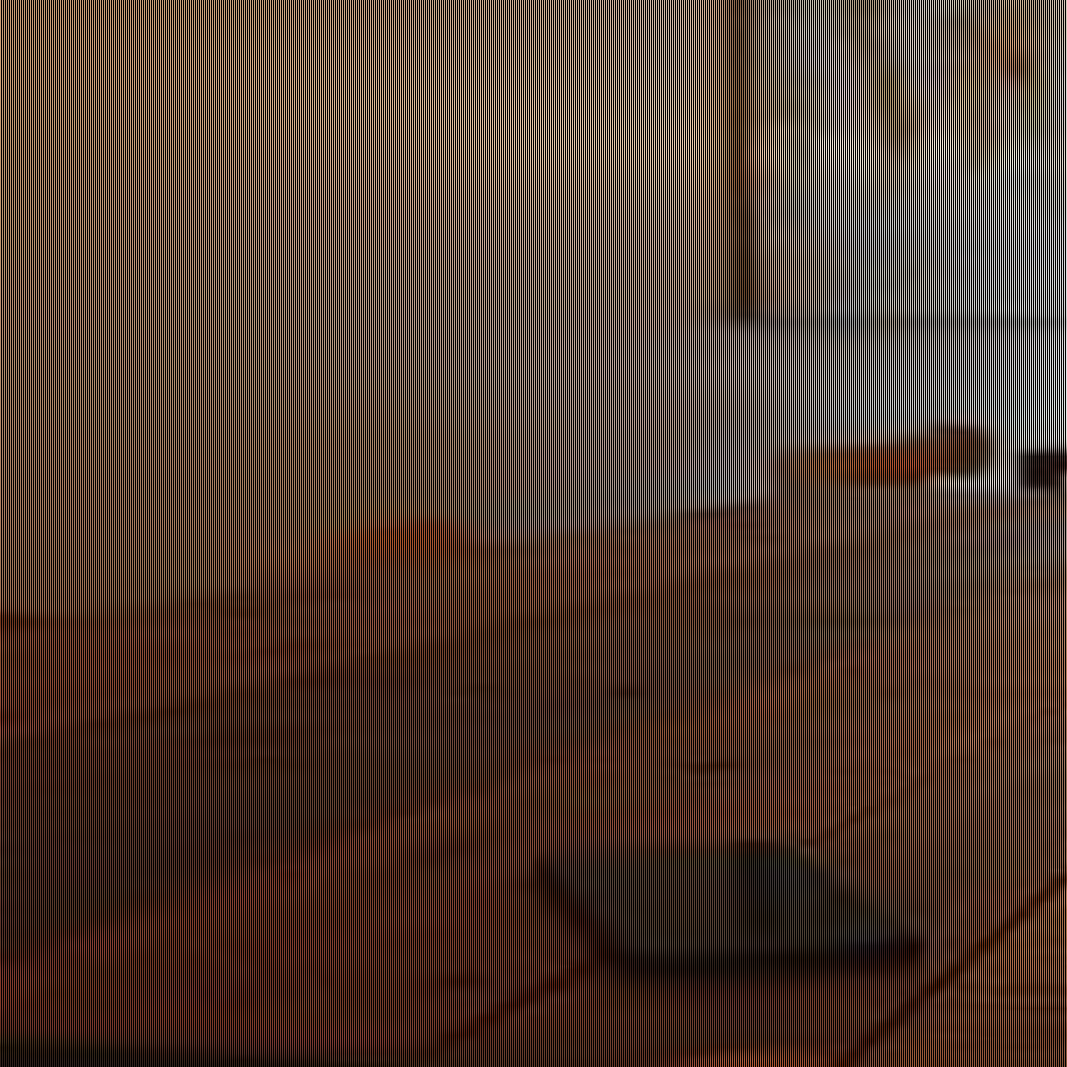
\includegraphics[width=4cm, height=4cm]{coffee-nonuniform-scaling-without-interpolation.png}
	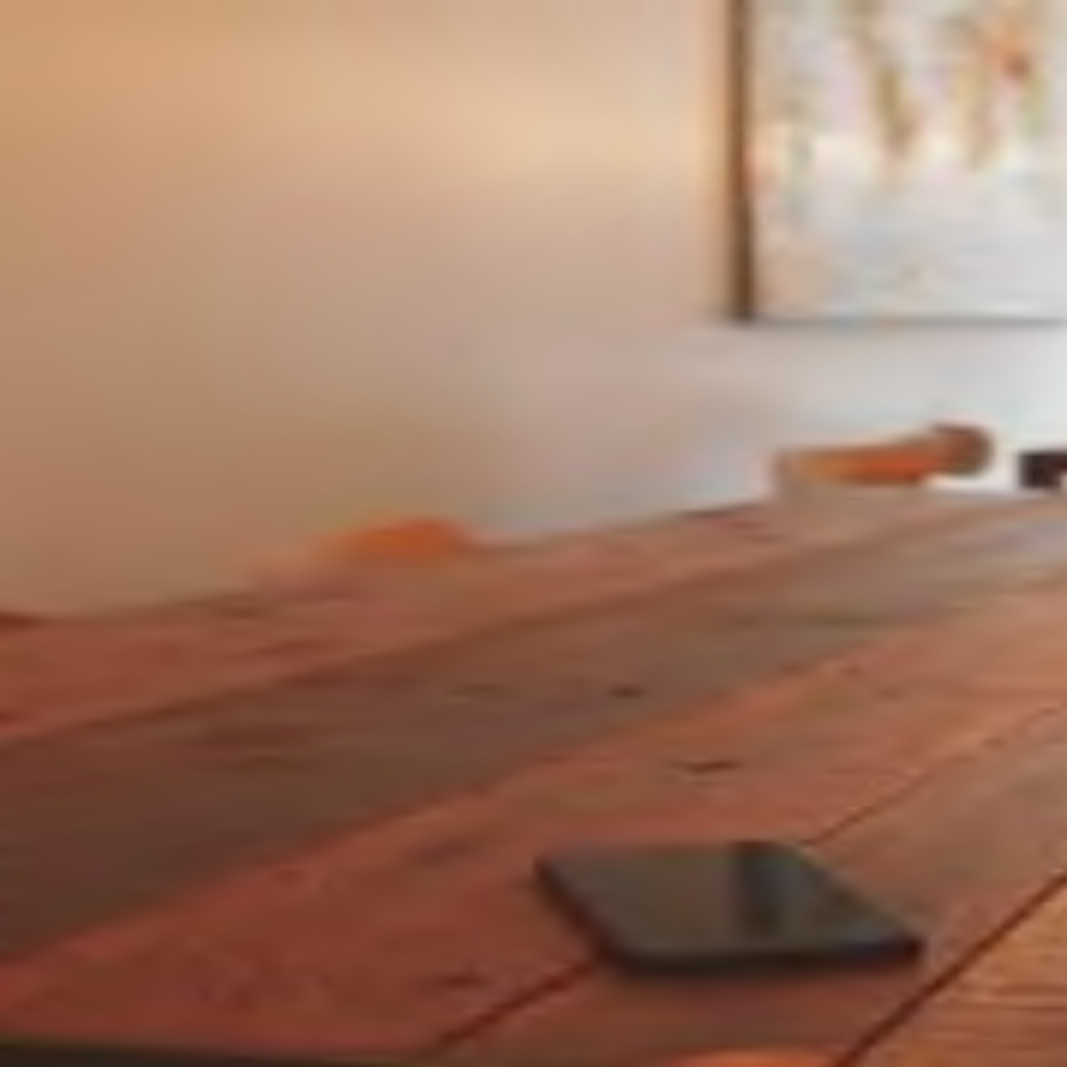
\includegraphics[width=4cm, height=4cm]{coffee-nonuniform-scaling.png}
\end{figure}
\subsection*{Kod źródłowy algorytmu}
\begin{python}
def nonUniformScaling(self, scaleX = 1.0, scaleY = 1.0):
	print('non-uniform scaling start')
	image = self.decoder.getPixels24Bits()
	
	print('scaling')
	result = self._scale(image, scaleX, scaleY)
	print('interpolation')
	self._interpolateColor(result)
	
	img = Image.fromarray(result, mode='RGB')
	img.save('Resources/nusGeometric.png')
	print('non-uniform scaling done')

def _scale(self, matrix, scaleX, scaleY):
	height, width = self.decoder.height, self.decoder.width
	result = numpy.full((height, width, 3), 1, numpy.uint8)
	for y in range(height):
		for x in range(width):  
			if scaleY * y < height and scaleX * x < width:
				result[int(scaleY * y)][int(scaleX * x)] = matrix[y][x]
	return result

def _interpolateColor(self, result):
	height, width = self.decoder.height, self.decoder.width
	for h in range(height):
		for w in range(width):
			r, g, b = 0, 0, 0
			n = 0
				if (result[h, w][0] == 1) & (result[h, w][1] == 1) & (result[h, w][2] == 1):
					for hOff in range(-1, 2):
						for wOff in range(-1, 2):
							hSafe = h if ((h + hOff) > (height - 2)) | ((h + hOff) < 0) else (h + hOff)
							wSafe = w if ((w + wOff) > (width - 2)) | ((w + wOff) < 0) else (w + wOff)
							if (result[hSafe, wSafe][0] > 1) | (result[hSafe, wSafe][1] > 1) | (result[hSafe, wSafe][2] > 1):
								r += result[hSafe, wSafe][0]
								g += result[hSafe, wSafe][1]
								b += result[hSafe, wSafe][2]
								n += 1
						result[h, w] = (r/n, g/n, b/n)
\end{python}
\section{Obracanie obrazu o dowolny kąt}
\subsection*{Opis}
Operacja obrotu wykonywana jest wokół początku układu współrzędnych o kąt $\varphi$ w taki sposób aby odległość od początku układu do punktu pozostała bez zmian, oraz aby pomiędzy odcinkami danych punków był kąt $\varphi$. Właściwości te można pozyskać dzięki wzorom: 
\begin{gather}
	x` = x\cos(\varphi) - y\sin(\varphi) \\
	y` = x\sin(\varphi) + y\cos(\varphi)
\end{gather}
gdzie \textit{(x`, y`)} to nowe współrzędne wyznaczone po obrocie punktu \textit{(x, y)} o kąt $\varphi$. 
\begin{figure}[H]
	\caption{Przed uruchomieniem algorytmu (lewy obraz), po obróceniu o kąt $45^o$(prawy obraz), po obrocie bez interpolacji (środkowy obraz)}
	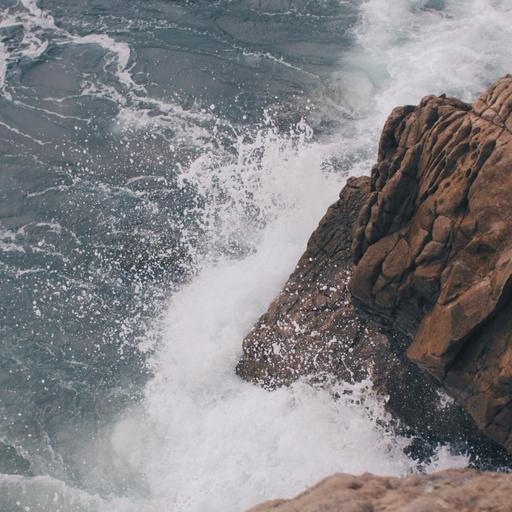
\includegraphics[width=4cm, height=4cm]{sea-unmodified.jpg}
	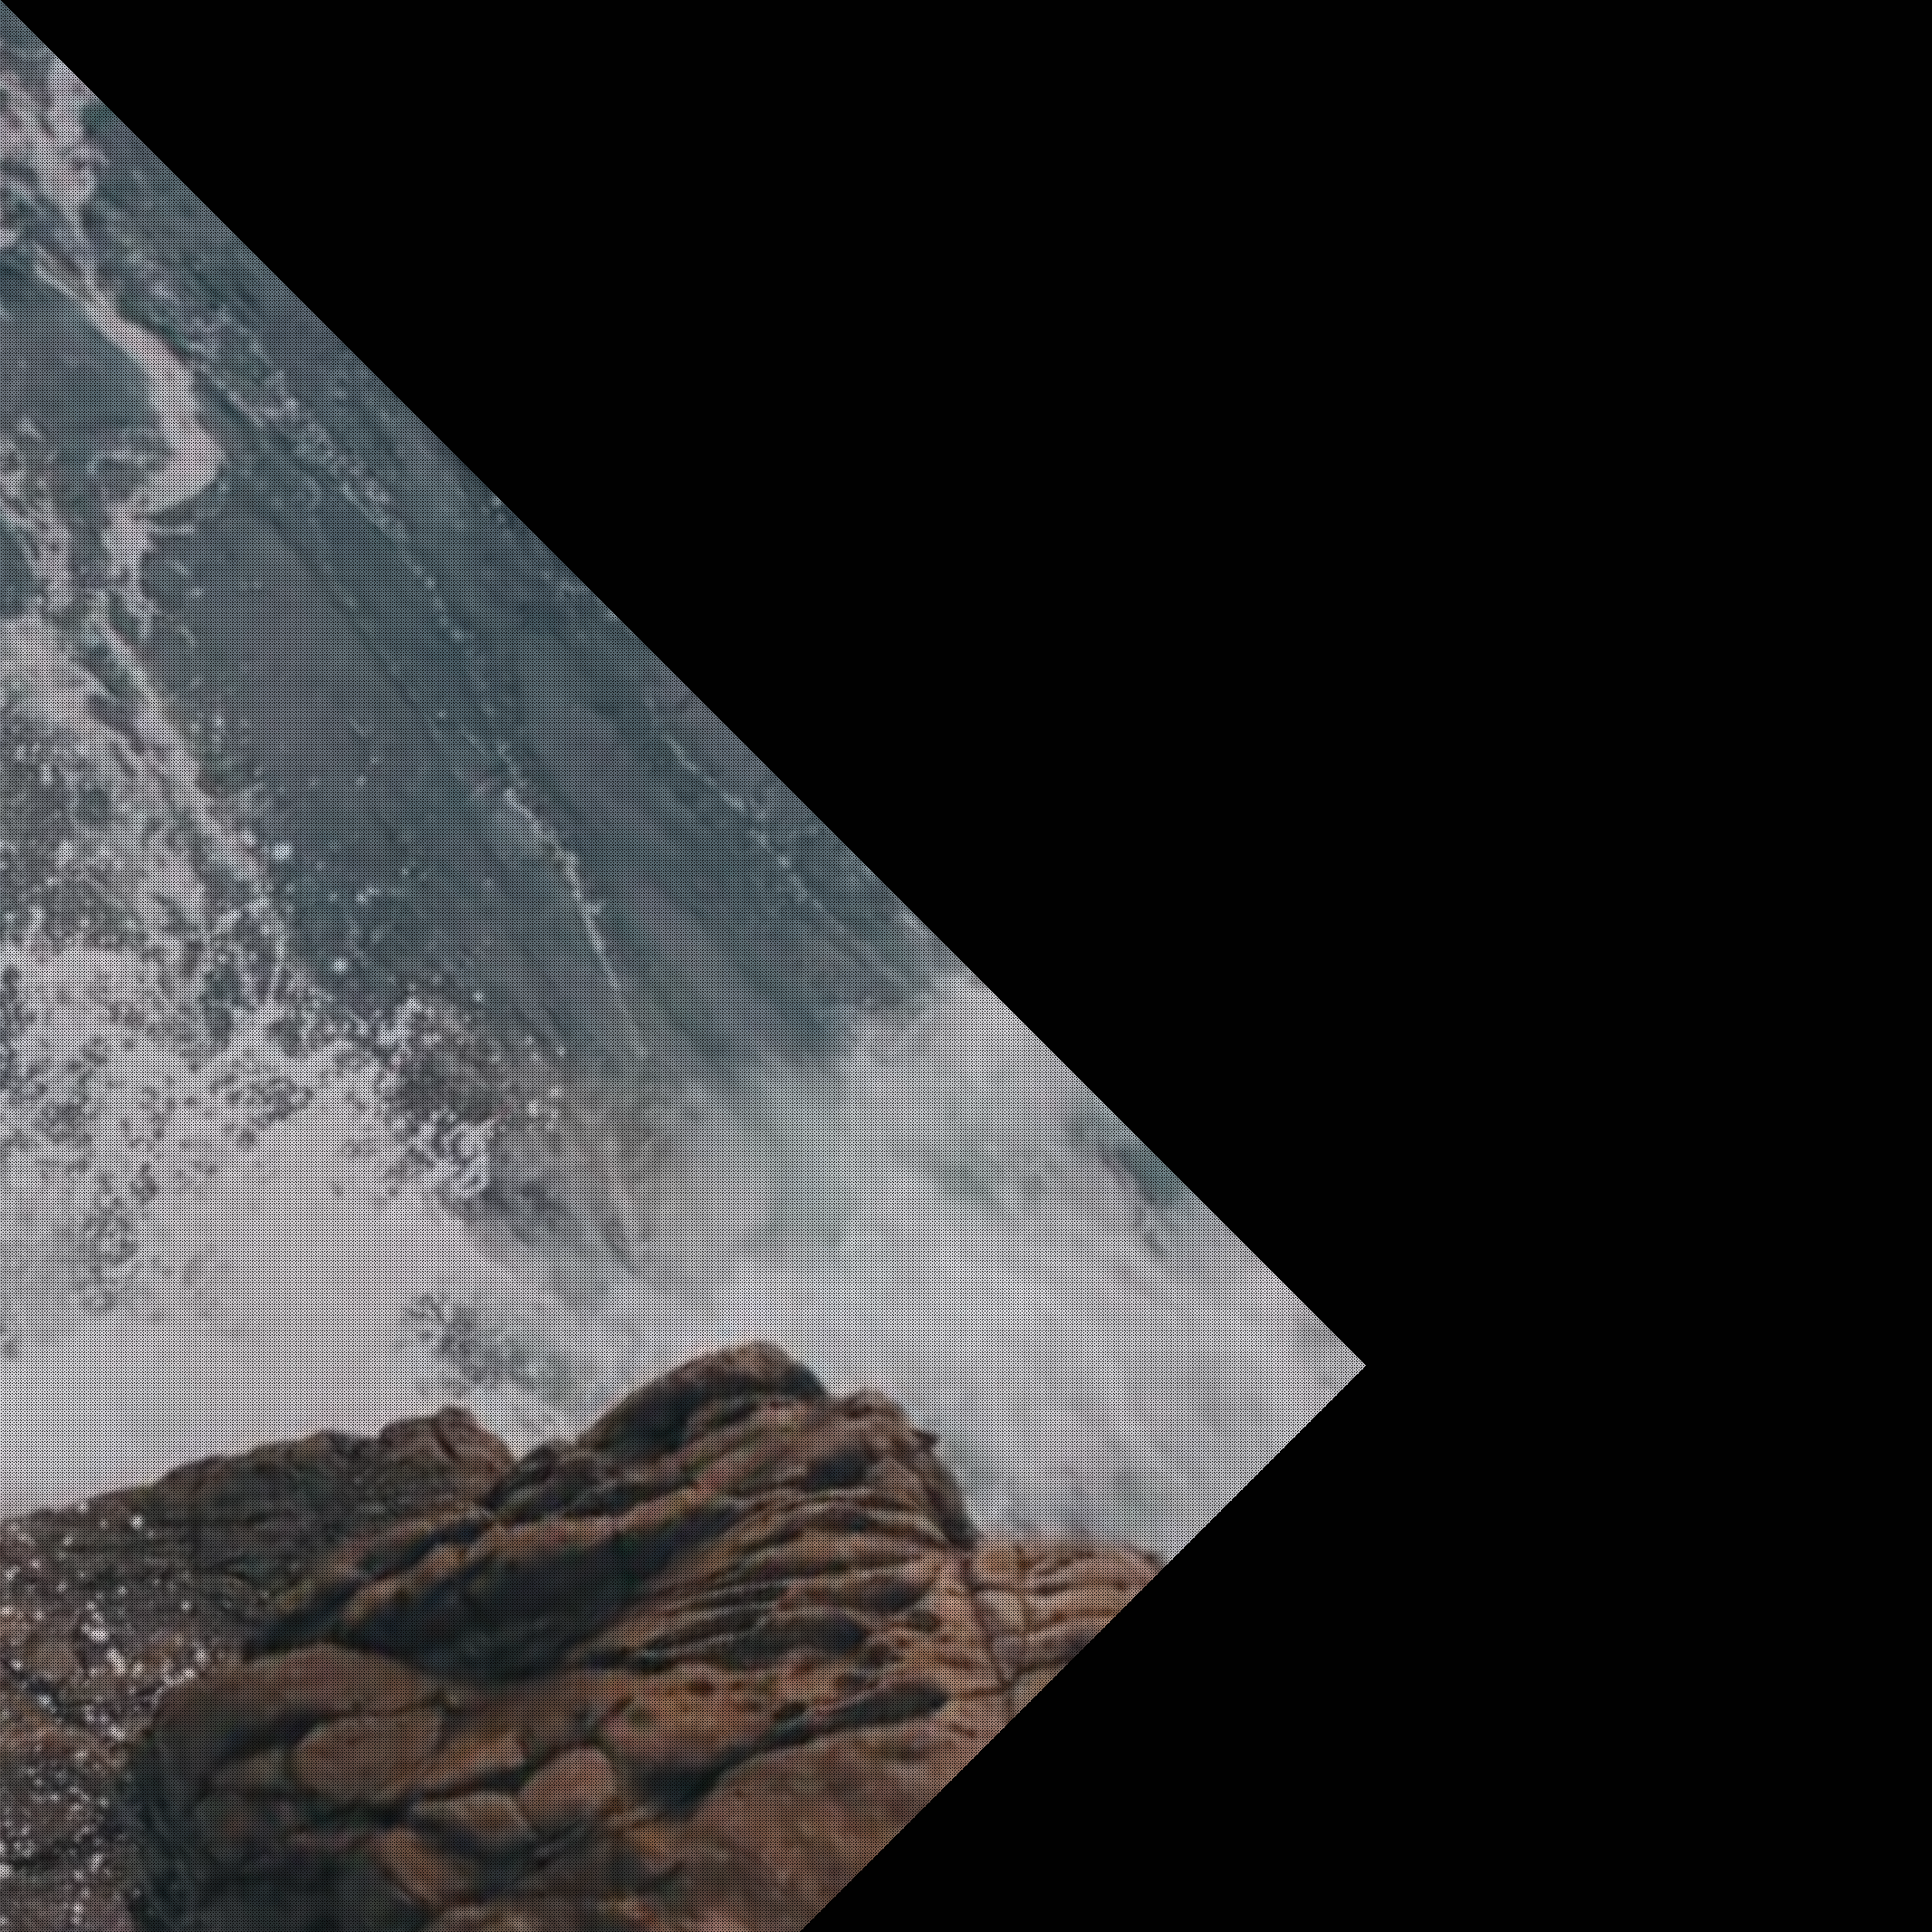
\includegraphics[width=4cm, height=4cm]{sea-rotation-without-interpolation.png}
	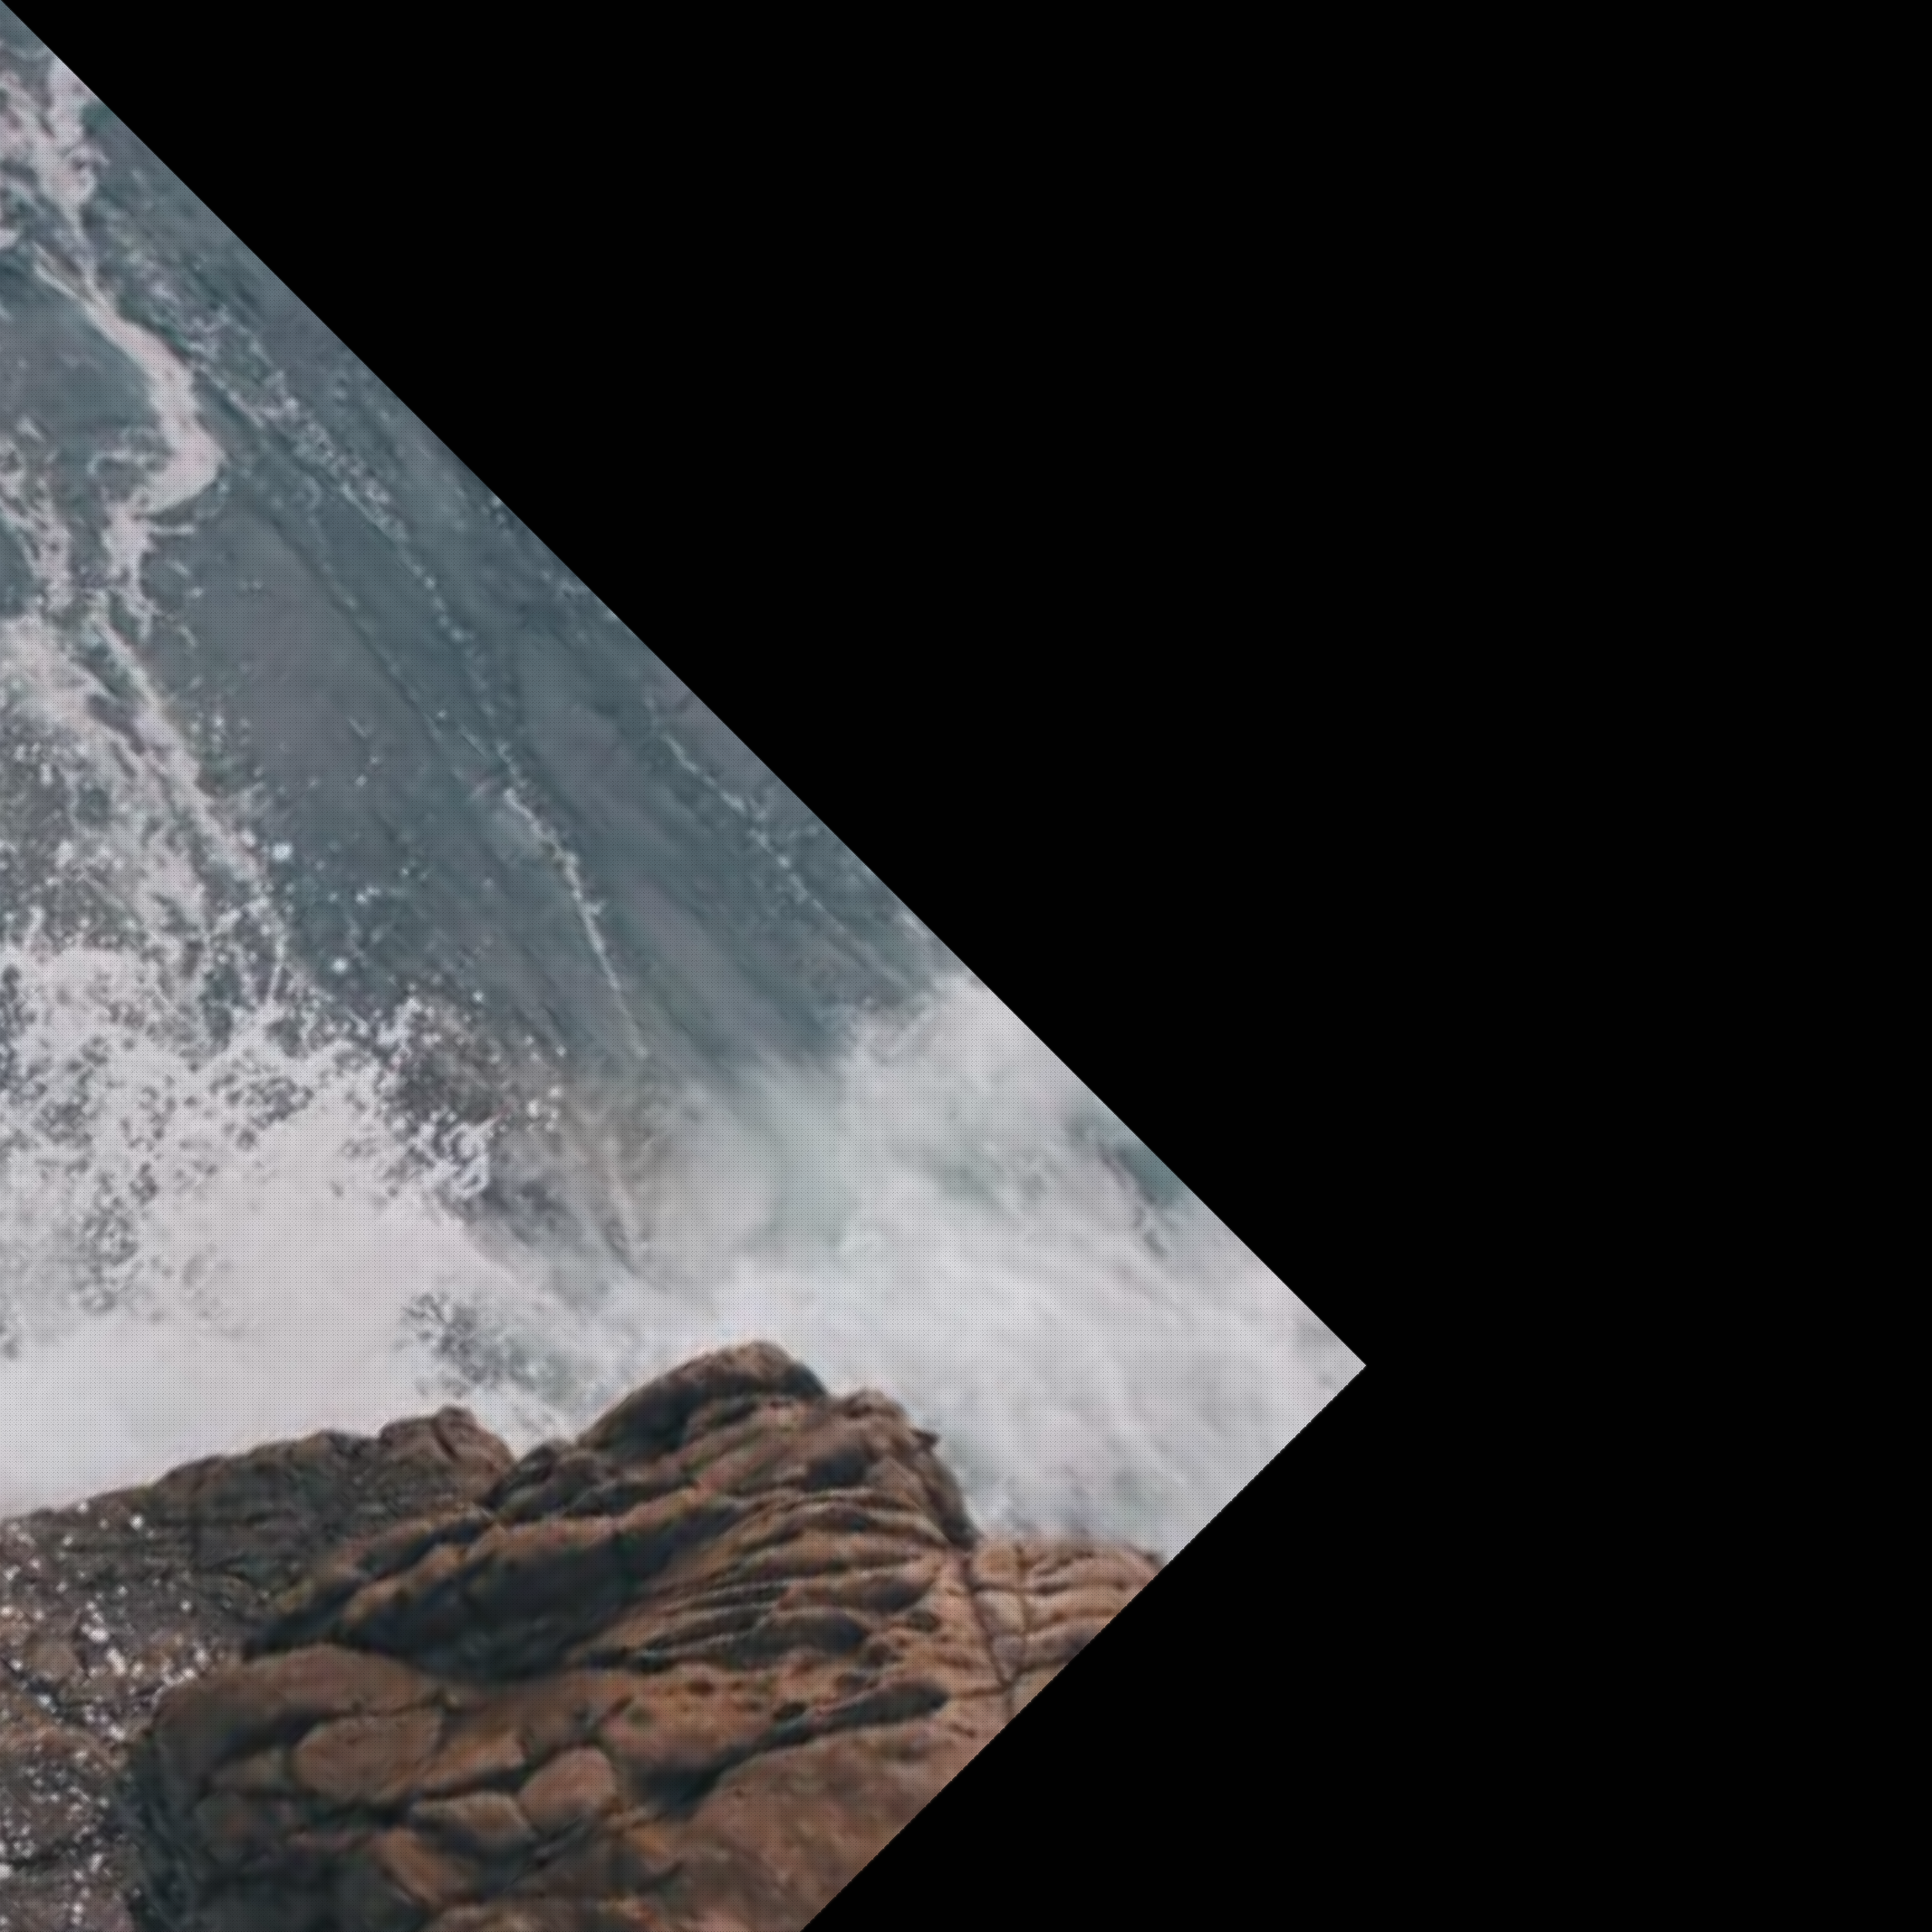
\includegraphics[width=4cm, height=4cm]{sea-rotation.png}
\end{figure}
\subsection*{Kod źródłowy algorytmu}
\begin{python}
def rotation(self, phi):
	print('rotation start')
	image = self.decoder.getPixels24Bits()
	
	print('rotating')
	result = self._rotate(image, phi)
	print('interpolation')
	self._interpolateColor(result)
	
	img = Image.fromarray(result, mode='RGB')
	img.save('Resources/rGeometric.png')
	print('rotation done')

def _rotate(self, image, phi):
	height, width = self.decoder.height, self.decoder.width
	result = numpy.full((height, width, 3), 1, numpy.uint8)
	radian = math.radians(phi)
	for y in range(height):
		for x in range(width): 
			newX = x*math.cos(radian) - y*math.sin(radian)
			newY = x*math.sin(radian) + y*math.cos(radian)
			if newY < height and newY >= 0 and newX >= 0 and newX < width:
				result[int(newY)][int(newX)] = image[y][x]
	return result

def _interpolateColor(self, result):
	height, width = self.decoder.height, self.decoder.width
	for h in range(height):
		for w in range(width):
			r, g, b = 0, 0, 0
			n = 0
			if (result[h, w][0] == 1) & (result[h, w][1] == 1) & (result[h, w][2] == 1):
				for hOff in range(-1, 2):
					for wOff in range(-1, 2):
						hSafe = h if ((h + hOff) > (height - 2)) | ((h + hOff) < 0) else (h + hOff)
						wSafe = w if ((w + wOff) > (width - 2)) | ((w + wOff) < 0) else (w + wOff)
						if (result[hSafe, wSafe][0] > 0) | (result[hSafe, wSafe][1] > 0) | (result[hSafe, wSafe][2] > 0):
							r += result[hSafe, wSafe][0]
							g += result[hSafe, wSafe][1]
							b += result[hSafe, wSafe][2]
							n += 1
				result[h, w] = (r/n, g/n, b/n)
\end{python}
\section{Symetrie względem osi układu}
\subsection*{Opis}
Symetria osiowa względem osi OX lub OY sprawia, że punkt \textit{(x, y)} zmienia się w \textit{(x, -y)} lub \textit{(-x, y)} w zależności czy symetria dotyczyła osi OX lub OY. W naszej pracy przyjmujemy, że lewa dolna krawędź obrazu znajduje się w punkcie \textit{(0, 0)}. 
\begin{figure}[H]
	\caption{Od lewej: przed uruchomieniem algorytmu, po symetrii względem OX, po symetrii względem OY, po symetrii względem OX oraz OY}
	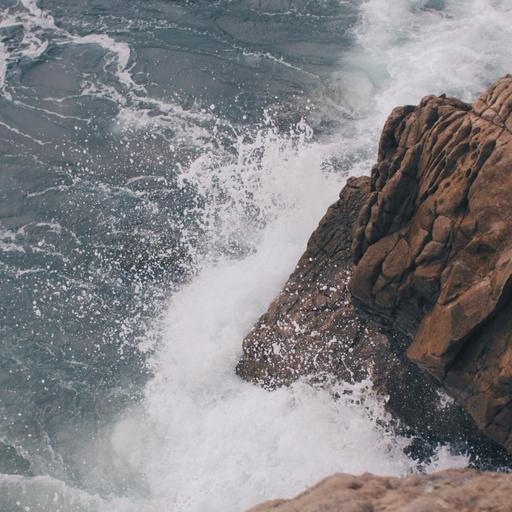
\includegraphics[width=7cm, height=7cm]{sea-unmodified.jpg}
	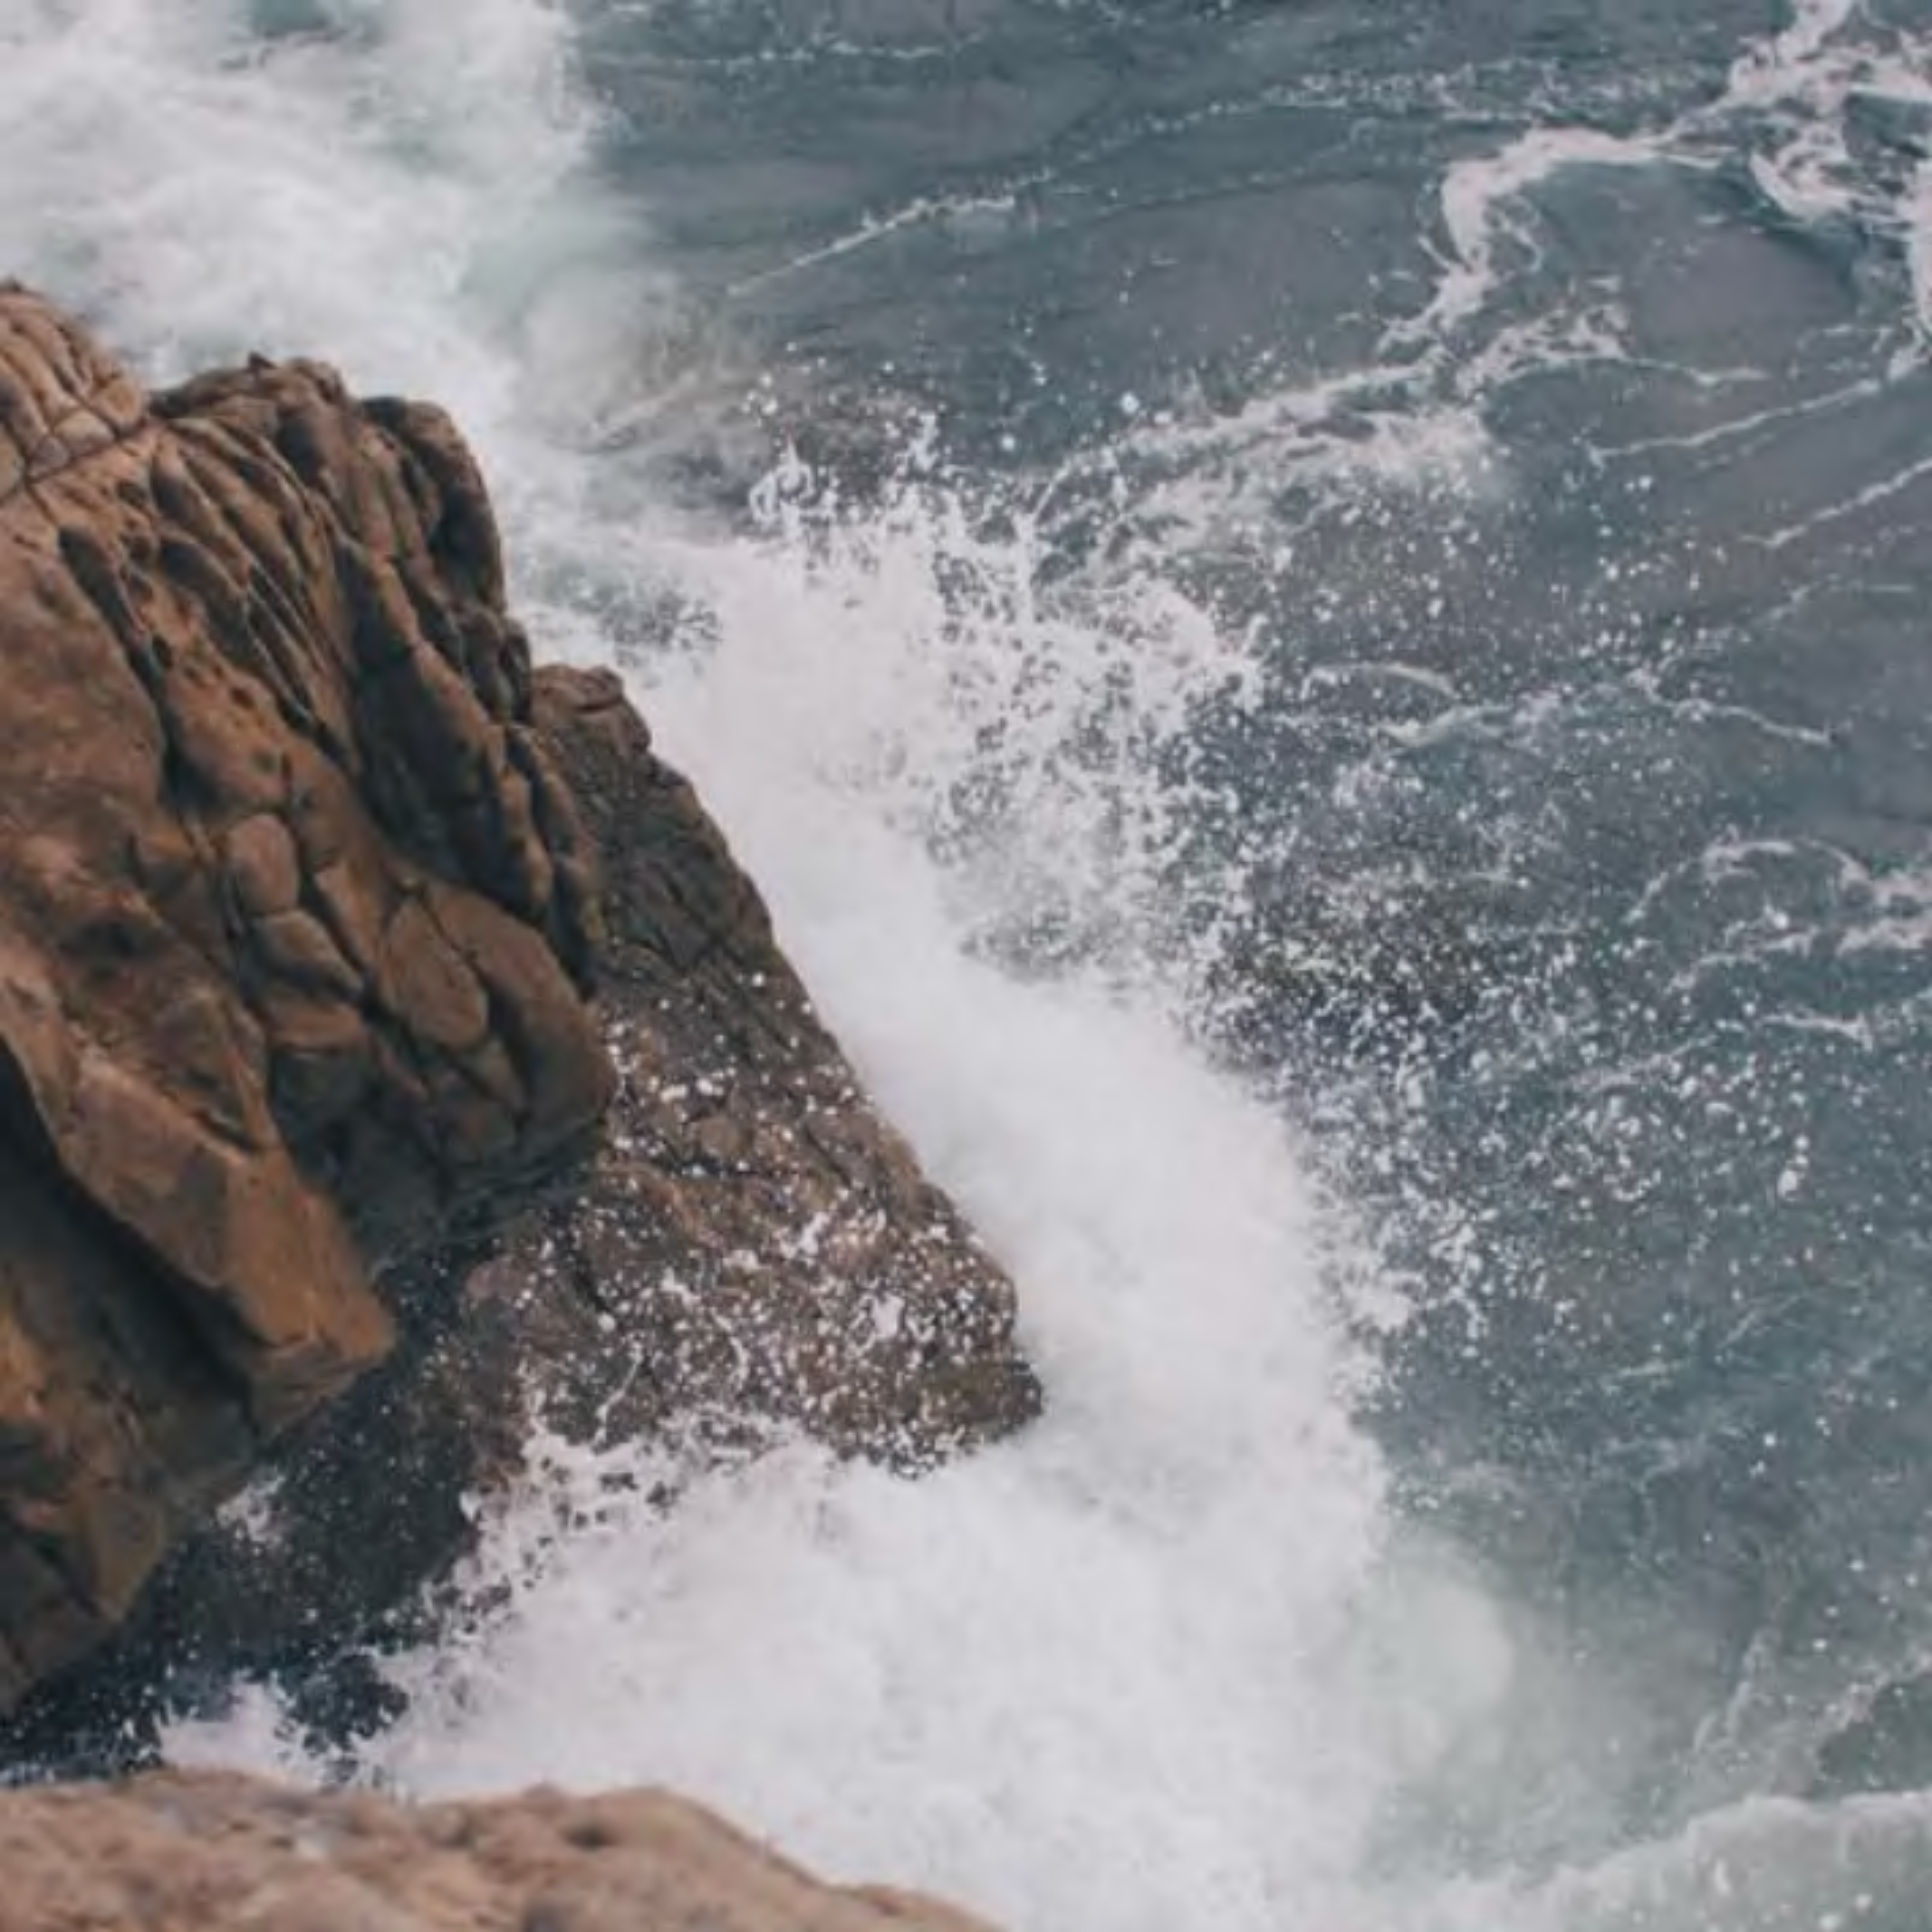
\includegraphics[width=7cm, height=7cm]{sea-symmetry-x.png}
	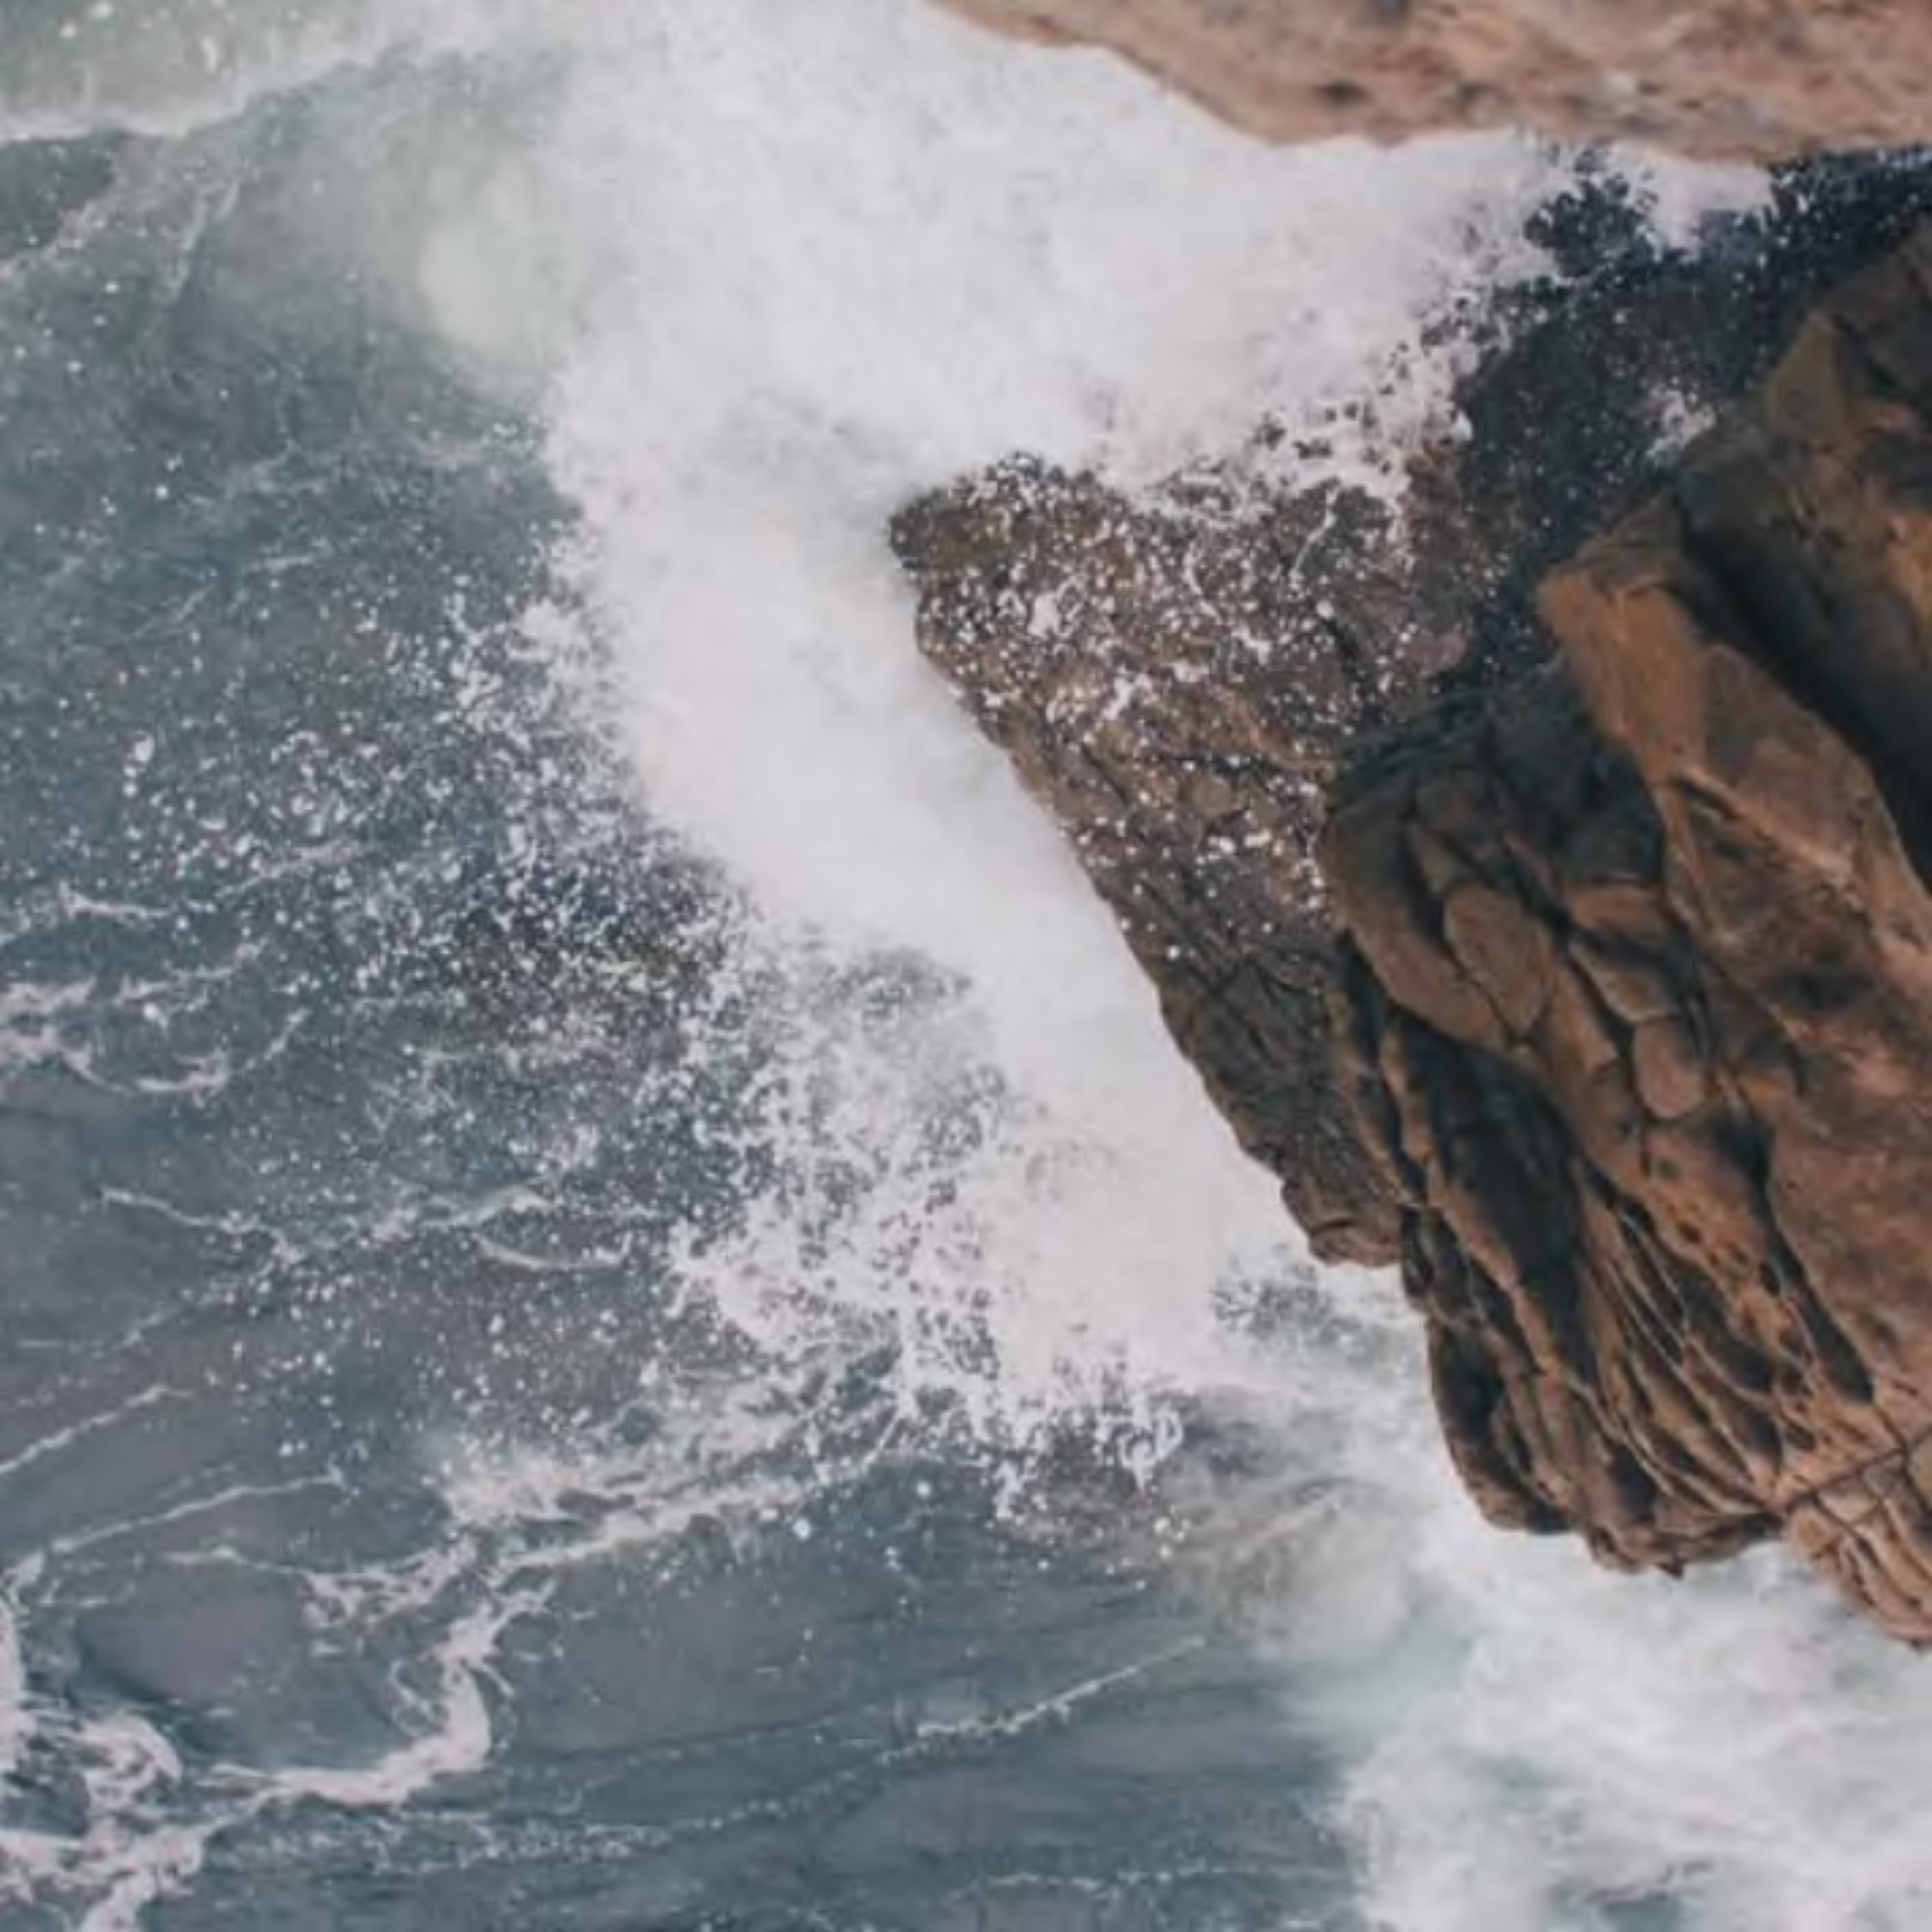
\includegraphics[width=7cm, height=7cm]{sea-symmetry-y.png}
	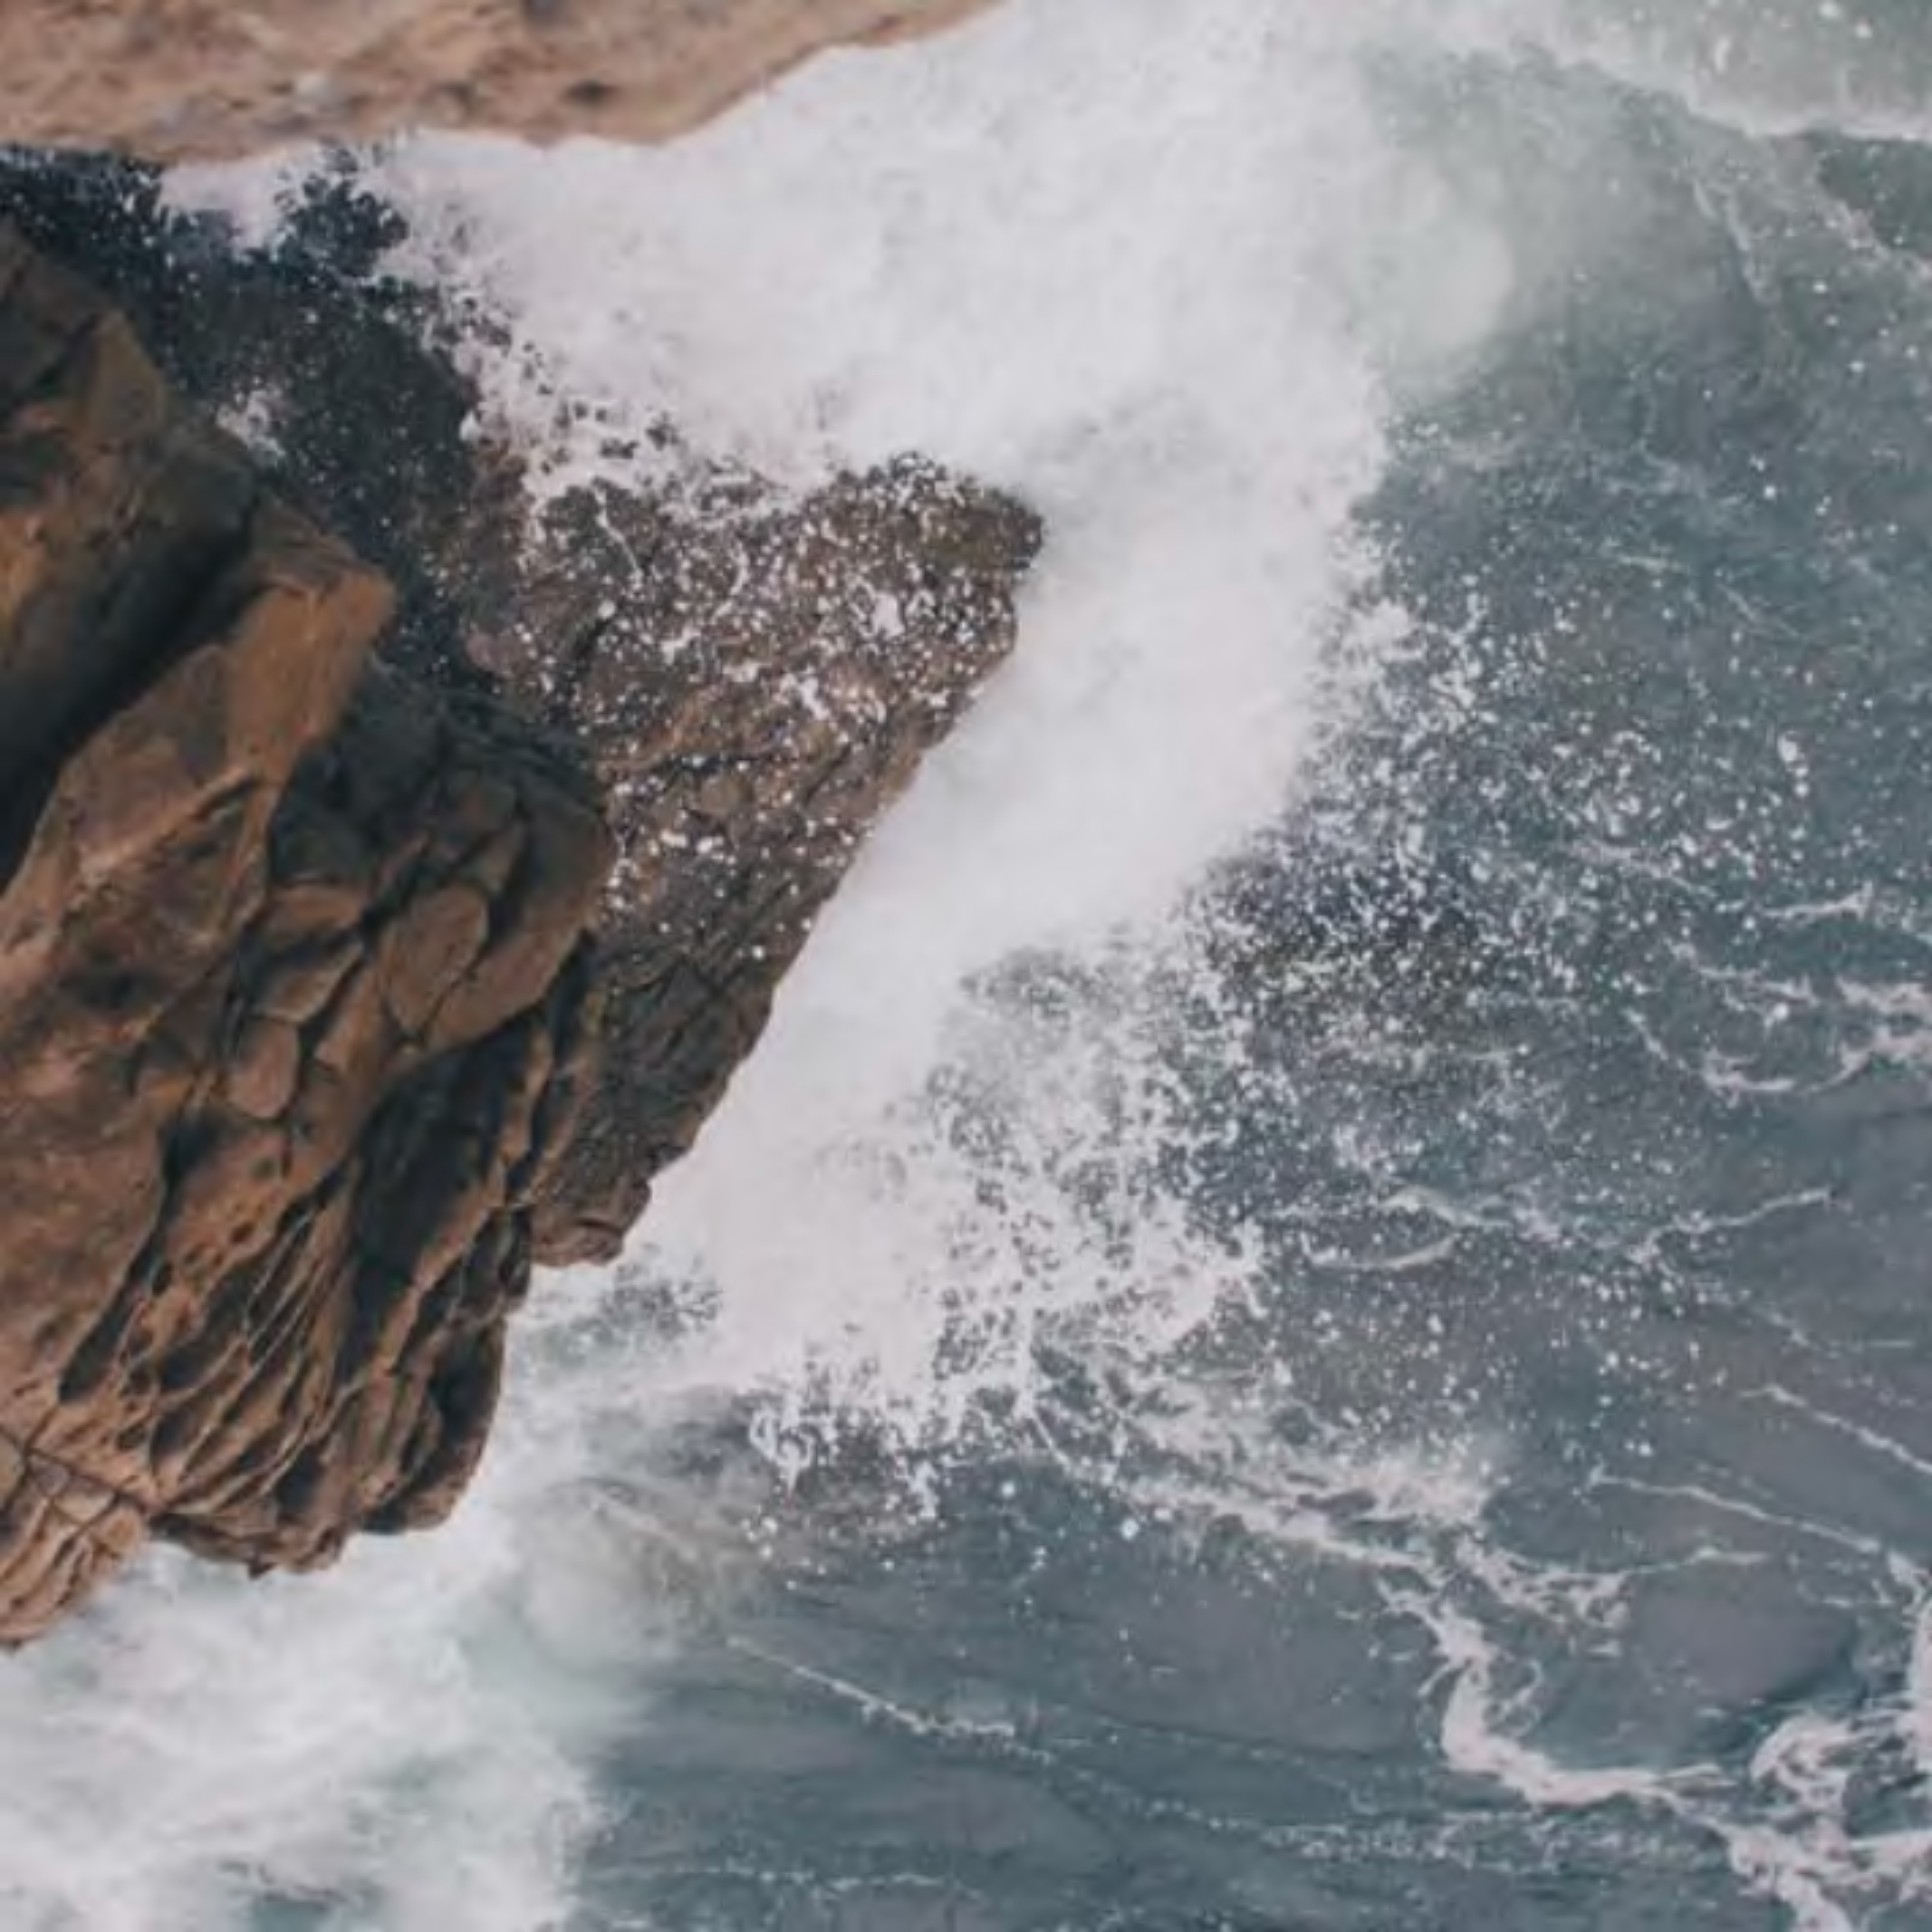
\includegraphics[width=7cm, height=7cm]{sea-symmetry-xy.png}
\end{figure}
\subsection*{Kod źródłowy algorytmu}
\begin{python}
def axisSymmetry(self, ox, oy):
	print('axis symmetry start')
	image = self.decoder.getPixels24Bits()
	
	print('symmetry operation')
	result = self._symmetryOXorOY(image, ox, oy)
	
	img = Image.fromarray(result, mode='RGB')
	img.save('Resources/Geometric-AxisSymmetry.png')
	print('axis symmetry done')

def _symmetryOXorOY(self, image, ox, oy):
	height, width = self.decoder.height, self.decoder.width
	result = numpy.zeros((height, width, 3), numpy.uint8)
	for y in range(height):
		for x in range(width): 
			if ox and not oy:
				result[y][x] = image[y][(width-1)-x]
			elif not ox and oy:
				result[y][x] = image[(height-1)-y][x]
			elif ox and oy:
				result[y][x] = image[(height-1)-y][(width-1)-x]
	return result
\end{python}
\section{Symetrie względem zadanej prostej}
\subsection*{Opis}
Przypadek podobny do poprzedniego, lecz tym razem użytkownik podaje wiersz lub kolumnę względem której będzie przebiegała oś symetrii. 
\begin{figure}[H]
	\caption{Przed uruchomieniem algorytmu (lewy), po symetrii względem prostej \textit{x=356} (środkowy), po symetrii względem prostej \textit{y=356} (prawy)}
	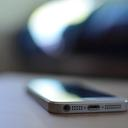
\includegraphics[width=4cm, height=4cm]{phone-unmodified.jpg}
	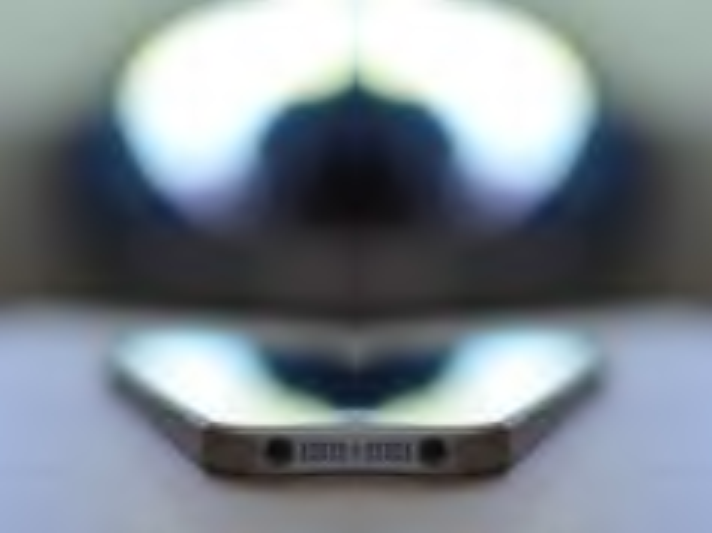
\includegraphics[width=4cm, height=4cm]{phone-custom-symmetry-x.png}
	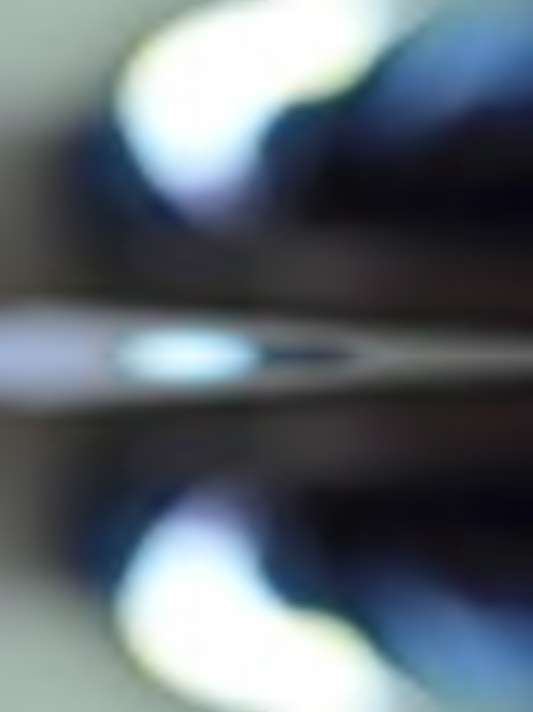
\includegraphics[width=4cm, height=4cm]{phone-custom-symmetry-y.png}
\end{figure}
\subsection*{Kod źródłowy algorytmu}
\begin{python}
def customSymmetryX(self, ox):
	print('custom axis symmetry X start')
	if not self._validateSymmetryAxisX(ox):
		return
	
	print('symmetry operation X')
	image = self.decoder.getPixels24Bits()
	height, width = self.decoder.height, self.decoder.width
	resultWidth = ox*2
	result = numpy.zeros((height, resultWidth, 3), numpy.uint8)
	for y in range(height):
		for x in range(ox):
			result[y][x] = image[y][x]
			result[y][resultWidth-1-x] = image[y][x]
	
	img = Image.fromarray(result, mode='RGB')
	img.save('Resources/Geometric-CustomSymmetryX.png')
	print('custom axis symmetry X done')
	
def _validateSymmetryAxisX(self, ox):
	width = self.decoder.width
	if ox <= 0 or ox > width:
		return False
	return True
	
def customSymmetryY(self, oy):
	print('custom axis symmetry Y start')
	if not self._validateSymmetryAxisY(oy):
	return
	
	print('symmetry operation Y')
	image = self.decoder.getPixels24Bits()
	height, width = self.decoder.height, self.decoder.width
	resultHeight = oy*2
	result = numpy.zeros((resultHeight, width, 3), numpy.uint8)
	for y in range(oy):
		for x in range(width):
			result[y][x] = image[y][x]
			result[resultHeight-1-y][x] = image[y][x]
	
	img = Image.fromarray(result, mode='RGB')
	img.save('Resources/Geometric-CustomSymmetryY.png')
	print('custom axis symmetry Y done')
	
def _validateSymmetryAxisY(self, oy):
	height = self.decoder.height
	if oy <= 0 or oy > height:
		return False
	return True
\end{python}
\section{Wycinanie fragmentów obrazu}
\subsection*{Opis}
Wycięcie części obrazu jest zaimplementowane za pomocą kopiowania pikseli do obrazu pomocniczego. Skopiowane zostają tylko te piksle, które znajdują się wewnątrz podanego zakresu. 
\begin{figure}[H]
	\caption{Przed uruchomieniem algorytmu (lewy), po wycięciu kwadratu od piksela \textit{(50, 50)} do \textit{(300, 300)} (prawy)}
	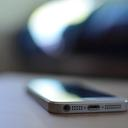
\includegraphics[width=7cm, height=7cm]{phone-unmodified.jpg}
	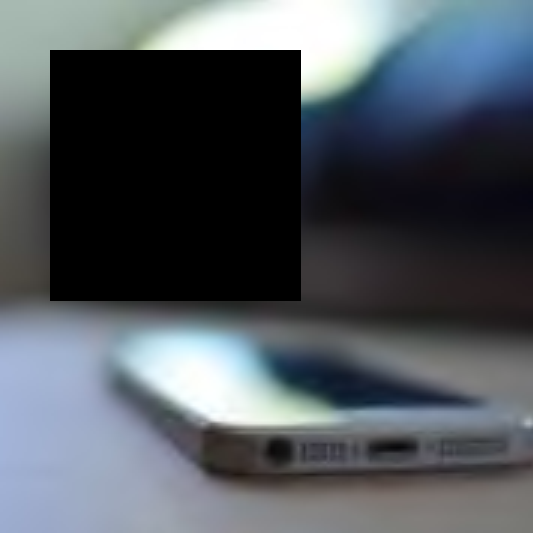
\includegraphics[width=7cm, height=7cm]{phone-crop.png}
\end{figure}
\subsection*{Kod źródłowy algorytmu}
\begin{python}
def crop(self, (x1, y1), (x2, y2)):
	print('croping image start')
	image = self.decoder.getPixels24Bits()
	
	print('croping')
	for x in range(x1, x2+1):
		for y in range(y1, y2+1):
			image[y, x] = (0, 0, 0)
	
	img = Image.fromarray(image, mode='RGB')
	img.save('Resources/Geometric-Crop.png')
	print('croping image done')
\end{python}
\section{Kopiowanie fragmentów obrazów}
\subsection*{Opis}
\begin{figure}[H]
	\caption{Przed uruchomieniem algorytmu (lewy), po skopiowaniu kwadratu od piksela \textit{(50, 50)} do \textit{(300, 300)} (prawy)}
	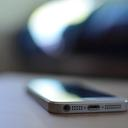
\includegraphics[width=7cm, height=7cm]{phone-unmodified.jpg}
	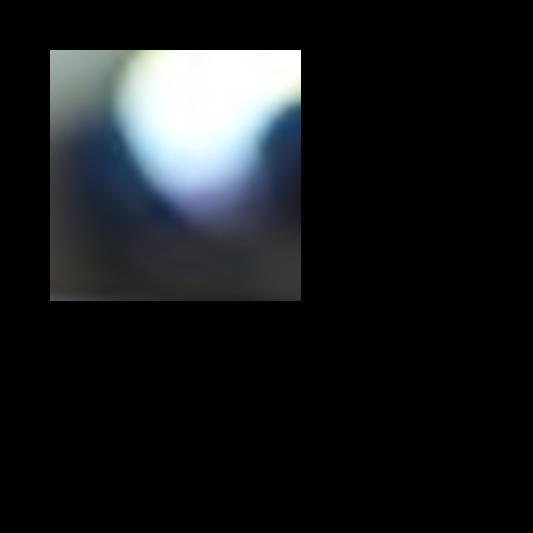
\includegraphics[width=7cm, height=7cm]{phone-copy.png}
\end{figure}
\subsection*{Kod źródłowy algorytmu}
\begin{python}
def copy(self, (x1, y1), (x2, y2)):
	print('copying image start')
	image = self.decoder.getPixels24Bits()
	height, width = self.decoder.height, self.decoder.width
	result = numpy.zeros((height, width, 3), numpy.uint8)
	
	print('copying')
	for x in range(x1, x2+1):
		for y in range(y1, y2+1):
			result[y, x] = image[y, x]
	
	img = Image.fromarray(result, mode='RGB')
	img.save('Resources/Geometric-Copy.png')
	print('copying image done')
\end{python}

\chapter{Operacje na histogramie obrazu szarego}
\section{Obliczanie histogramu}
\section{Przemieszczanie histogramu}
\section{Rozciąganie histogramu}
\section{Progowanie lokalne}
\section{Progowanie globalne}

\chapter{Operacje na histogramie obrazu barwowego}
\section{Obliczanie histogramu}
\section{Przemieszczanie histogramu}
\section{Rozciąganie histogramu}
\section{Progowanie 1-progowe lokalne}
\section{Progowanie wielo-progowe lokalne}
\section{Progowanie 1-progowe globalne}
\section{Progowanie wielo-progowe globalne}

\chapter{Operacje morfologiczne na obrazach binarnych}
Obrazy binarne mogą zawierać wiele niedoskonałości. W szczególności podczas tworzeniu obrazu binarnego z obrazu kolorowego \textit{(ang. tresholding)} zdarza się, że na obrazie wynikowym zostanie jakiś szum lub niechciany piksel. Operacje morfologiczne powstały aby umożliwić usuwanie tych niedoskonałości. 
\section{Erozja}
\subsection{Opis}
Okrawanie \textit{(ang. erosion)} oznacza \textbf{kurczenie} się zbioru czarnych połączonych pikseli co może prowadzić do kurczenia się elementów na obrazie jak i również usuwaniu połączeń pomiędzy elementami czy też wystających części elementu. W tym przykładzie do erozji używamy małego elementu strukturyzującego \textit{(ang. structuring element)} o wielkości 2x2. Użycie większego formatu skutkowałoby wycięciem większej połaci czarnych pikseli. 
\begin{figure}[H]
	\caption{Przed uruchomieniem algorytmu (lewy), po uruchomieniu erozji (prawy)}
	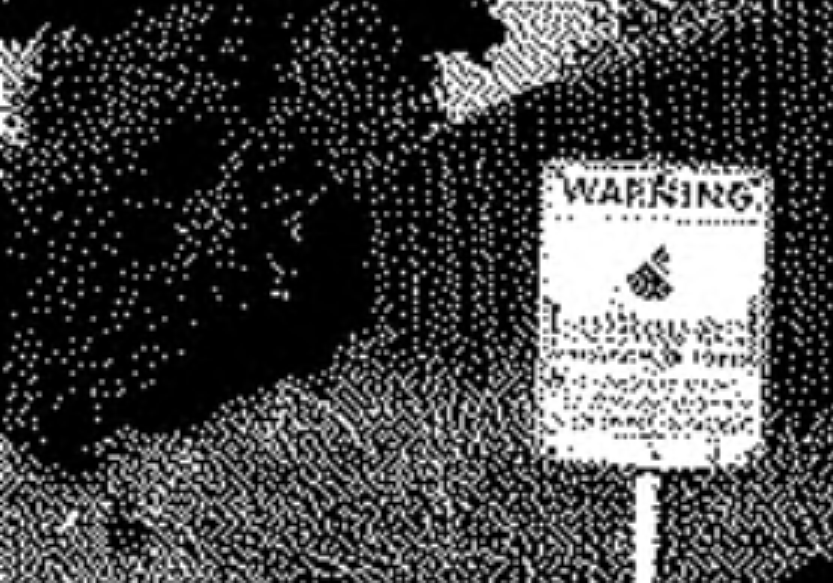
\includegraphics[width=7cm, height=7cm]{binary-unmodified.png}
	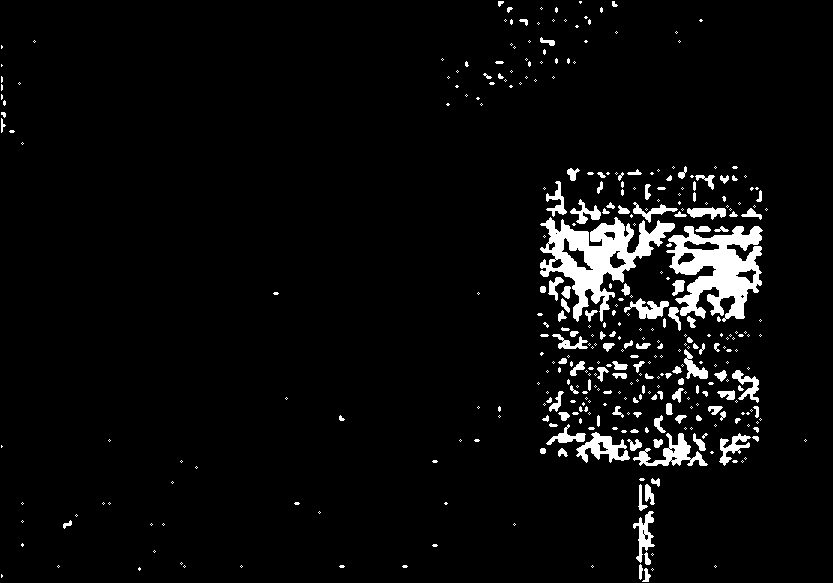
\includegraphics[width=7cm, height=7cm]{binary-erosion.png}
\end{figure}
\subsection{Kod źródłowy algorytmu}
\begin{python}
# Ex7.1
def erosion(self):
	print('erosion start')
	height, width = self.decoder.height, self.decoder.width
	image = self.decoder.getPixels()
	result = numpy.zeros((height, width), numpy.uint8)
	
	minY, minX = 1, 1
	maxY, maxX = height-1, width-1
	for y in range(minY, maxY):
		for x in range(minX, maxX):
			neighbourPixels = [255, 255, 255, 255]
	
			neighbourPixels[0]=(image[y][x-1])
			neighbourPixels[1]=(image[y-1][x])
			neighbourPixels[2]=(image[y][x+1])
			neighbourPixels[3]=(image[y+1][x])
	
			if 255 in neighbourPixels:
				result[y][x] = 255
			else:
				result[y][x] = 0
	
	img = Image.fromarray(result, mode='L')
	img.save('Resources/morph-erosion.png')
	print('erosion done')
\end{python}
\section{Dylatacja}
\subsection{Opis}
Nakładanie \textit{(ang. dilation)} oznacza \textbf{rozszerzanie} zbioru czarnych połączonych pikseli. Świetnie nadaje się do powiększaniu elementów obrazu jak i przy wypełnianiu luk w grupie białych pikseli. 
\begin{figure}[H]
	\caption{Przed uruchomieniem algorytmu (lewy), po dylatacji o element strukturyzujący 2x2 (prawy)}
	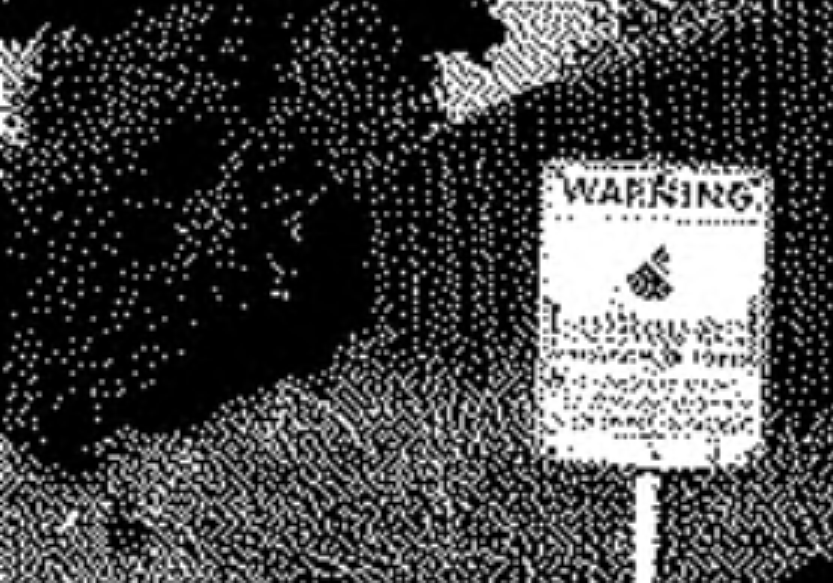
\includegraphics[width=7cm, height=7cm]{binary-unmodified.png}
	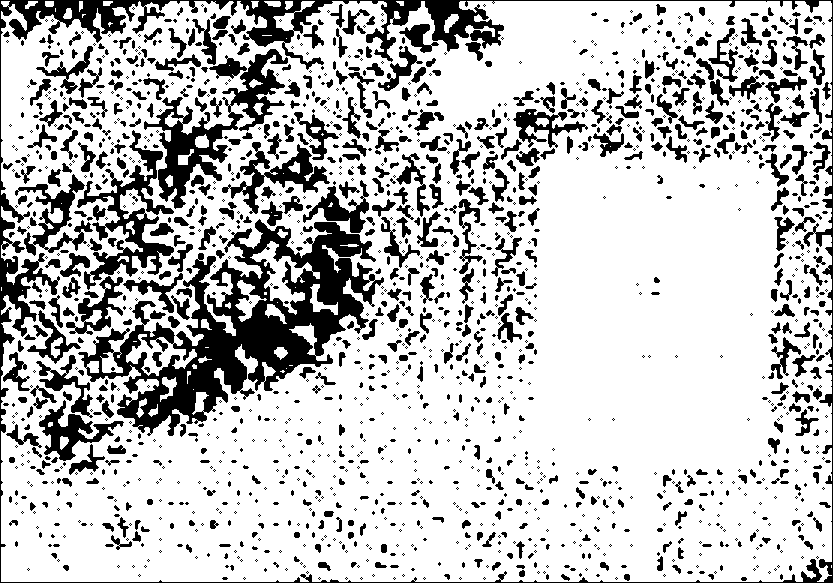
\includegraphics[width=7cm, height=7cm]{binary-dilation.png}
\end{figure}
\subsection{Kod źródłowy algorytmu}
\begin{python}
# Ex7.2
def dilation(self):
	print('dilation start')
	height, width = self.decoder.height, self.decoder.width
	image = self.decoder.getPixels()
	result = numpy.zeros((height, width), numpy.uint8)
	
	minY, minX = 1, 1
	maxY, maxX = height-1, width-1
	for y in range(minY, maxY):
		for x in range(minX, maxX):
			neighbourPixels = [255, 255, 255, 255]
	
			neighbourPixels[0]=(image[y][x-1])
			neighbourPixels[1]=(image[y-1][x])
			neighbourPixels[2]=(image[y][x+1])
			neighbourPixels[3]=(image[y+1][x])
			
			if 0 in neighbourPixels:
				result[y][x] = 0
			else:
				result[y][x] = 255
	
	img = Image.fromarray(result, mode='L')
	img.save('Resources/morph-dilation.png')
	print('dilation done')
\end{python}
\section{Otwarcie}
\subsection{Opis}
Wiele operacji morfologicznych składa się z kilku prostszych operacji takich jak: erozja, okrawanie lub nawet dopełnienie. Otwarcie jest jedną z takich operacji i jest złożeniem erozji poprzedzającej okrawanie. Nazwa tej operacji wzięła się od następstw jej użycia. Potrafi ona "otwierać" przerwy pomiędzy grupami pikseli, jeśli są one połączone cienkim "mostem". Zwiększenie elementu strukturalnego tej operacji spowoduje zwiększenie przerwy pomiędzy obiektami. 
\begin{figure}[H]
	\caption{Przed uruchomieniem algorytmu (lewy), po "otwarciu" (prawy)}
	\includegraphics[width=7cm, height=7cm]{binary-unmodified.png}
	\includegraphics[width=7cm, height=7cm]{binary-opening.png}
\end{figure}
\subsection{Kod źródłowy algorytmu}
\begin{python}
#Ex7.3
def opening(self):
	print('opening start')
	image = self.decoder.getPixels()
	
	result = self._erosionOperation(image)
	result = self._dilationOperation(result)
	
	img = Image.fromarray(result, mode='L')
	img.save('Resources/morph-opening.png')
	print('opening done')
	
def _dilationOperation(self, image):
	height, width = self.decoder.height, self.decoder.width
	result = numpy.zeros((height, width), numpy.uint8)
	
	minY, minX = 1, 1
	maxY, maxX = height-1, width-1
	for y in range(minY, maxY):
		for x in range(minX, maxX):
			neighbourPixels = [255, 255, 255, 255]
			
			neighbourPixels[0]=(image[y][x-1])
			neighbourPixels[1]=(image[y-1][x])
			neighbourPixels[2]=(image[y][x+1])
			neighbourPixels[3]=(image[y+1][x])
			
			if 0 in neighbourPixels:
				result[y][x] = 0
			else:
				result[y][x] = 255
	return result
	
def _erosionOperation(self, image):
	height, width = self.decoder.height, self.decoder.width
	result = numpy.zeros((height, width), numpy.uint8)
	
	minY, minX = 1, 1
	maxY, maxX = height-1, width-1
	for y in range(minY, maxY):
		for x in range(minX, maxX):
			neighbourPixels = [255, 255, 255, 255]
			
			neighbourPixels[0]=(image[y][x-1])
			neighbourPixels[1]=(image[y-1][x])
			neighbourPixels[2]=(image[y][x+1])
			neighbourPixels[3]=(image[y+1][x])
			
			if 255 in neighbourPixels:
				result[y][x] = 255
			else:
				result[y][x] = 0
	return result
\end{python}
\section{Zamknięcie}
\subsection{Opis}
Zamknięcie jest również złożeniem kilku operacji - tak jak otwarcie. Lecz w tym wypadku zamieniamy operacje wykorzystywane w otwarciu kolejnością. W ten sposób otrzymamy funkcję, która zamiast dzielić piksele łączy je bez zmiany ogólnego kształtu obiektu. Skuteczne przy "zamykaniu" dziur w obiektach. 
\begin{figure}[H]
	\caption{Przed uruchomieniem algorytmu (lewy), po zamknięciu (prawy)}
	\includegraphics[width=7cm, height=7cm]{binary-unmodified.png}
	\includegraphics[width=7cm, height=7cm]{binary-closing.png}
\end{figure}
\subsection{Kod źródłowy algorytmu}
\begin{python}
#Ex7.4
def closing(self):
	print('closing start')
	image = self.decoder.getPixels()
	
	result = self._dilationOperation(image)
	result = self._erosionOperation(result)
	
	img = Image.fromarray(result, mode='L')
	img.save('Resources/morph-closing.png')
	print('closing done')
	
def _dilationOperation(self, image):
	height, width = self.decoder.height, self.decoder.width
	result = numpy.zeros((height, width), numpy.uint8)
	
	minY, minX = 1, 1
	maxY, maxX = height-1, width-1
	for y in range(minY, maxY):
		for x in range(minX, maxX):
			neighbourPixels = [255, 255, 255, 255]
			
			neighbourPixels[0]=(image[y][x-1])
			neighbourPixels[1]=(image[y-1][x])
			neighbourPixels[2]=(image[y][x+1])
			neighbourPixels[3]=(image[y+1][x])
			
			if 0 in neighbourPixels:
				result[y][x] = 0
			else:
				result[y][x] = 255
	return result
	
def _erosionOperation(self, image):
	height, width = self.decoder.height, self.decoder.width
	result = numpy.zeros((height, width), numpy.uint8)
	
	minY, minX = 1, 1
	maxY, maxX = height-1, width-1
	for y in range(minY, maxY):
		for x in range(minX, maxX):
			neighbourPixels = [255, 255, 255, 255]
			
			neighbourPixels[0]=(image[y][x-1])
			neighbourPixels[1]=(image[y-1][x])
			neighbourPixels[2]=(image[y][x+1])
			neighbourPixels[3]=(image[y+1][x])
			
			if 255 in neighbourPixels:
				result[y][x] = 255
			else:
				result[y][x] = 0
	return result
\end{python}

\chapter{Operacje morfologiczne na obrazach szarych}
Operacje morfologiczne obrazów szarych to uogólnienie idei operacji morfologicznych na obrazach binarnych. Z zbioru wartości \textit{0, 255} przechodzimy do zbioru \textit{0, ..., 255}. Operacje OR i AND zastępujemy funkcjami Min i Max. Element strukturalny w tym rozdziale został rozbudowany o dwa elementy: o dynamiczną wielkość tablicy (z punktem centralnym w jej środku) pozwalającą na określenie zasięgu naszej operacji, oraz o wartości w elemencie pozwalające na określeniu głębi zmian koloru w obrazie. 
\section{Erozja}
\subsection{Opis}
Erozja w obrazach szarych sprowadza się do zwiększenia udziału ciemniejszych kolorów. Na zdjęciach po erozji można zaobserwować dwie zależności. Pierwsza z nich dotyczy wielkości elementu strukturalnego - im większy element tym większy efekt operacji, co można zobaczyć po pogrubieniu czarnych elementów. Natomiast nadanie elementowi wartości sprawi, że średnia wartość pikseli się obniży. 
\begin{figure}[H]
	\caption{Obraz niezmieniony (lewy), po erozji z użyciem elementu strukturalnego 3x3 o wartościach 50 (prawy)}
	\includegraphics[width=7cm, height=7cm]{man-unmodified.jpg}
	\includegraphics[width=7cm, height=7cm]{morph-gray-erosion-strel3x3-50.png}
\end{figure}
\begin{figure}[H]
	\caption{Obraz niezmieniony (lewy), po erozji z użyciem elementu strukturalnego 3x3 o wartościach 100 (prawy)}
	\includegraphics[width=7cm, height=7cm]{man-unmodified.jpg}
	\includegraphics[width=7cm, height=7cm]{morph-gray-erosion-strel3x3-100.png}
\end{figure}
\begin{figure}[H]
	\caption{Obraz niezmieniony (lewy), po erozji z użyciem elementu strukturalnego 10x10 o wartościach 0 (prawy)}
	\includegraphics[width=7cm, height=7cm]{man-unmodified.jpg}
	\includegraphics[width=7cm, height=7cm]{morph-gray-erosion-strel10x10-0.png}
\end{figure}
\begin{figure}[H]
	\caption{Obraz niezmieniony (lewy), po erozji z użyciem elementu strukturalnego 10x10 o wartościach 50 (prawy)}
	\includegraphics[width=7cm, height=7cm]{man-unmodified.jpg}
	\includegraphics[width=7cm, height=7cm]{morph-gray-erosion-strel10x10-50.png}
\end{figure}
\subsection{Kod źródłowy algorytmu}
\begin{python}
# Ex8.1
def erosion(self, seHeight, seWidth, seDepth):
	print('erosion start')
	image = self.decoder.getPixels()
	
	structuralElement = numpy.full((seHeight, seWidth), seDepth, numpy.uint8)
	result = self._erosionOperation(image, structuralElement, (4, 4))
	
	img = Image.fromarray(result, mode='L')
	img.save('Resources/morph-gray-erosion-strel{}x{}-{}.png'.format(str(seHeight), str(seWidth), str(seDepth)))
	print('erosion done')
def _erosionOperation(self, image, structuralElement, elementCenterIndices):
	image32 = image.copy().astype('int32')
	height, width = self.decoder.height, self.decoder.width
	result32 = numpy.zeros((height, width), numpy.int32)
	structuralElement32 = structuralElement.astype(numpy.int32)
	
	seHeight, seWidth = structuralElement32.shape
	seHalfY, seHalfX = seHeight-1-elementCenterIndices[0], seWidth-1-elementCenterIndices[1]
	minY, minX = seHalfY, seHalfX
	maxY, maxX = height-(seHeight-minY), width-(seWidth-minX)
	for y in range(minY, maxY):
		for x in range(minX, maxX):
			neighbourPixels = structuralElement32.copy()
			for seY in range(-seHalfY, seHalfY):
				for seX in range(-seHalfX, seHalfX):
					neighbourPixels[seY][seX] = image32[y+seY][x+seX] - structuralElement32[seY][seX]
			result32[y][x] = numpy.amin(neighbourPixels)
	result8 = numpy.clip(result32, 0, 255).astype('uint8')
	return result8
\end{python}
\section{Dylatacja}
\subsection{Opis}
	Okrawanie w wersji obrazów szarych sprowadza się do zmniejszenia udziału czerni. Po dylatacji można zaobserwować jak czarne obiekty ulegają zmniejszeniu i deformacji, oraz jak ogólna aparycja obrazu staje się jaśniejsza. Dzieje się tak z powodu funkcji \textit{max()}, która wybiera przy okrawaniu tylko najjaśniejsze sąsiedztwo piksela, oraz przez wartość elementu strukturalnego, która jest dodawana do wartości pikseli. Wadą większego elementu jest jego skłonność do zatracania szczegółów podczas dylatacji. 
\begin{figure}[H]
	\caption{Obraz niezmieniony (lewy), po dylatacji z użyciem elementu strukturalnego 5x5 o wartościach 50 (prawy)}
	\includegraphics[width=7cm, height=7cm]{man-unmodified.jpg}
	\includegraphics[width=7cm, height=7cm]{morph-gray-dilation-strel5x5-50.png}
\end{figure}
\begin{figure}[H]
	\caption{Obraz niezmieniony (lewy), po dylatacji z użyciem elementu strukturalnego 5x5 o wartościach 100 (prawy)}
	\includegraphics[width=7cm, height=7cm]{man-unmodified.jpg}
	\includegraphics[width=7cm, height=7cm]{morph-gray-dilation-strel5x5-100.png}
\end{figure}
\begin{figure}[H]
	\caption{Obraz niezmieniony (lewy), po dylatacji z użyciem elementu strukturalnego 10x10 o wartościach 0 (prawy)}
	\includegraphics[width=7cm, height=7cm]{man-unmodified.jpg}
	\includegraphics[width=7cm, height=7cm]{morph-gray-dilation-strel10x10-0.png}
\end{figure}
\begin{figure}[H]
	\caption{Obraz niezmieniony (lewy), po dylatacji z użyciem elementu strukturalnego 10x10 o wartościach 50 (prawy)}
	\includegraphics[width=7cm, height=7cm]{man-unmodified.jpg}
	\includegraphics[width=7cm, height=7cm]{morph-gray-dilation-strel10x10-50.png}
\end{figure}
\subsection{Kod źródłowy algorytmu}
\begin{python}
# Ex8.2
	def dilation(self, seHeight, seWidth, seDepth, seCenter=(0, 0)):
	print('dilation start')
	image = self.decoder.getPixels()
	
	structuralElement = numpy.full((seHeight, seWidth), seDepth, numpy.uint8)
	result = self._dilationOperation(image, structuralElement, seCenter)
	
	img = Image.fromarray(result, mode='L')
	img.save('Resources/morph-gray-dilation-strel{}x{}-{}.png'.format(str(seHeight), str(seWidth), str(seDepth)))
	print('dilation done')

def _dilationOperation(self, image, structuralElement, elementCenterIndices=(0, 0)):
	image32 = image.copy().astype('int32')
	height, width = self.decoder.height, self.decoder.width
	result32 = numpy.zeros((height, width), numpy.int32)
	structuralElement32 = structuralElement.astype(numpy.int32)
	
	seHeight, seWidth = structuralElement32.shape
	seHalfY, seHalfX = seHeight-1-elementCenterIndices[0], seWidth-1-elementCenterIndices[1]
	minY, minX = seHalfY, seHalfX
	maxY, maxX = height-(seHeight-minY), width-(seWidth-minX)
	for y in range(minY, maxY):
		for x in range(minX, maxX):
			neighbourPixels = structuralElement32.copy()
			for seY in range(-seHalfY, seHalfY):
				for seX in range(-seHalfX, seHalfX):
					neighbourPixels[seY][seX] = image32[y+seY][x+seX] + structuralElement32[seY][seX]
			result32[y][x] = numpy.amax(neighbourPixels)
	result8 = numpy.clip(result32, 0, 255).astype('uint8')
	return result8
\end{python}
\section{Otwarcie}
\subsection{Opis}
W obrazie binarnym otwarcie przyczyniało się do tworzenia przerw pomiędzy obiektami czarni. W wypadku obrazów szarych ta właściwość nie przepada, ale dochodzi jeszcze jedna wynikająca z wartości elementu strukturalnego. Im mniejsza jego wartość tym większy kontrast pomiędzy obiektami czerni i bieli. Na obrazach wynikowych widać również zatracenie szczegółów w oddali jak i również większą dominację jasno białego koloru. 
\begin{figure}[H]
	\caption{Obraz niezmieniony (lewy), po otwarciu z użyciem elementu strukturalnego 5x5 o wartościach 50 (prawy)}
	\includegraphics[width=7cm, height=7cm]{man-unmodified.jpg}
	\includegraphics[width=7cm, height=7cm]{morph-gray-opening-strel5x5-50.png}
\end{figure}
\begin{figure}[H]
	\caption{Obraz niezmieniony (lewy), po otwarciu z użyciem elementu strukturalnego 5x5 o wartościach 100 (prawy)}
	\includegraphics[width=7cm, height=7cm]{man-unmodified.jpg}
	\includegraphics[width=7cm, height=7cm]{morph-gray-opening-strel5x5-100.png}
\end{figure}
\begin{figure}[H]
	\caption{Obraz niezmieniony (lewy), po otwarciu z użyciem elementu strukturalnego 10x10 o wartościach 50 (prawy)}
	\includegraphics[width=7cm, height=7cm]{man-unmodified.jpg}
	\includegraphics[width=7cm, height=7cm]{morph-gray-opening-strel10x10-50.png}
\end{figure}
\begin{figure}[H]
	\caption{Obraz niezmieniony (lewy), po otwarciu z użyciem elementu strukturalnego 10x10 o wartościach 100 (prawy)}
	\includegraphics[width=7cm, height=7cm]{man-unmodified.jpg}
	\includegraphics[width=7cm, height=7cm]{morph-gray-opening-strel10x10-100.png}
\end{figure}
\subsection{Kod źródłowy algorytmu}
Funkcje erozji i okrawania są takie same jak w poprzednich sekcjach. 
\begin{python}
#Ex8.3
def opening(self, seHeight, seWidth, seDepth, seCenter=(0, 0)):
	print('opening start')
	image = self.decoder.getPixels()
	
	structuralElement = numpy.full((seHeight, seWidth), seDepth, numpy.uint8)
	result = self._erosionOperation(image, structuralElement, seCenter)
	result = self._dilationOperation(result, structuralElement, seCenter)
	
	img = Image.fromarray(result, mode='L')
	img.save('Resources/morph-gray-opening-strel{}x{}-{}.png'.format(str(seHeight), str(seWidth), str(seDepth)))
	print('opening done')
\end{python}
\section{Zamknięcie}
\begin{figure}[H]
	\caption{Obraz niezmieniony (lewy), po zamknięciu z użyciem elementu strukturalnego 5x5 o wartościach 50 (prawy)}
	\includegraphics[width=7cm, height=7cm]{man-unmodified.jpg}
	\includegraphics[width=7cm, height=7cm]{morph-gray-closing-strel5x5-50.png}
\end{figure}
\begin{figure}[H]
	\caption{Obraz niezmieniony (lewy), po zamknięciu z użyciem elementu strukturalnego 5x5 o wartościach 100 (prawy)}
	\includegraphics[width=7cm, height=7cm]{man-unmodified.jpg}
	\includegraphics[width=7cm, height=7cm]{morph-gray-closing-strel5x5-100.png}
\end{figure}
\begin{figure}[H]
	\caption{Obraz niezmieniony (lewy), po zamknięciu z użyciem elementu strukturalnego 10x10 o wartościach 50 (prawy)}
	\includegraphics[width=7cm, height=7cm]{man-unmodified.jpg}
	\includegraphics[width=7cm, height=7cm]{morph-gray-closing-strel10x10-50.png}
\end{figure}
\begin{figure}[H]
	\caption{Obraz niezmieniony (lewy), po zamknięciu z użyciem elementu strukturalnego 10x10 o wartościach 100 (prawy)}
	\includegraphics[width=7cm, height=7cm]{man-unmodified.jpg}
	\includegraphics[width=7cm, height=7cm]{morph-gray-closing-strel10x10-100.png}
\end{figure}
\subsection{Kod źródłowy algorytmu}
Funkcje erozji i okrawania są takie same jak w poprzednich sekcjach. 
\begin{python}
#Ex8.4
def closing(self, seHeight, seWidth, seDepth, seCenter=(0, 0)):
	print('closing start')
	image = self.decoder.getPixels()
	
	structuralElement = numpy.full((seHeight, seWidth), seDepth, numpy.uint8)
	result = self._dilationOperation(image, structuralElement, seCenter)
	result = self._erosionOperation(result, structuralElement, seCenter)
	
	img = Image.fromarray(result, mode='L')
	img.save('Resources/morph-gray-closing-strel{}x{}-{}.png'.format(str(seHeight), str(seWidth), str(seDepth)))
	print('closing done')
\end{python}

\chapter{Filtrowanie wygładzające liniowe i nieliniowe}
	Według definicji filtrowanie to technika modyfikująca lub upiększająca obraz. Dla przykładu, można nałożyć filtr na obraz w celu uwydatnienia jego krawędzi w taki sposób w jaki robi to filtr Robertsa. Przy czym filtr Robertsa należy do grupy filtrów liniowych co można poznać po operacjach jakie wykonuje. Głównie będą to proste operacje jak suma liniowa i będą się one wywodzić ze splotu różnych funkcji. W kategoriach filtrów znajdują się jeszcze filtry nieliniowe oparte na bazie kombinacji liniowych i heurystyk. Przykładem takiego filtru może być filtr medianowy. 
	\section{Filtr dolnoprzepustowy uśredniający}
		\subsection{Opis}
			Podstawowy filtr dający efekt rozmazania lub wygładzenia. Filtr oblicza średnią pikseli w elemencie strukturalnym (maska) o wielkości dziewięciu pikseli i przypisuje do piksela w środku. W swojej prostocie filtr ten ma słaby punkt w postaci szumu, który przejawia się w postaci białych, losowych pikseli. Po zastosowaniu filtru biały piksel może być bardziej widoczny niż wcześniej. \newline
			Maska tej operacji przedstawia się następująco:
			\begin{equation*}
				\quad
				\frac{1}{9}
				*
				\begin{bmatrix}
				1 & 1 & 1 \\
				1 & 1 & 1 \\
				1 & 1 & 1
				\end{bmatrix}
			\end{equation*}
			Dzięki niej jesteśmy w stanie symulować zachowanie oryginalnego filtru dolnoprzepustowego z elektroniki, który polegał na odcięciu górnych pasm częstotliwości w sygnale. Jednakże mając obraz w formacie macierzy trudno byłoby nam zgadnąć jaki piksel skrywa jaką wartość częstotliwości. Dlatego w tym temacie pomocny jest algorytm \textbf{Szybkiej Transformaty Fouriera} \textit{(ang. Fast Fourier Transform - FFT)}. Pozwala on na przeniesienie macierzy pikseli zawierającą wartości kolorów (domena czasu) w domenę częstotliwości. 
			\begin{figure}[H]
				\caption{Zmiana w częstotliwości obrazu przed i po zastosowaniu pokazanej maski}
				\includegraphics[width=15cm, height=15cm]{/overview/fft.png}
			\end{figure}
			\begin{figure}[H]
				\caption{Obraz niezmieniony (lewy), po zastosowaniu filtru z maską 9x9 (środkowy), z maską 27x27 (prawy)}
				\includegraphics[width=4cm, height=4cm]{man-unmodified.jpg}
				\includegraphics[width=4cm, height=4cm]{man-filter-boxblur9x9.png}
				\includegraphics[width=4cm, height=4cm]{man-filter-boxblur27x27.png}
			\end{figure}
		\subsection{Kod źródłowy algorytmu}
			\inputpython{../Source/Filters.py}{12}{37}
	\section{Filtr dolnoprzepustowy Gaussowski}
		\subsection{Opis}
			Kolejnym filtrem dolnoprzepustowym, wygładzającym obraz i usuwającym detale i szum jest filtr oparty o rozkład Gaussa. Ma ona zastosowanie przy produkcji maski dla tego filtra. Wartości maski, w swej idei, układają się w kształt dzwonu Gaussa (Rys. 10.3), tzn. największa wartość jest po środku macierzy, a wartości wokół niej tworzą pierścień składający się z mniejszych wartości. Jeśli wielkość maski na to pozwala kolejny pierścień mniejszych wartości otula poprzedni. \newline
			Przykładowe maski stworzone za pomocą funkcji Gaussa: 
			\begin{equation*}
				\frac{1}{16}
				*
				\begin{bmatrix}
				1 & 2 & 1 \\
				2 & 4 & 2 \\
				1 & 2 & 1
				\end{bmatrix}
				\quad
				\frac{1}{256}
				*
				\begin{bmatrix}
				1 & 4 & 6 & 4 & 1 \\
				4 & 16 & 24 & 16 & 4 \\
				6 & 24 & 36 & 24 & 6 \\
				4 & 16 & 24 & 16 & 4 \\
				1 & 4 & 6 & 4 & 1
				\end{bmatrix}
			\end{equation*}
			\begin{figure}[H]
				\caption{Dzwon Gaussa}
				\includegraphics[width=7cm, height=7cm]{overview/gauss-bell.png}
			\end{figure}
			Zaletą użycia rozkładu normalnego jest efekt jaki uzyskujemy w porównaniu do filtru uśredniającego. Rozkład normalny daje promieniście rozchodzącą się maskę, która z kolei nadaje wagi naszym pikselom. Używając wag do obliczania sumy w algorytmie filtra, uzyskujemy PSF \textit{(Point-spread function)} o okrągłym, kolistym kształcie. W porównaniu do poprzedniego rodzaju filtra, który zawsze daje nam rozmycie oparte o kształt prostokąta. 
			\begin{figure}[H]
				\caption{(Od lewej) Kropka bez rozmycia, rozmycie filtrem uśredniającym, rozmycie filtrem gaussowskim}
				\includegraphics[width=4cm, height=4cm]{overview/gauss-dot.jpg}
				\includegraphics[width=4cm, height=4cm]{overview/gauss-dot-boxblur.jpg}
				\includegraphics[width=4cm, height=4cm]{overview/gauss-dot-gaussianblur.jpg}
			\end{figure}
			\begin{figure}[H]
				\caption{Obraz niezmieniony (lewy), po zastosowaniu filtru z maską 9x9 i wartościami sumującymi się do 546 (środkowy), z maską 18x18 i wartościami sumującymi się do 1092 (prawy)}
				\includegraphics[width=4cm, height=4cm]{man-unmodified.jpg}
				\includegraphics[width=4cm, height=4cm]{man-filter-gaussianblur9x9f546.png}
				\includegraphics[width=4cm, height=4cm]{man-filter-gaussianblur18x18f1092.png}
			\end{figure}
		\subsection{Kod źródłowy algorytmu}
			\inputpython{../Source/Filters.py}{39}{70}
	\section{Filtr medianowy}
		\subsection{Opis}
			Filtr medianowy należy do rodziny filtrów nieliniowych, co oznacza że składa się on z kombinacji liniowych bądź opiera się na heurystyce. Po zastosowaniu go na zaszumiony obraz zdumiewamy się jego skutecznością w wale z białymi i/lub czarnymi pikselami. Natomiast po przyjrzeniu się możemy jeszcze dostrzec wyraźne linie krawędzi obiektów na obrazie co wyróżnia go na tle innych filtrów mogących usuwać szumy. Swoje niezwykłe, użyteczne właściwości filtr ten zawdzięcza kwartylowi rzędu 1/2, czyli medianie, która ignoruje wszystkie skrajne wartości w aktualnym oknie podczas wykonywania się algorytmu
			\begin{figure}[H]
				\caption{Obraz niezmieniony (lewy), po zastosowaniu filtru z maską 9x9 (środkowy), z maską 27x27 (prawy)}
				\includegraphics[width=4cm, height=4cm]{phone-noise-unmodified.jpg}
				\includegraphics[width=4cm, height=4cm]{phone-filter-median9x9.png}
				\includegraphics[width=4cm, height=4cm]{phone-filter-median27x27.png}
			\end{figure}
		\subsection{Kod źródłowy algorytmu}
			\inputpython{../Source/Filters.py}{72}{94}
	\section{Filtr modalny}
		\subsection{Opis}
			Filtr modalny bazuje na prostej statystyce. Podczas wykonywania algorytmu w oknie filtru jest obliczana ilość wystąpień wartości pikseli i na rezultat jest wybierana wartość występująca najczęściej. Jeśli wszystkie wartości występują tą samą ilość razy wtedy rezultatem jest aktualnie rozważany piksel. Filtr modalny produkuje gładkie, bezszumne obrazy. Czasem zdarza się, że obraz wyjściowy zawierał będzie obiekty z nieregularnymi kształtami, których nie było wcześniej. 
			\begin{figure}[H]
				\caption{Obraz niezmieniony (lewy, górny), po zastosowaniu filtru z maską 9x9 (prawy, górny), z maską 18x18 (lewy, dolny), z maską 27x27 (prawy, dolny)}
				\includegraphics[width=7cm, height=7cm]{man-noise-unmodified.jpg}
				\includegraphics[width=7cm, height=7cm]{man-filter-modal9x9.png}
				\includegraphics[width=7cm, height=7cm]{man-filter-modal18x18.png}
				\includegraphics[width=7cm, height=7cm]{man-filter-modal27x27.png}
			\end{figure}
			Dobranie odpowiedniej maski do obrazu jest kluczowe, aby filtr spełnił swoje zadanie. Siła tego algorytmu - statystyka - to równocześnie jego słabość. Mając obraz na którym króluje jeden lub kilka kolorów stajemy przed obliczem bezkształtnej jednokolorowej masy tego kolory po wykonaniu algorytmu jeśli źle dobierzemy wielkość maski. 
		\subsection{Kod źródłowy algorytmu}
			\inputpython{../Source/Filters.py}{96}{133}
	\section{Filtr Kuwahary}
		\subsection{Opis}
			Filtr wygładzający Kuwahary polega na w swojej idei na wybraniu jednego z czterech regionów, na które jest podzielona maska. Wybór odbywa się poprzez obliczenie odchylenia standardowego każdego regionu i wybranie tego który ma najmniejsze odchylenie. Każdy region nachodzi na krawędź dwóch sąsiednich. Im większa maska tym mniejsze jest rozmazanie krawędzi powstałe w wyniku usunięcia szumu. 
			\begin{figure}[H]
				\caption{Przykład maski z zaznaczonymi regionami}
				\includegraphics[width=16cm, height=7cm]{/overview/kuwahara-matrix.png}
			\end{figure}
			\begin{figure}[H]
				\caption{Obraz niezmieniony (lewy, górny), po zastosowaniu filtru z maską 3x3 (prawy, górny), z maską 9x9 (lewy, dolny), z maską 27x27 (prawy, dolny)}
				\includegraphics[width=7cm, height=7cm]{man-unmodified.jpg}
				\includegraphics[width=7cm, height=7cm]{man-filter-kuwahara3x3.png}
				\includegraphics[width=7cm, height=7cm]{man-filter-kuwahara9x9.png}
				\includegraphics[width=7cm, height=7cm]{man-filter-kuwahara27x27.png}
			\end{figure}
		\begin{figure}[H]
			\caption{Obraz niezmieniony (lewy, górny), po zastosowaniu filtru z maską 3x3 (prawy, górny), z maską 9x9 (lewy, dolny), z maską 27x27 (prawy, dolny)}
			\includegraphics[width=7cm, height=7cm]{phone-unmodified.jpg}
			\includegraphics[width=7cm, height=7cm]{phone-filter-kuwahara-color3x3.png}
			\includegraphics[width=7cm, height=7cm]{phone-filter-kuwahara-color9x9.png}
			\includegraphics[width=7cm, height=7cm]{phone-filter-kuwahara-color27x27.png}
		\end{figure}
		\subsection{Kod źródłowy algorytmu}
			\inputpython{../Source/Filters.py}{135}{199}
	\section{Filtr minimalny}
	\section{Filtr maksymalny}

\end{document}